\documentclass[11pt,openany]{book}

%% -------------------- Input and Microtypography --------------------
\usepackage[utf8]{inputenc}          % Unicode input
\usepackage{microtype}               % Improved typography

%% -------------------- Page Layout and Hyperlinks --------------------
\usepackage{geometry}
\geometry{a4paper, left=20mm, right=20mm, top=25mm, bottom=30mm}
\usepackage{hyperref}                % For clickable links
\usepackage{tocbibind}               % Include bibliography in TOC
\usepackage{titlesec}
%% -------------------- Math, Fonts, and Symbols --------------------
\usepackage{amsmath, amsfonts, amssymb, amsthm}
\usepackage{bm}

%% -------------------- Lists, Colors, and Graphics --------------------
\usepackage{enumitem}
\usepackage[table]{xcolor}
\usepackage{graphicx}
\usepackage{tikz}
\usetikzlibrary{circuits.logic.US,arrows.meta,positioning,calc,fit,decorations.markings,math}

%% -------------------- Tables, Code Listings, and Miscellaneous --------------------
\usepackage{booktabs}
\usepackage{listings}
\usepackage{adjustbox}
\usepackage{multirow}
\usepackage{fancyhdr}
\usepackage[normalem]{ulem}
\usepackage[document]{ragged2e}
\usepackage{venndiagram}
\usepackage{multicol}
\usepackage{algorithm}
\usepackage{algpseudocode}
\usepackage{wrapfig}
\usepackage{circuitikz}
\usepackage{caption}
\usepackage{media9}

%% -------------------- Page Headers and Footers --------------------
\pagestyle{fancy}
\fancyhf{} % clear all header/footer fields
\fancyhead[RE]{\leftmark}             % Left header on even pages: chapter info
\fancyhead[RO]{Notes by Ali EL AZDI}   % Right header on odd pages: custom text
\fancyfoot[CE,CO]{\thepage}            % Center page number on all pages
\renewcommand{\headrulewidth}{0pt}
\renewcommand{\footrulewidth}{0pt}

%% -------------------- Custom Commands --------------------
\newcommand*\xor{\oplus}
\newcommand{\minidash}{\text{-}}

% A custom vertical spacing command
\usepackage{etoolbox}
\makeatletter
\newcommand{\vspacer}[1]{%
  \ifvmode
    \vskip#1\relax
  \else
    \@bsphack
    \vadjust{\vskip#1\relax}
    \@esphack
  \fi
}
\makeatother
%%%%%%%%%%%%%%%%%%% Verilog CODE STYLING %%%%%%%%%%%%%%%%%%%%%%%%%%%%%
\definecolor{keywordcolor}{rgb}{0.5,0.0,0.33}
\definecolor{backgroundcolor}{rgb}{0.95,0.95,1.0}
\definecolor{commentcolor}{rgb}{0.129,0.384,0.529}
\definecolor{stringcolor}{rgb}{0.16,0.00,1.00}
\definecolor{rulecolor}{rgb}{0.46,0.43,0.5}
\definecolor{codegray}{rgb}{0.5,0.5,0.5}

\lstdefinestyle{verilogstyle}{
  language=Verilog,
  basicstyle=\ttfamily\footnotesize,
  backgroundcolor=\color{backgroundcolor},
  commentstyle=\color{commentcolor}\ttfamily, % Add \ttfamily to ensure comments are in typewriter font
  morecomment=[l][\color{commentcolor}\ttfamily]{//}, % Line comment in Verilog
  morecomment=[s][\color{commentcolor}\ttfamily]{/*}{*/}, % Block comments in Verilog
  morekeywords={module, input, output, wire, endmodule, endcase, default, tri, assign, always, if, else, begin, end, case, endcase, parameter}, % Add Verilog keywords
  keywordstyle=\color{keywordcolor},
  stringstyle=\color{stringcolor},
  showstringspaces=false,
  frame=single,
  rulecolor=\color{rulecolor}, % Frame color
  breaklines=true,
  numbers=left,
  numberstyle=\tiny\color{codegray},
  tabsize=2
}

\lstnewenvironment{verilog}
  {\lstset{style=verilogstyle}}
  {}


%%%%%%%%%%%%%%%%%%% C CODE STYLING %%%%%%%%%%%%%%%%%%%%%%%%%%%%%
\usepackage{xcolor}
\usepackage{listings}

% Define custom colors for C syntax highlighting
\definecolor{CKeyWord}{rgb}{0.8,0.1,0.1}      % For C keywords (e.g., int, return)
\definecolor{CBackground}{rgb}{0.95,0.95,0.95} % Background color for code blocks
\definecolor{CComment}{rgb}{0.0,0.5,0.0}        % Comment color
\definecolor{CString}{rgb}{0.1,0.1,0.8}         % String literal color
\definecolor{CRule}{rgb}{0.5,0.5,0.5}           % Frame rule color
\definecolor{CNumber}{rgb}{0.6,0.6,0.6}         % Line number color

% Define a custom listing style for C code
\lstdefinestyle{CStyle}{
  language=C,
  basicstyle=\footnotesize\ttfamily,
  backgroundcolor=\color{CBackground},
  commentstyle=\color{CComment}\itshape,
  keywordstyle=\color{CKeyWord}\bfseries,
  stringstyle=\color{CString},
  numbers=left,
  numberstyle=\tiny\color{CNumber},
  stepnumber=1,
  numbersep=10pt,
  showspaces=false,
  showstringspaces=false,
  breaklines=true,
  frame=single,
  rulecolor=\color{CRule},
  tabsize=2,
  captionpos=b,
  columns=fullflexible,
  keepspaces=true,
}

% Define a new environment for C code blocks using the custom style.
% Optional arguments can be passed to adjust settings further.
\lstnewenvironment{cc}[1][]{
  \lstset{style=CStyle, #1}
}{}
%%%%%%%%%%%%%%%%%%% Assembly CODE STYLING %%%%%%%%%%%%%%%%%%%%%%%%%%%%%
\definecolor{akeywordcolor}{rgb}{0.0, 0.2, 0.4}
\definecolor{abackgroundcolor}{rgb}{0.98, 0.99, 1.0}
\definecolor{acommentcolor}{rgb}{0.0, 0.4, 0.6}
\definecolor{astringcolor}{rgb}{0.2, 0.4, 0.8}
\definecolor{arulecolor}{rgb}{0.6, 0.7, 0.8}
\definecolor{acodegray}{rgb}{0.3, 0.4, 0.5}

\lstdefinestyle{assembly}{
  language=[x86masm]Assembler,
  basicstyle=\ttfamily\footnotesize,
  backgroundcolor=\color{abackgroundcolor},
  commentstyle=\color{acommentcolor}\ttfamily,
  keywordstyle=\color{akeywordcolor},
  stringstyle=\color{astringcolor},
  showstringspaces=false,
  frame=single,
  rulecolor=\color{arulecolor},
  breaklines=true,
  numbers=left,
  numberstyle=\tiny\color{acodegray},
  tabsize=2,
  morekeywords={li, and, add, addi, srli, bne}
}

\lstnewenvironment{assembly}
  {\lstset{style=assembly}}
  {}

%%%%%%%%%%%%%%%%%%% JAVA CODE STYLING %%%%%%%%%%%%%%%%%%%%%%%%%%%%%
\definecolor{javakeywordcolor}{rgb}{0.0, 0.0, 0.5}
\definecolor{javabackgroundcolor}{rgb}{0.95, 0.95, 0.95}
\definecolor{javacommentcolor}{rgb}{0.0, 0.5, 0.0}
\definecolor{javastringcolor}{rgb}{0.6, 0.0, 0.0}
\definecolor{javarulecolor}{rgb}{0.5, 0.5, 0.5}
\definecolor{javagray}{rgb}{0.6, 0.6, 0.6}

\lstdefinestyle{javastyle}{
  language=Java,
  basicstyle=\ttfamily\footnotesize,
  backgroundcolor=\color{javabackgroundcolor},
  commentstyle=\color{javacommentcolor}\ttfamily,
  keywordstyle=\color{javakeywordcolor},
  stringstyle=\color{javastringcolor},
  showstringspaces=false,
  frame=single,
  rulecolor=\color{javarulecolor},
  breaklines=true,
  numbers=left,
  numberstyle=\tiny\color{javagray},
  tabsize=2,
  morekeywords={class, public, private, protected, extends, implements, interface, import, package, new, return, void, static}
}

\lstnewenvironment{java}
  {\lstset{style=javastyle}}
  {}




%% -------------------- Custom Definition Environment --------------------
\makeatletter
\newenvironment{definition}[1][]{%
  % Add an entry to the TOC: if a title is provided, include it.
  \ifstrempty{#1}%
    {\addcontentsline{toc}{subsection}{Definition}}%
    {\addcontentsline{toc}{subsection}{Definition: #1}}%
  % Print the heading: include the title if given.
  \par\noindent\textbf{Definition\ifstrempty{#1}{}{ (#1)}.}\quad\itshape%
}{\par}
\makeatother
% Other theorem-like environments
\newtheorem{example}{Example}[subsection]
\newtheorem{theorem}{Theorem}[subsection]
\titlespacing{\section}{0pt}{10pt}{5pt} % {left}{before}{after}
%% -------------------- Document Begins --------------------
\begin{document}
\raggedbottom

% Title Page
\begin{titlepage}
    \centering
    \vspace*{1cm}
    \Huge
    Computer Systems \newline
    \vspace{10px}
    \LARGE IN BA4
    \vspace*{10px}
    \newline
    \Large Notes by Ali EL AZDI

    \vfill
    \large
    September 11, 2024
\end{titlepage}

\begin{center}
    \vspace*{1cm}
    \textbf{Introduction}
    \newline
    \paragraph[short]{}{This document is designed to offer a LaTeX-styled overview of the Computer Systems course, emphasizing brevity and clarity. Should there be any inaccuracies or areas for improvement, please reach out at ali.elazdi@epfl.ch for corrections. For the latest version of the PDF, you can check the following link: 
    \url{https://elazdi-al.github.io/compsys/index.html}. Feel free to send a pull request to propose any changes you think might be a useful addition to the course content or a modification.}
    \newline
   \url{
        https://github.com/elazdi-al/compsys/blob/main/main.pdf
    }
    \newline
\end{center}


% Table of Contents
\tableofcontents

 

\chapter{Lecture 01: Introduction}

In this lecture we explore the journey of a YouTube video—from its storage as a file to its transformation into bytes, its transmission over networks, and finally, its display on your device. We will introduce key concepts such as processes, threads, distributed applications, system calls, and the role of the operating system in managing hardware resources.
\vfill
%%%%%%%%%%%%%%%%%%%%%%%%%%%%%%%%%%%%%%%%%%%%%%%%%%%%%%%%%%%%%%%%%%%%%%
\section{The Journey of a YouTube Video}
To illustrate these ideas, consider the journey of a YouTube video. The video begins its existence as a file stored on a storage device, is loaded into memory as bytes, transmitted as packets over the Internet, and finally rendered on your screen.

\begin{center}
  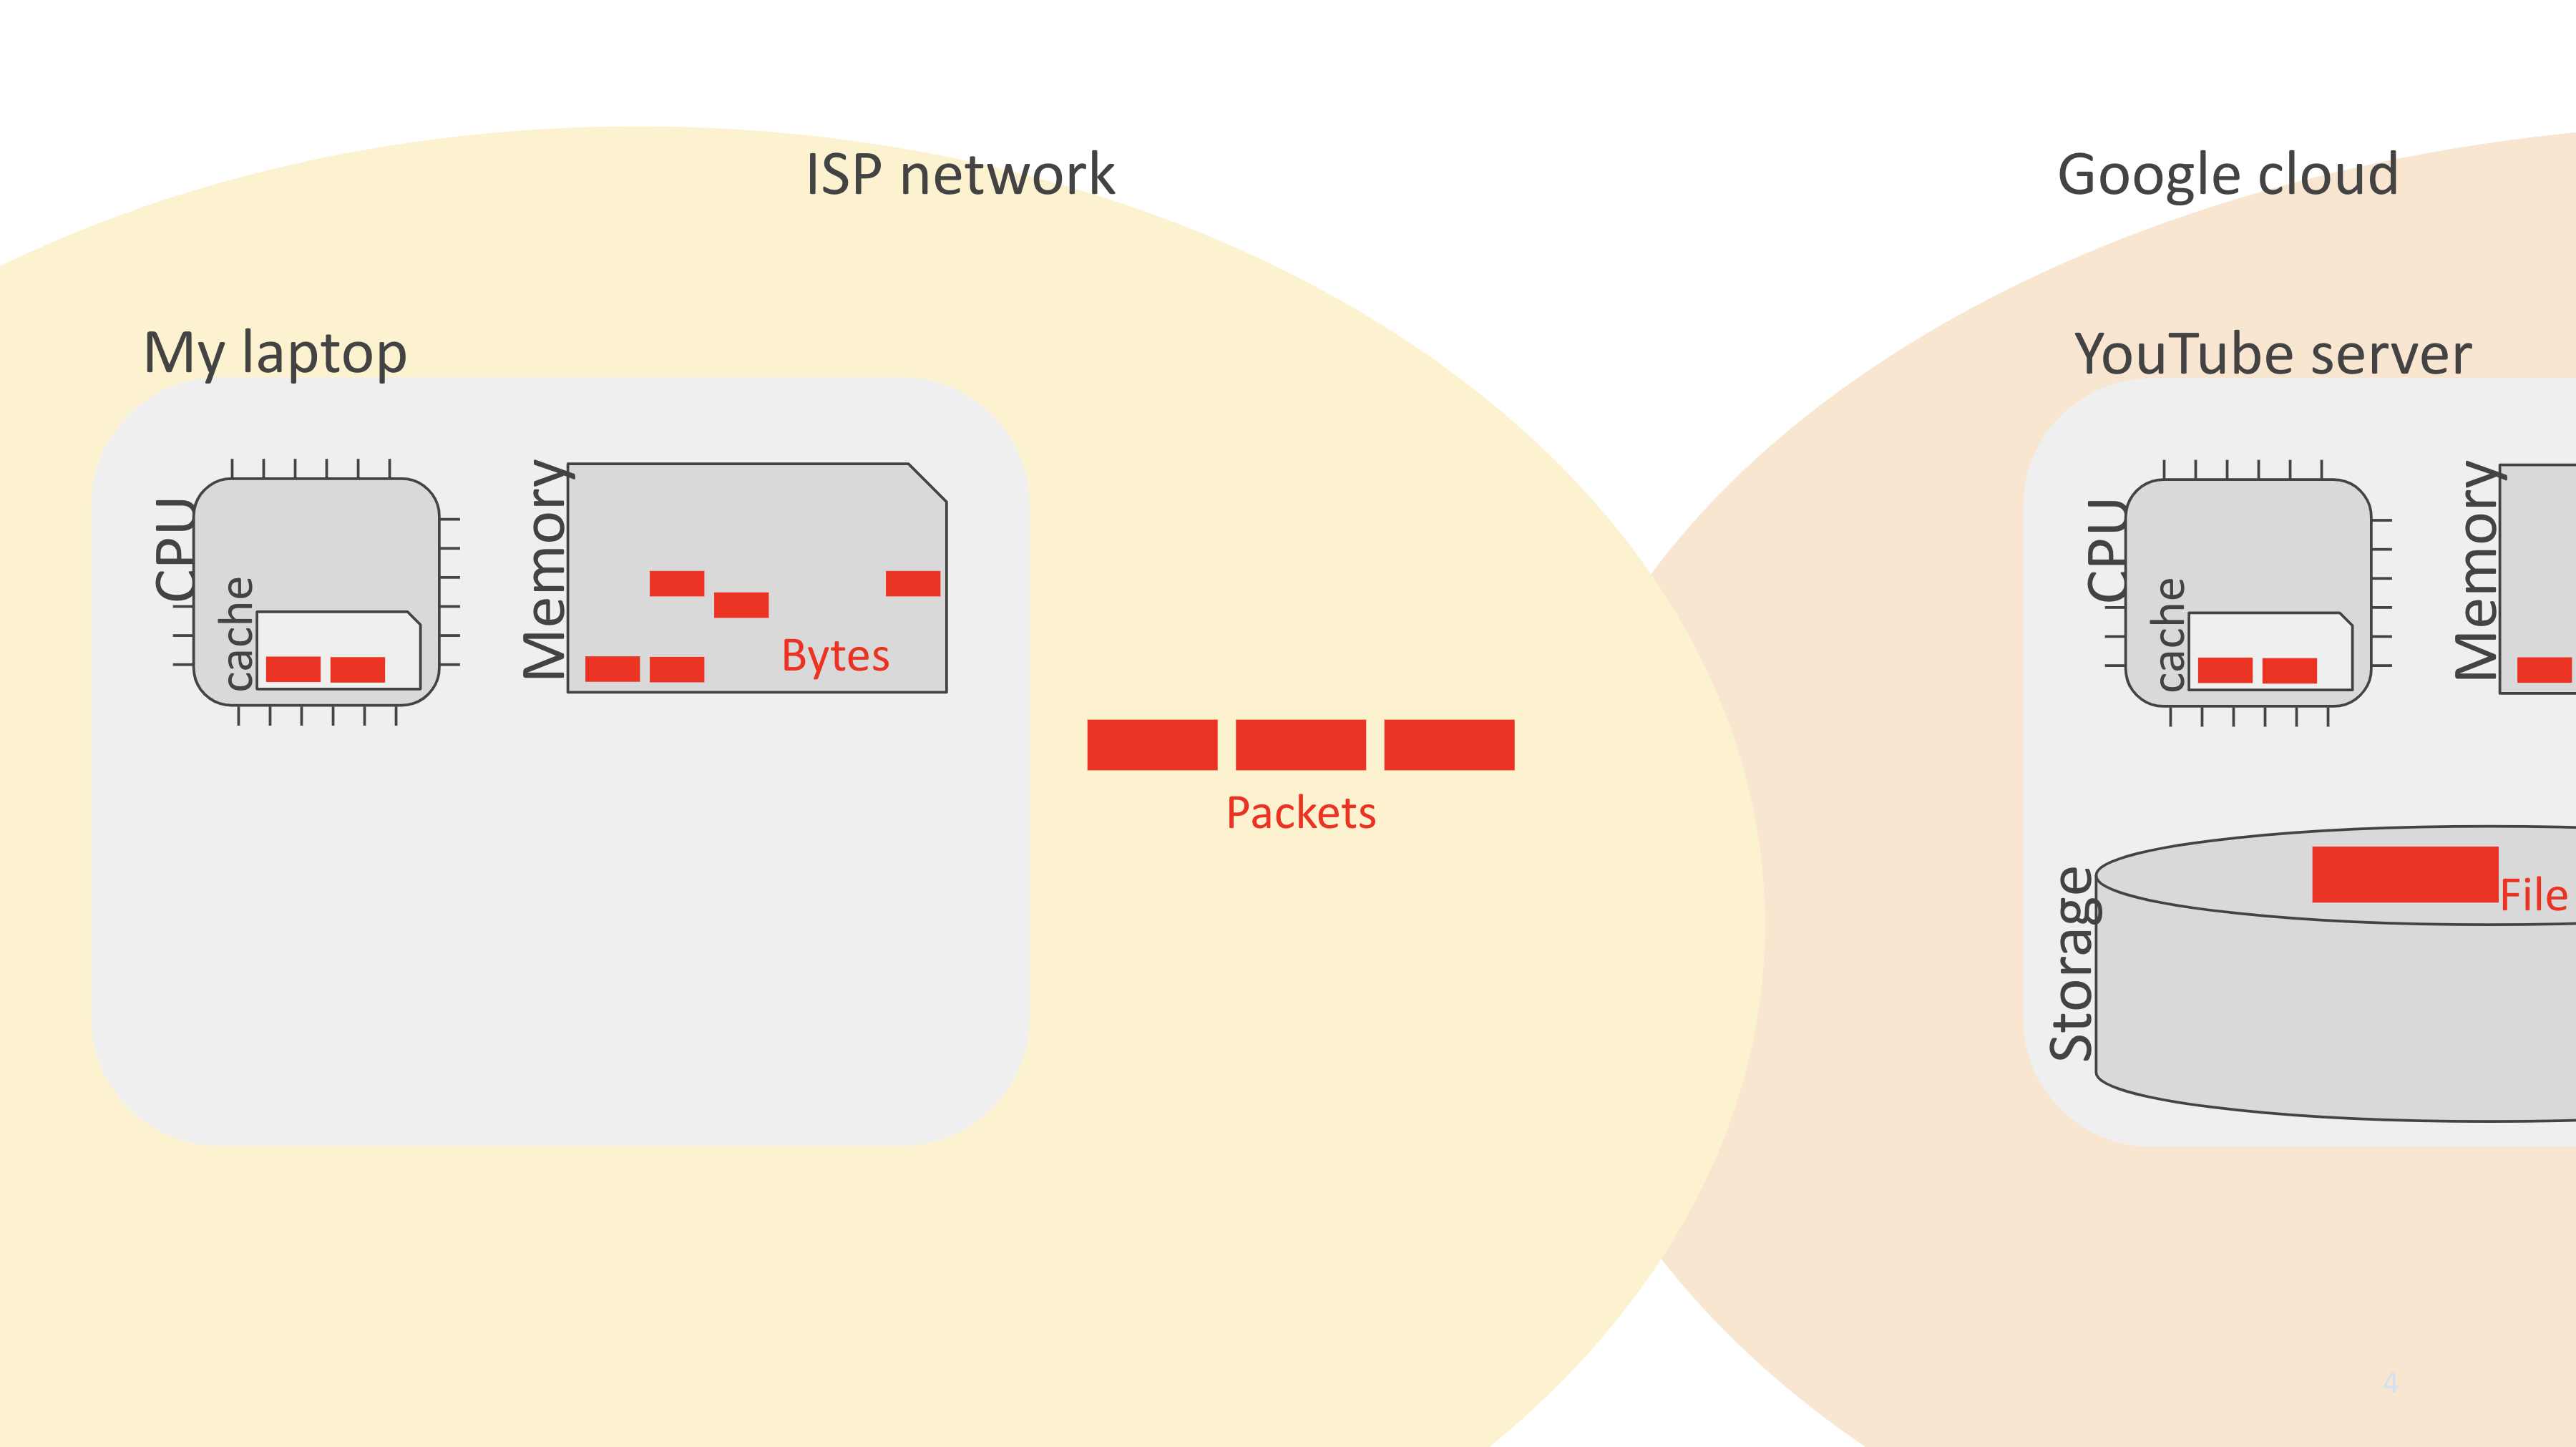
\includegraphics[width=0.85\textwidth]{chapters/L1/images/youtube.png}
\end{center}
\newpage
%%%%%%%%%%%%%%%%%%%%%%%%%%%%%%%%%%%%%%%%%%%%%%%%%%%%%%%%%%%%%%%%%%%%%%
\subsection{Start of the Journey: Inside the Laptop}
The journey begins on your laptop.\\[5px] 
\begin{minipage}{0.45\textwidth}
  \begin{justify}
    A computer hosts many different programs (e.g., a web browser, a ping utility, a git client). These programs, stored as files on disk, are invoked by user actions such as clicking an icon or typing a command. When a program is invoked, the computer creates a new \emph{process} in main memory. A process represents a running instance of a program and may consist of one or more \emph{threads}—individual units of execution within the process.
  \end{justify}
\end{minipage}
\hfill
\vline
\hfill
\begin{minipage}{0.45\textwidth}
  \begin{center}
  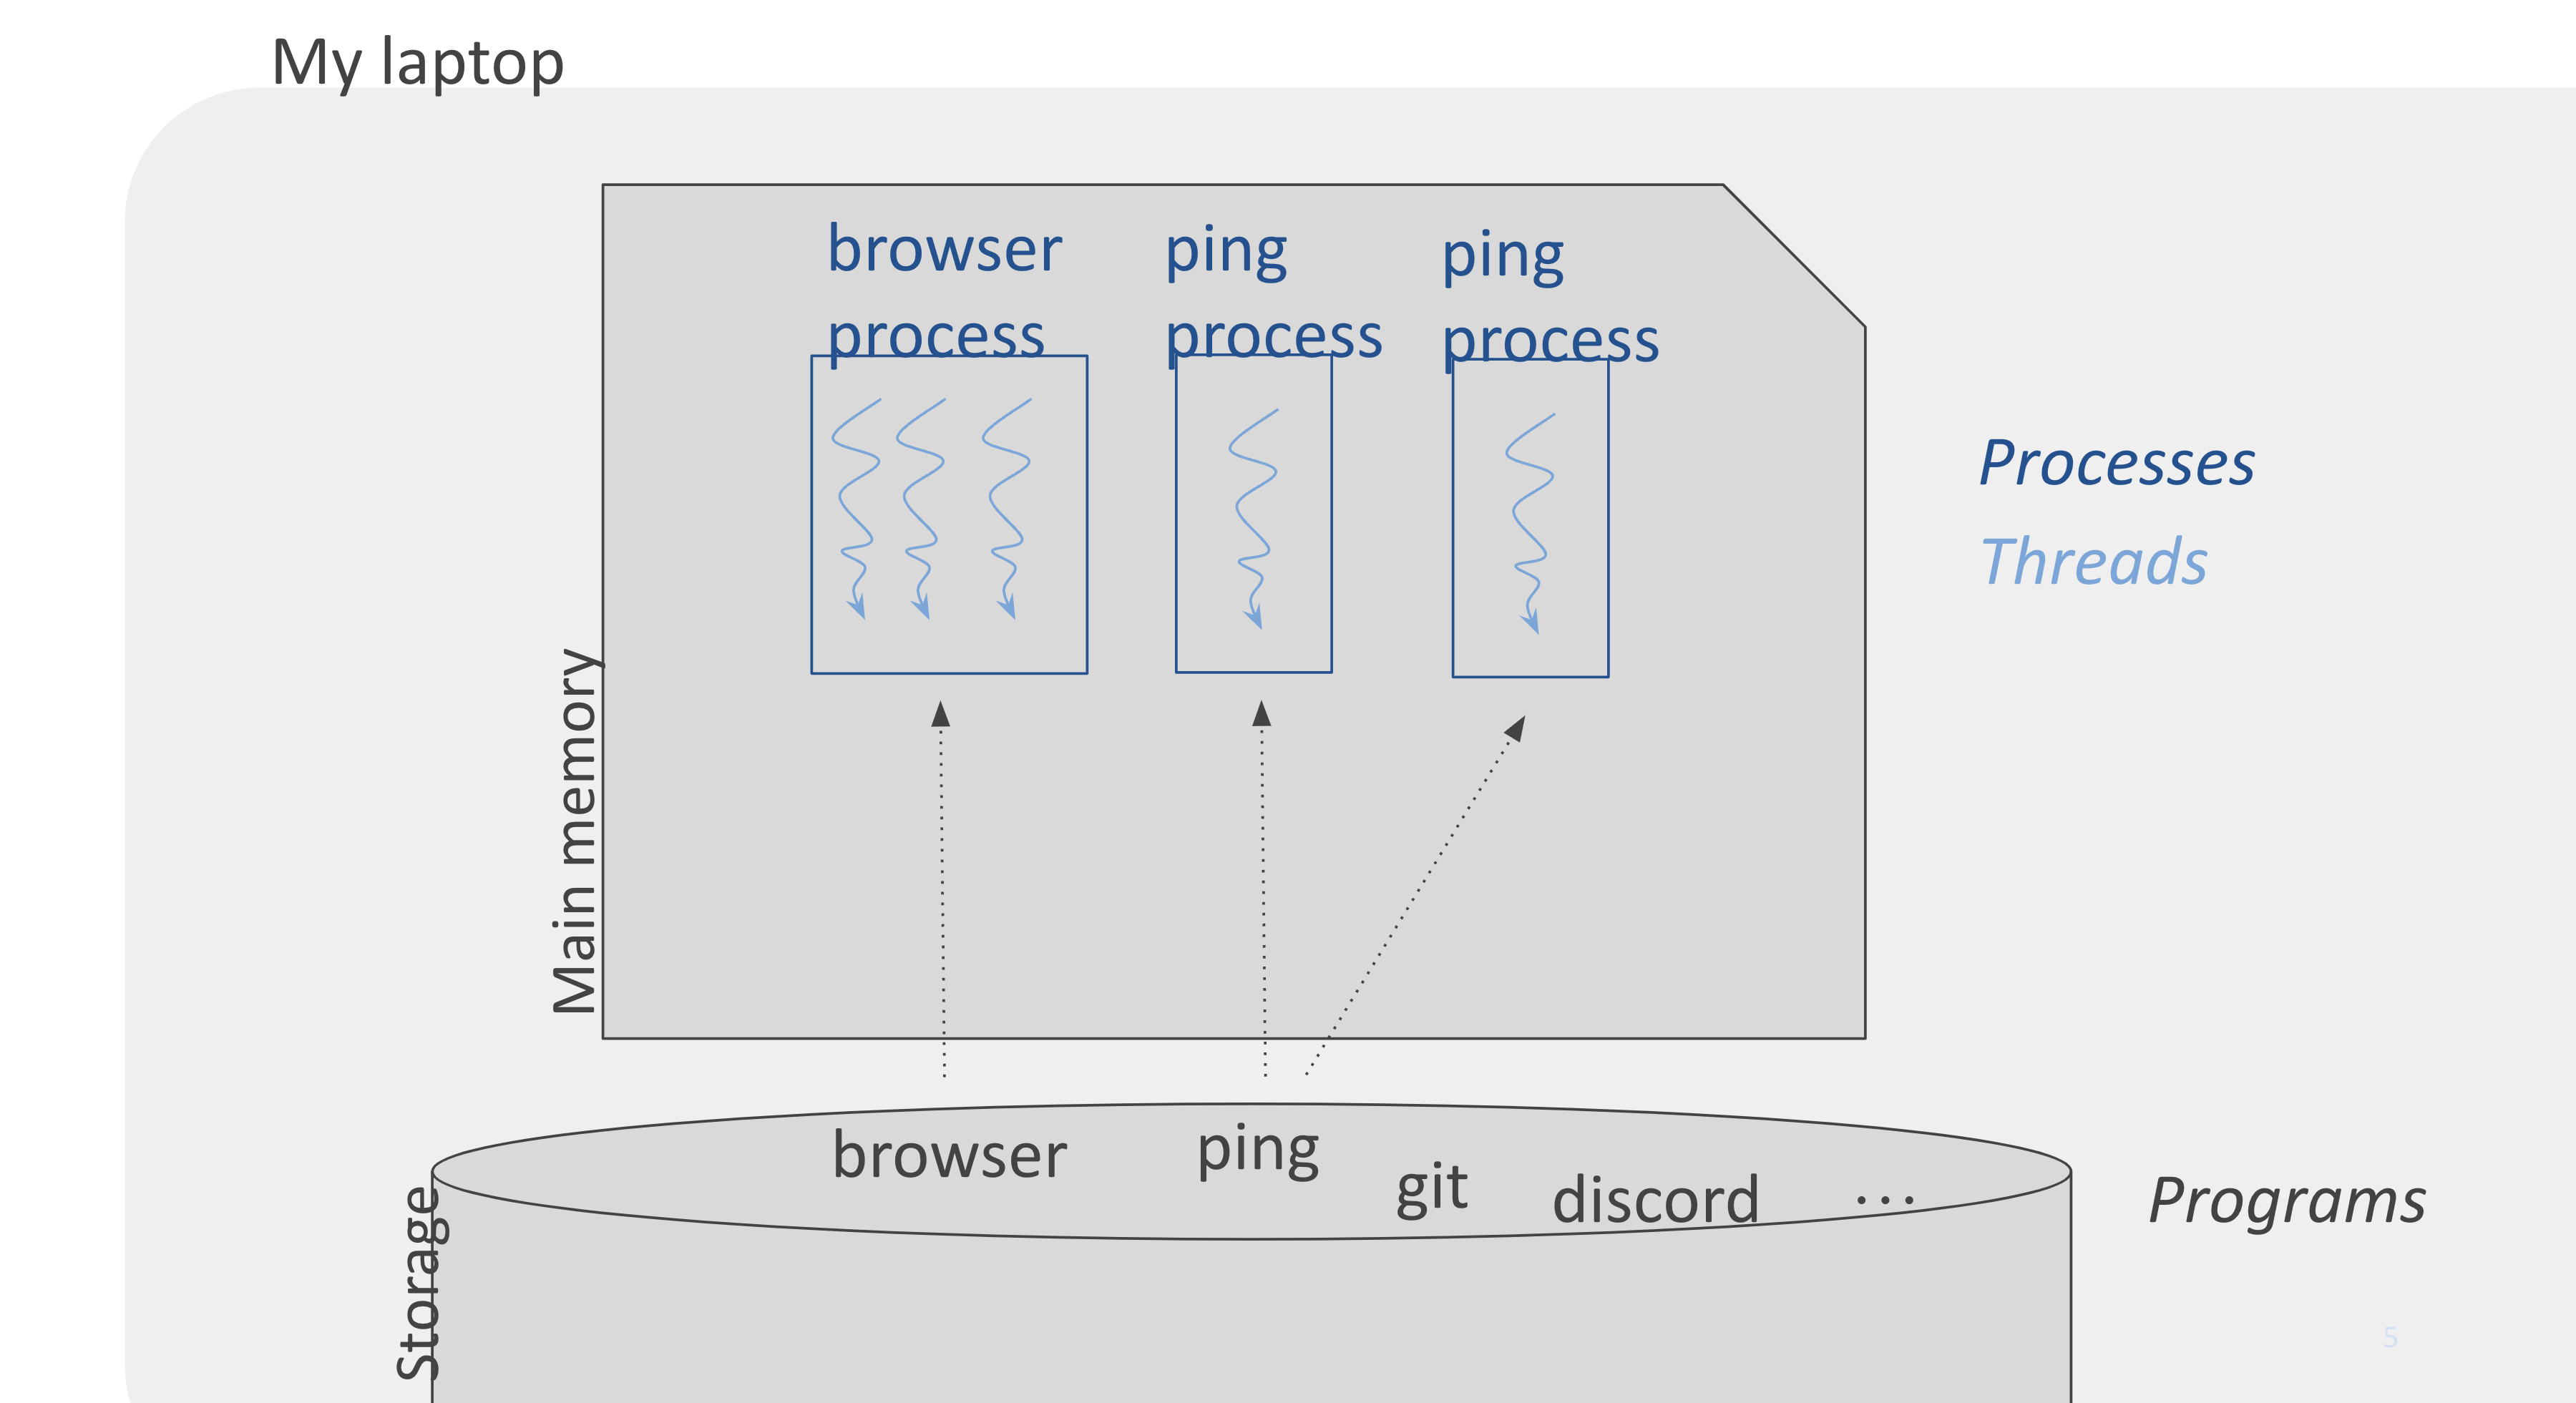
\includegraphics[width=1.2\textwidth]{chapters/L1/images/threads.png}
\end{center}
\end{minipage}\vfill
\vfill
\begin{definition}[Program, Process, Thread]
A \textbf{program} is a set of instructions stored as a file on disk. When a program is invoked, the computer creates a \textbf{process}—a running instance of that program in main memory. A process may consist of one or more \textbf{threads}, which are the individual sequences of execution within the process.
\end{definition}

%%%%%%%%%%%%%%%%%%%%%%%%%%%%%%%%%%%%%%%%%%%%%%%%%%%%%%%%%%%%%%%%%%%%%jjjj%
\vfill
\subsection{Accessing a Video: A Distributed Application}

When you use your web browser to access a video, the browser sends a message (or request) to a remote YouTube server. The browser process (running on your laptop) and the server process (running on a different computer) work together as parts of a \emph{distributed application}. 
\begin{center}
  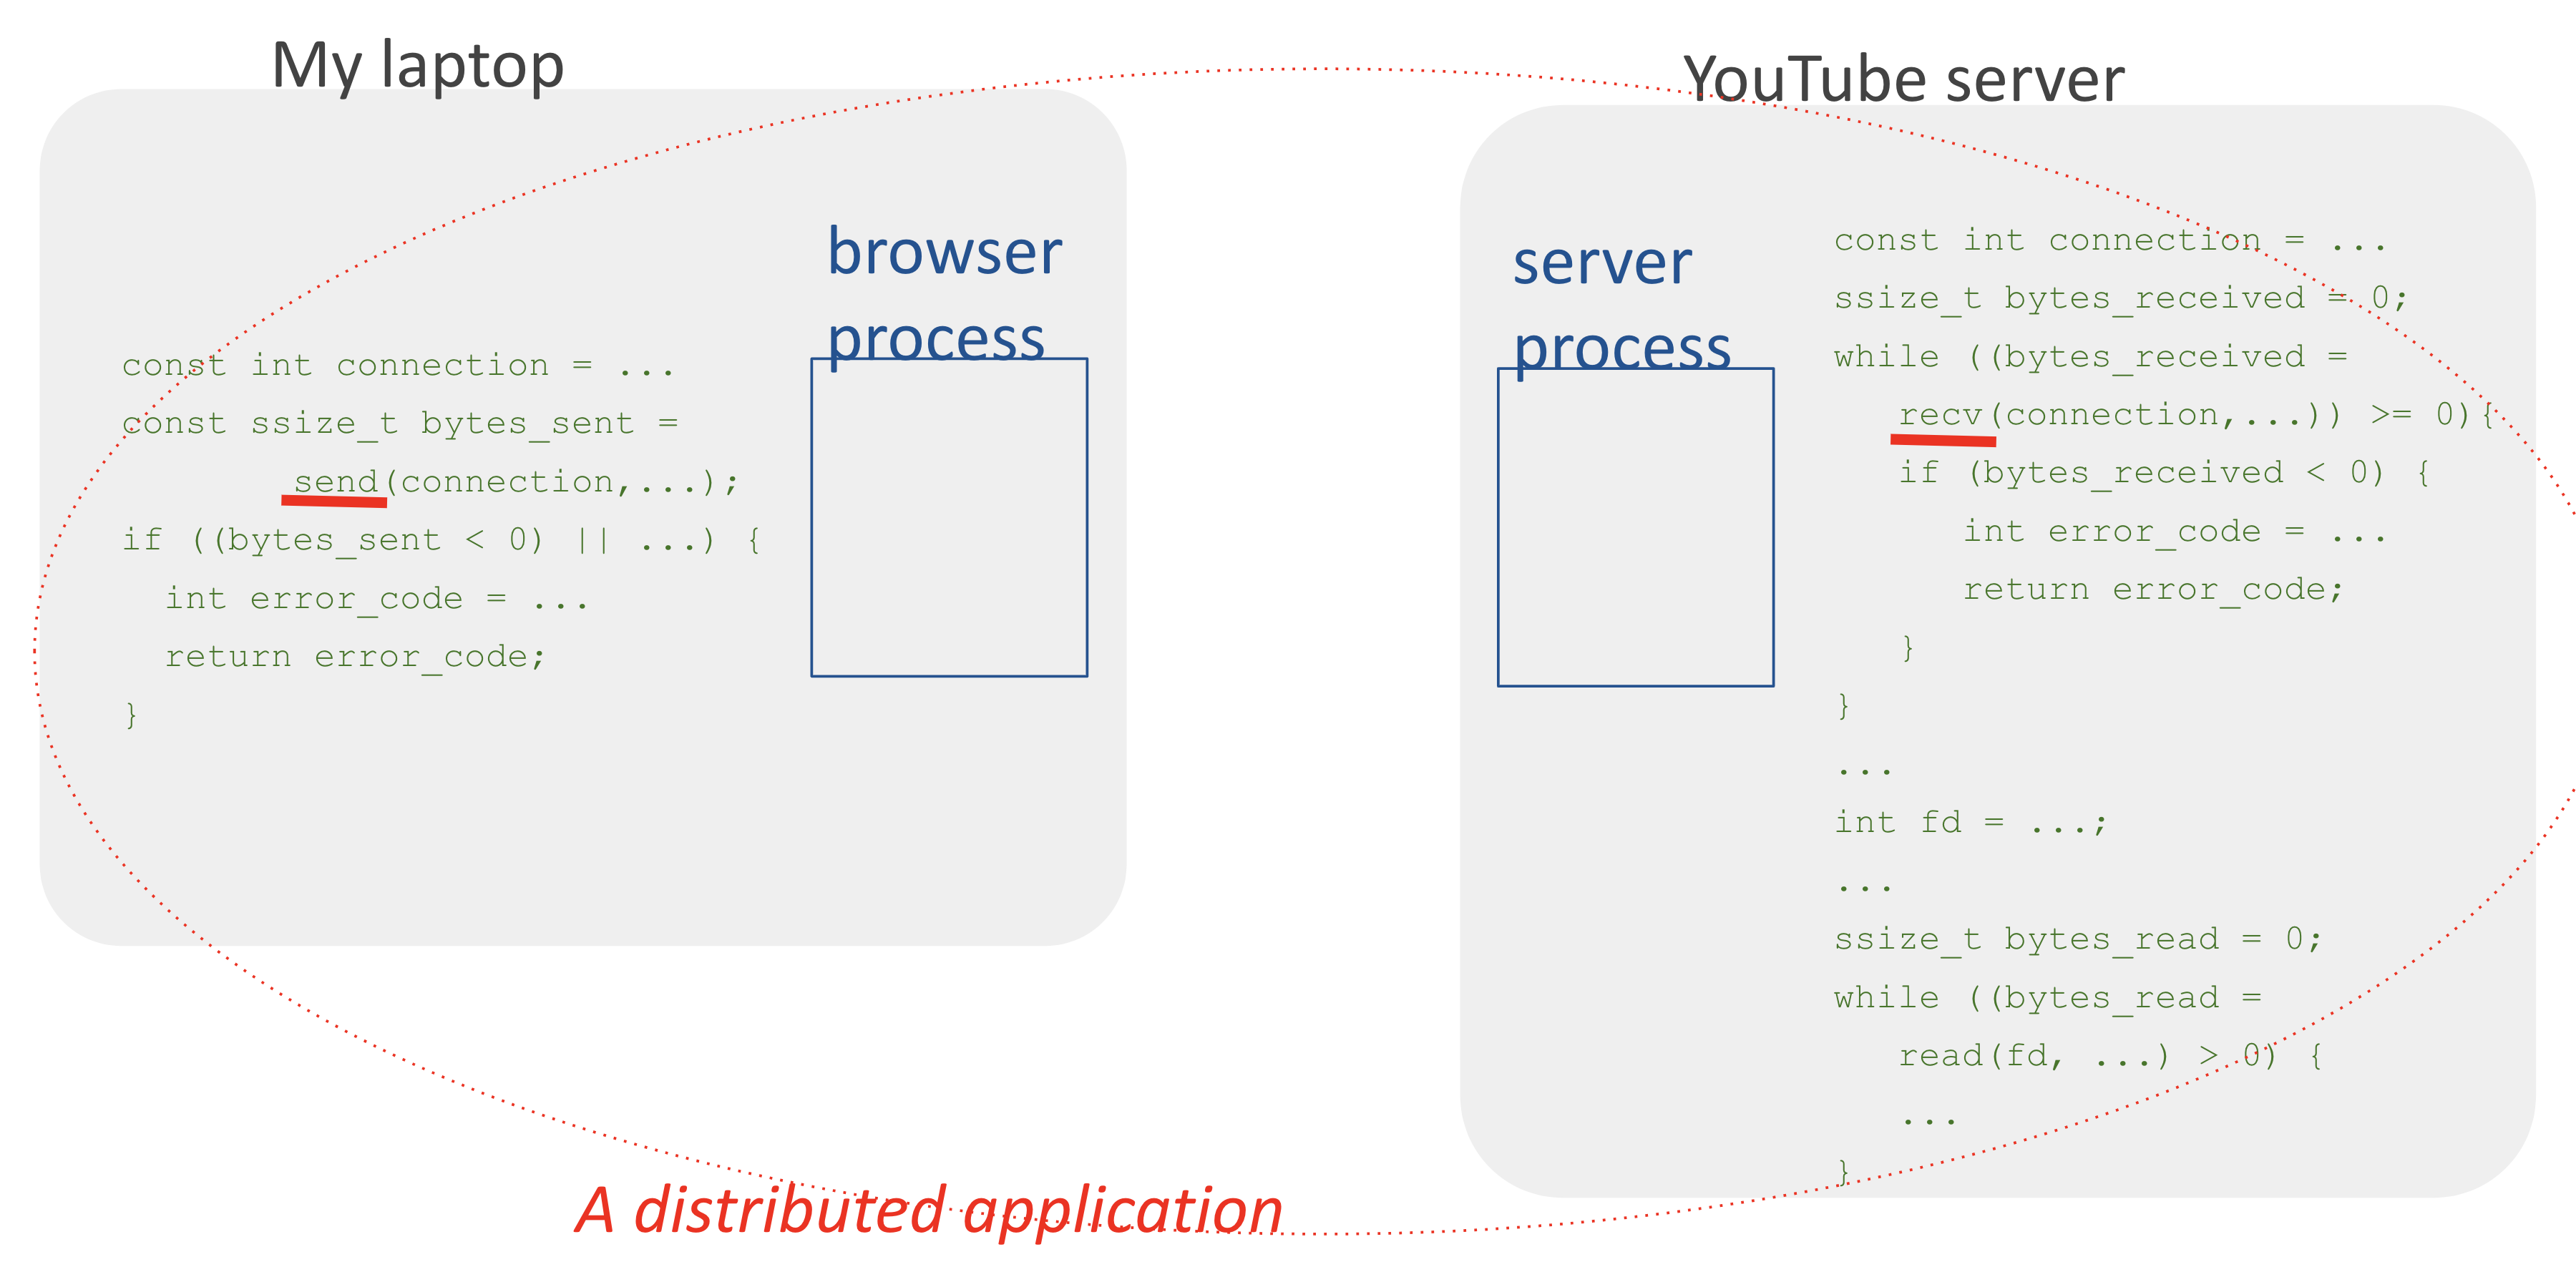
\includegraphics[width=0.95\textwidth]{chapters/L1/images/distributed.png}
\end{center}

%%%%%%%%%%%%%%%%%%%%%%%%%%%%%%%%%%%%%%%%%%%%%%%%%%%%%%%%%%%%%%%%%%%%%%
\newpage
\subsection{Communication Protocols}
For two processes running on different devices to work together, they must follow a predetermined set of rules known as a \textbf{communication protocol}. For example, a simple protocol might involve:
\begin{itemize}
  \item[-] One process sending “hello” and waiting for a “hello back.”
  \item[-] A subsequent request for a specific file (e.g., \texttt{xyz}) with the server responding with the file or an error message.
\end{itemize}
Much like human communication, these protocols ensure that both parties know what to expect, enabling effective interaction.

\begin{center}
  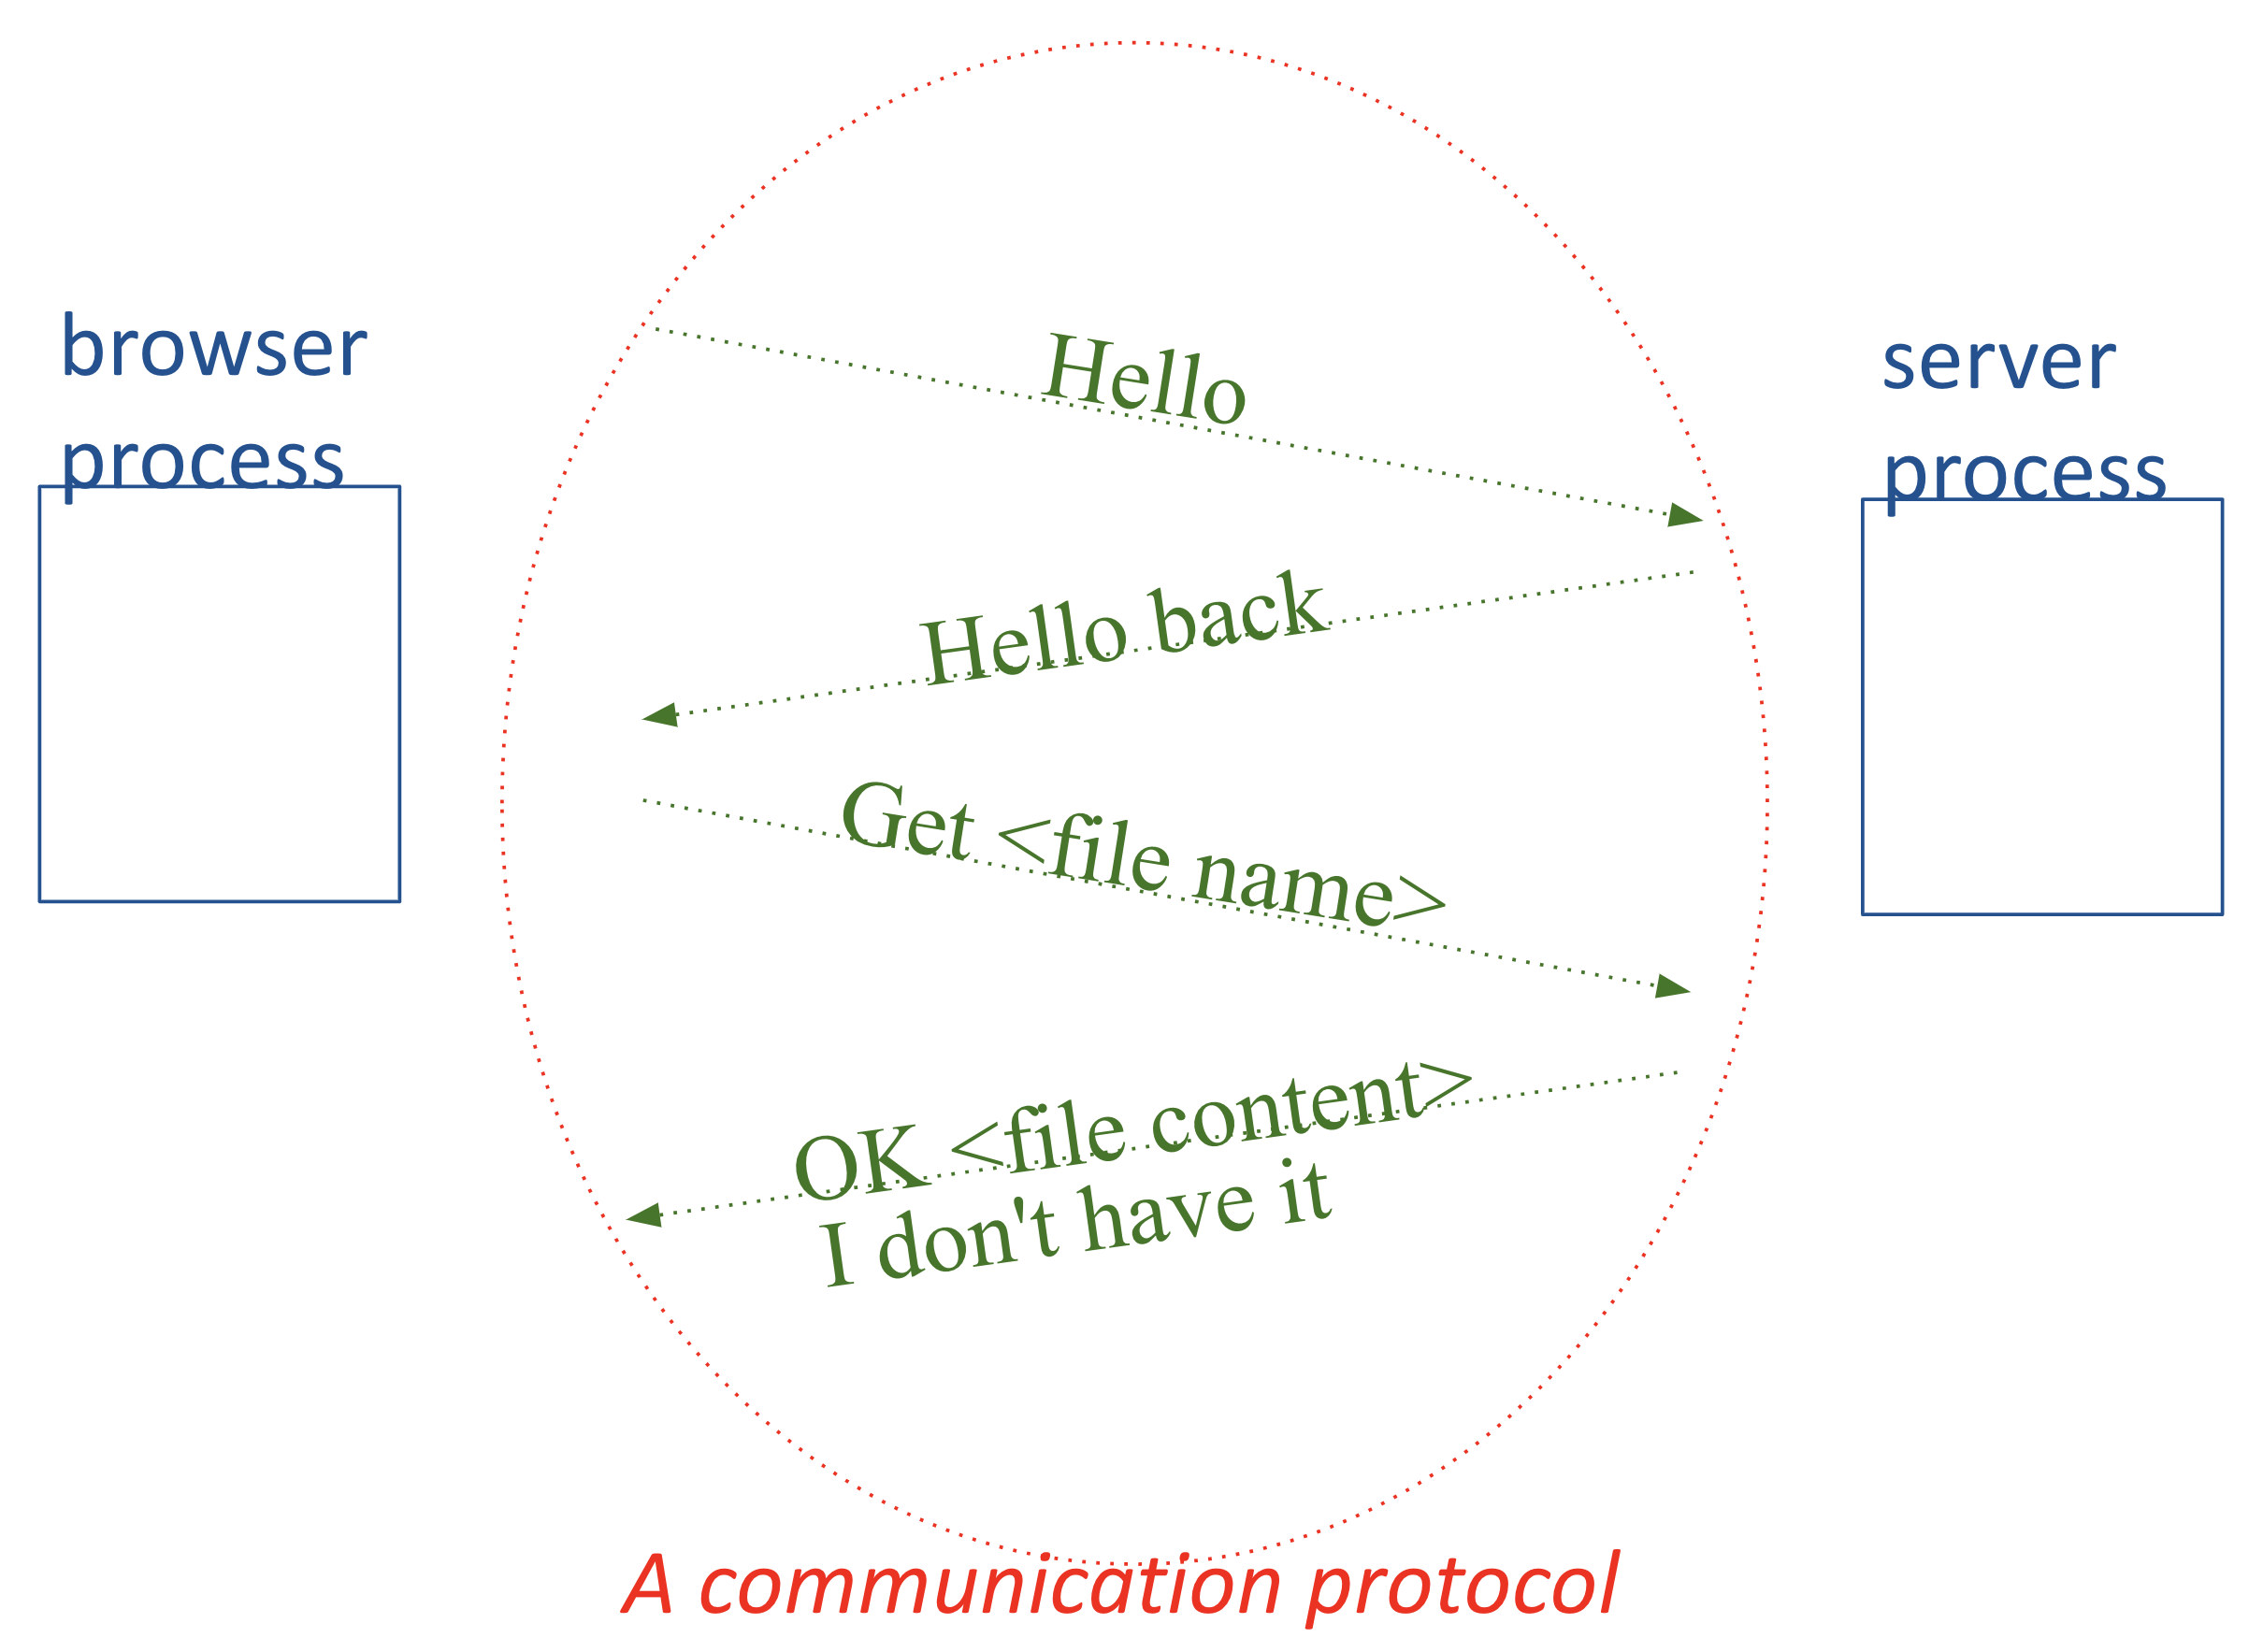
\includegraphics[width=0.45\textwidth]{chapters/L1/images/comm_prot.png}
\end{center}

%%%%%%%%%%%%%%%%%%%%%%%%%%%%%%%%%%%%%%%%%%%%%%%%%%%%%%%%%%%%%%%%%%%%%%
\subsection{Distributed Applications and APIs}

Distributed applications consist of separate pieces of code running as processes on different machines but working toward a common goal. These processes exchange messages over the Internet by following communication protocols.  
To simplify the development of these applications, developers use \emph{system calls} (or \textbf{syscalls}). Syscalls are special functions provided by the operating system that allow processes to access resources (e.g., network and storage) without needing to know the low-level details.

The set of syscalls available to an application forms its \textbf{Application Programming Interface} (API), abstracting away the complexities of resource management.

\begin{center}
  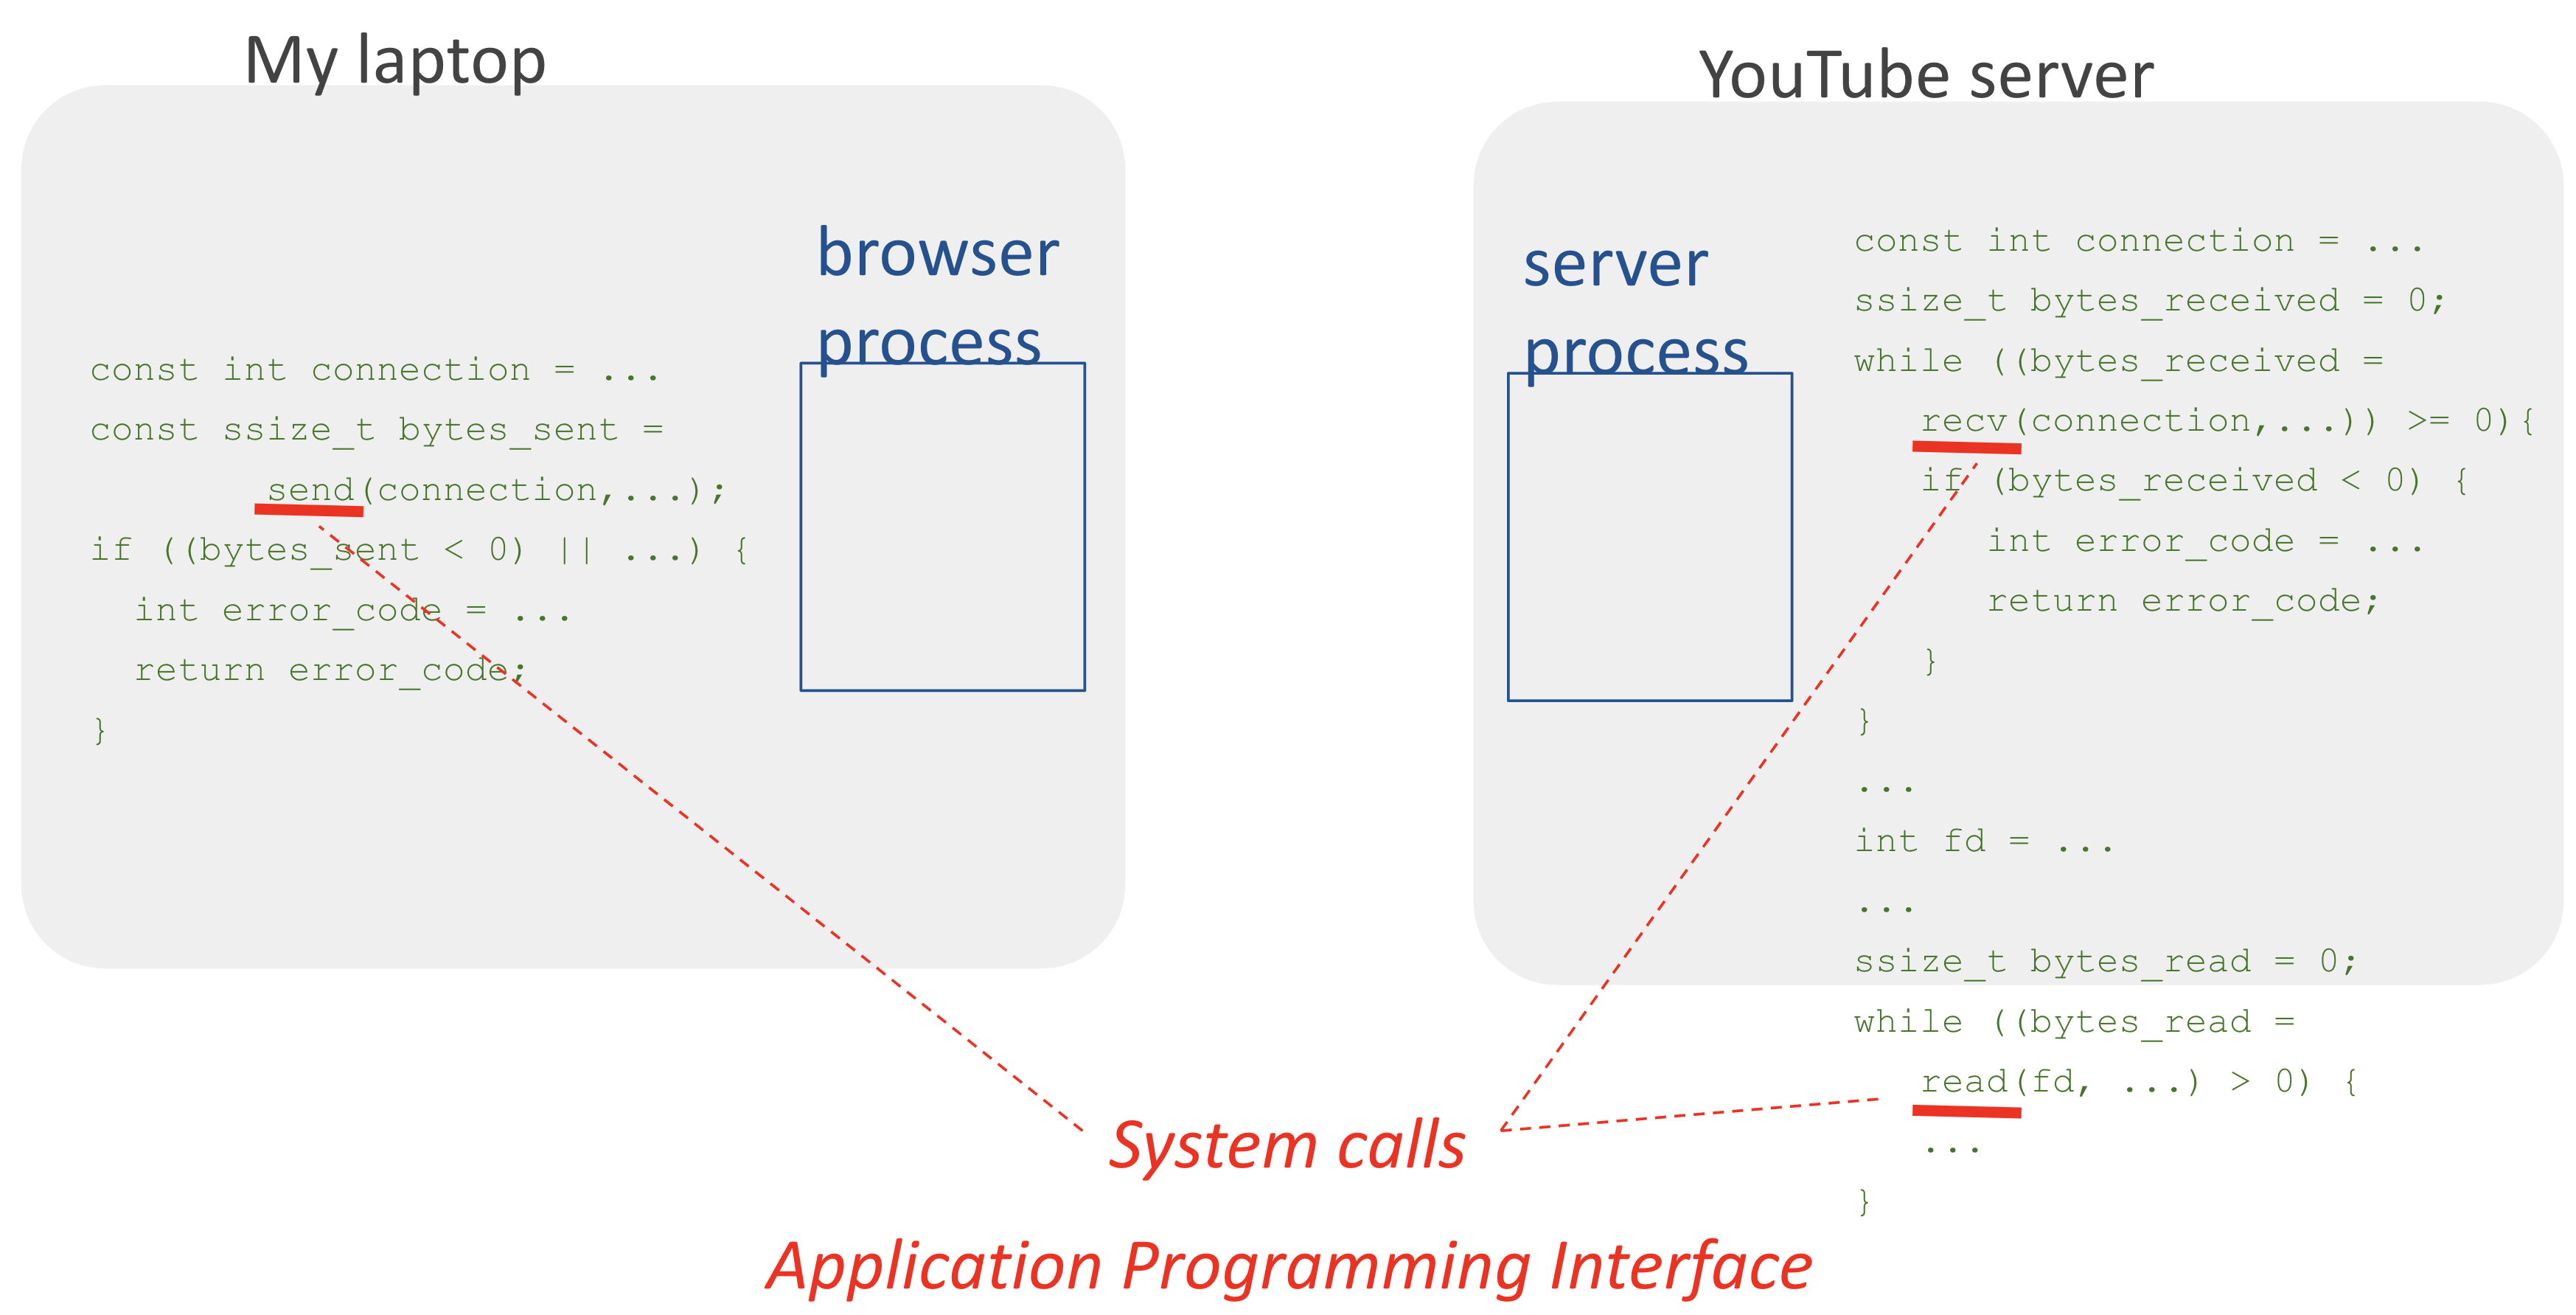
\includegraphics[width=0.85\textwidth]{chapters/L1/images/api.png}
\end{center}

%%%%%%%%%%%%%%%%%%%%%%%%%%%%%%%%%%%%%%%%%%%%%%%%%%%%%%%%%%%%%%%%%%%%%%
\vfill
\begin{definition}[Interface]
An \textbf{interface} is a set of rules that defines how different components communicate. For instance, when sending a letter via the postal system, one must follow specific rules (e.g., write the address and affix a stamp). This interface abstracts the complexities of the postal system so that users do not need to understand its internal operations.
\end{definition}

\begin{center}
  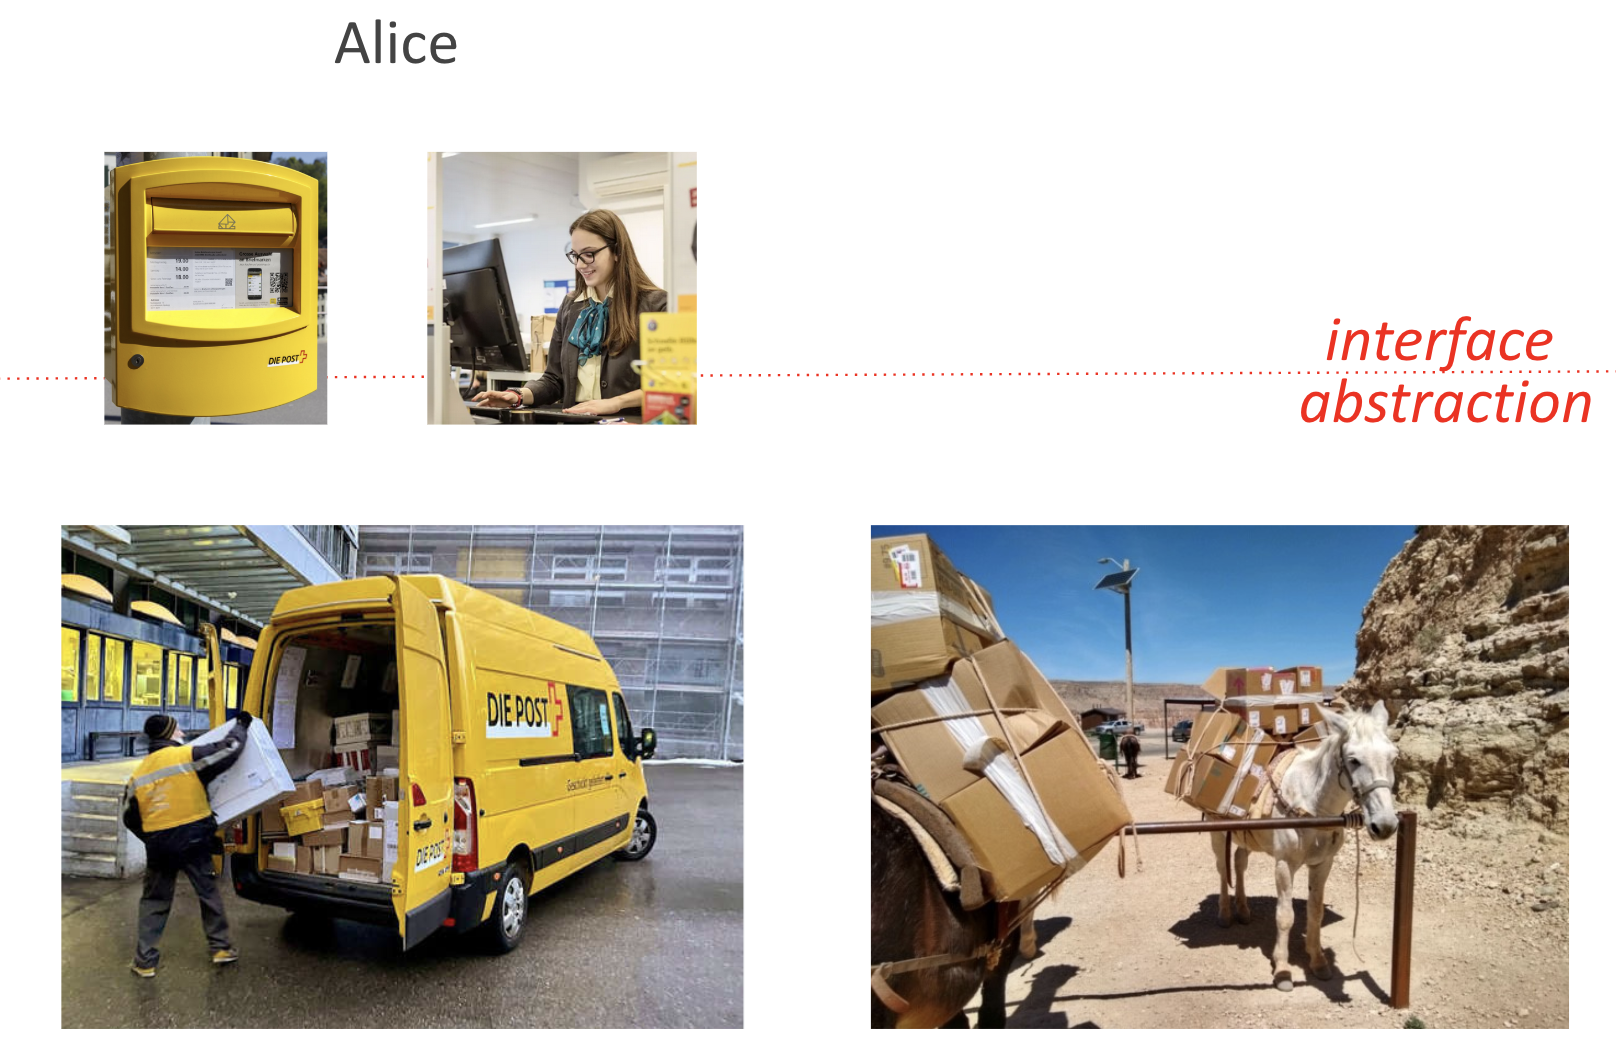
\includegraphics[width=0.65\textwidth]{chapters/L1/images/postal.png}
\end{center}
\vfill
%%%%%%%%%%%%%%%%%%%%%%%%%%%%%%%%%%%%%%%%%%%%%%%%%%%%%%%%%%%%%%%%%%%%%%
\subsection{System Calls (Syscalls)}

Syscalls form the interface between a process and external resources (like network and storage). They provide an abstraction of these resources, allowing a process to use them without knowing their intricate details. For example, when a process makes a syscall such as \texttt{send} or \texttt{recv}, the operating system’s network stack handles the details of the communication.

\begin{center}
  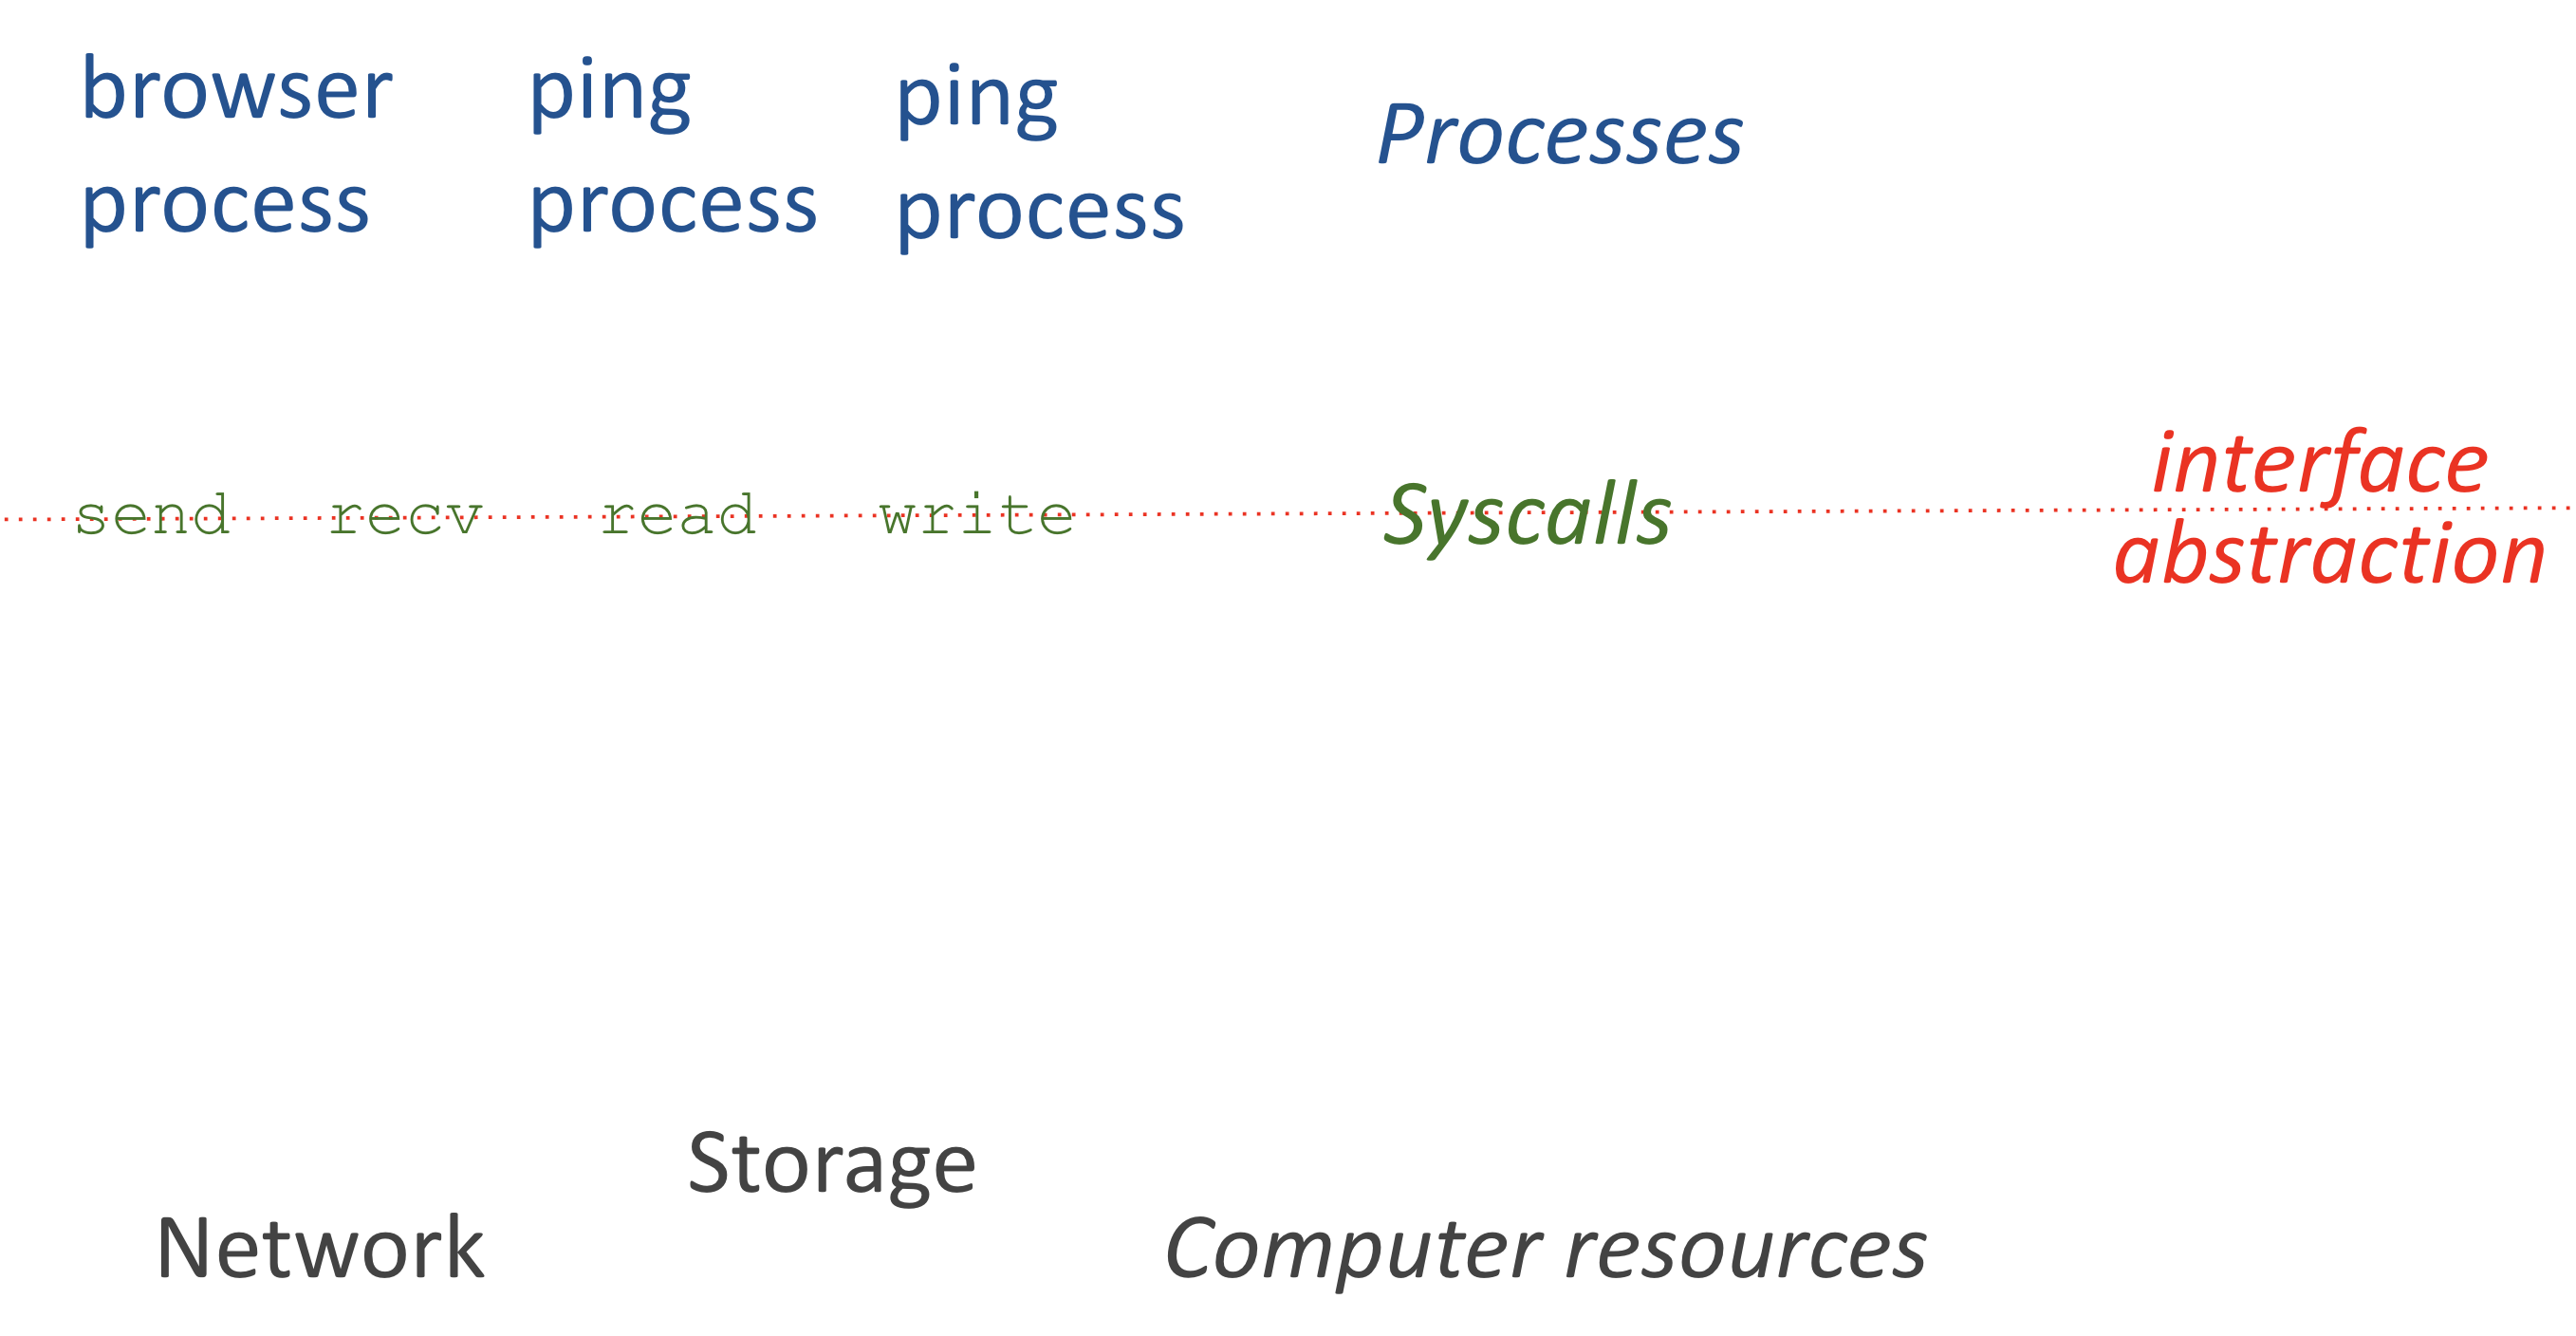
\includegraphics[width=0.65\textwidth]{chapters/L1/images/syscalls.png}
\end{center}
\vfill
\newpage
%%%%%%%%%%%%%%%%%%%%%%%%%%%%%%%%%%%%%%%%%%%%%%%%%%%%%%%%%%%%%%%%%%%%%%
\section{The Operating System}
Conceptually, the OS sits between running processes and the underlying hardware resources. It provides the syscall interface and handles tasks such as file system management and network communication. \\
\begin{minipage}{0.45\textwidth}
\begin{center}
  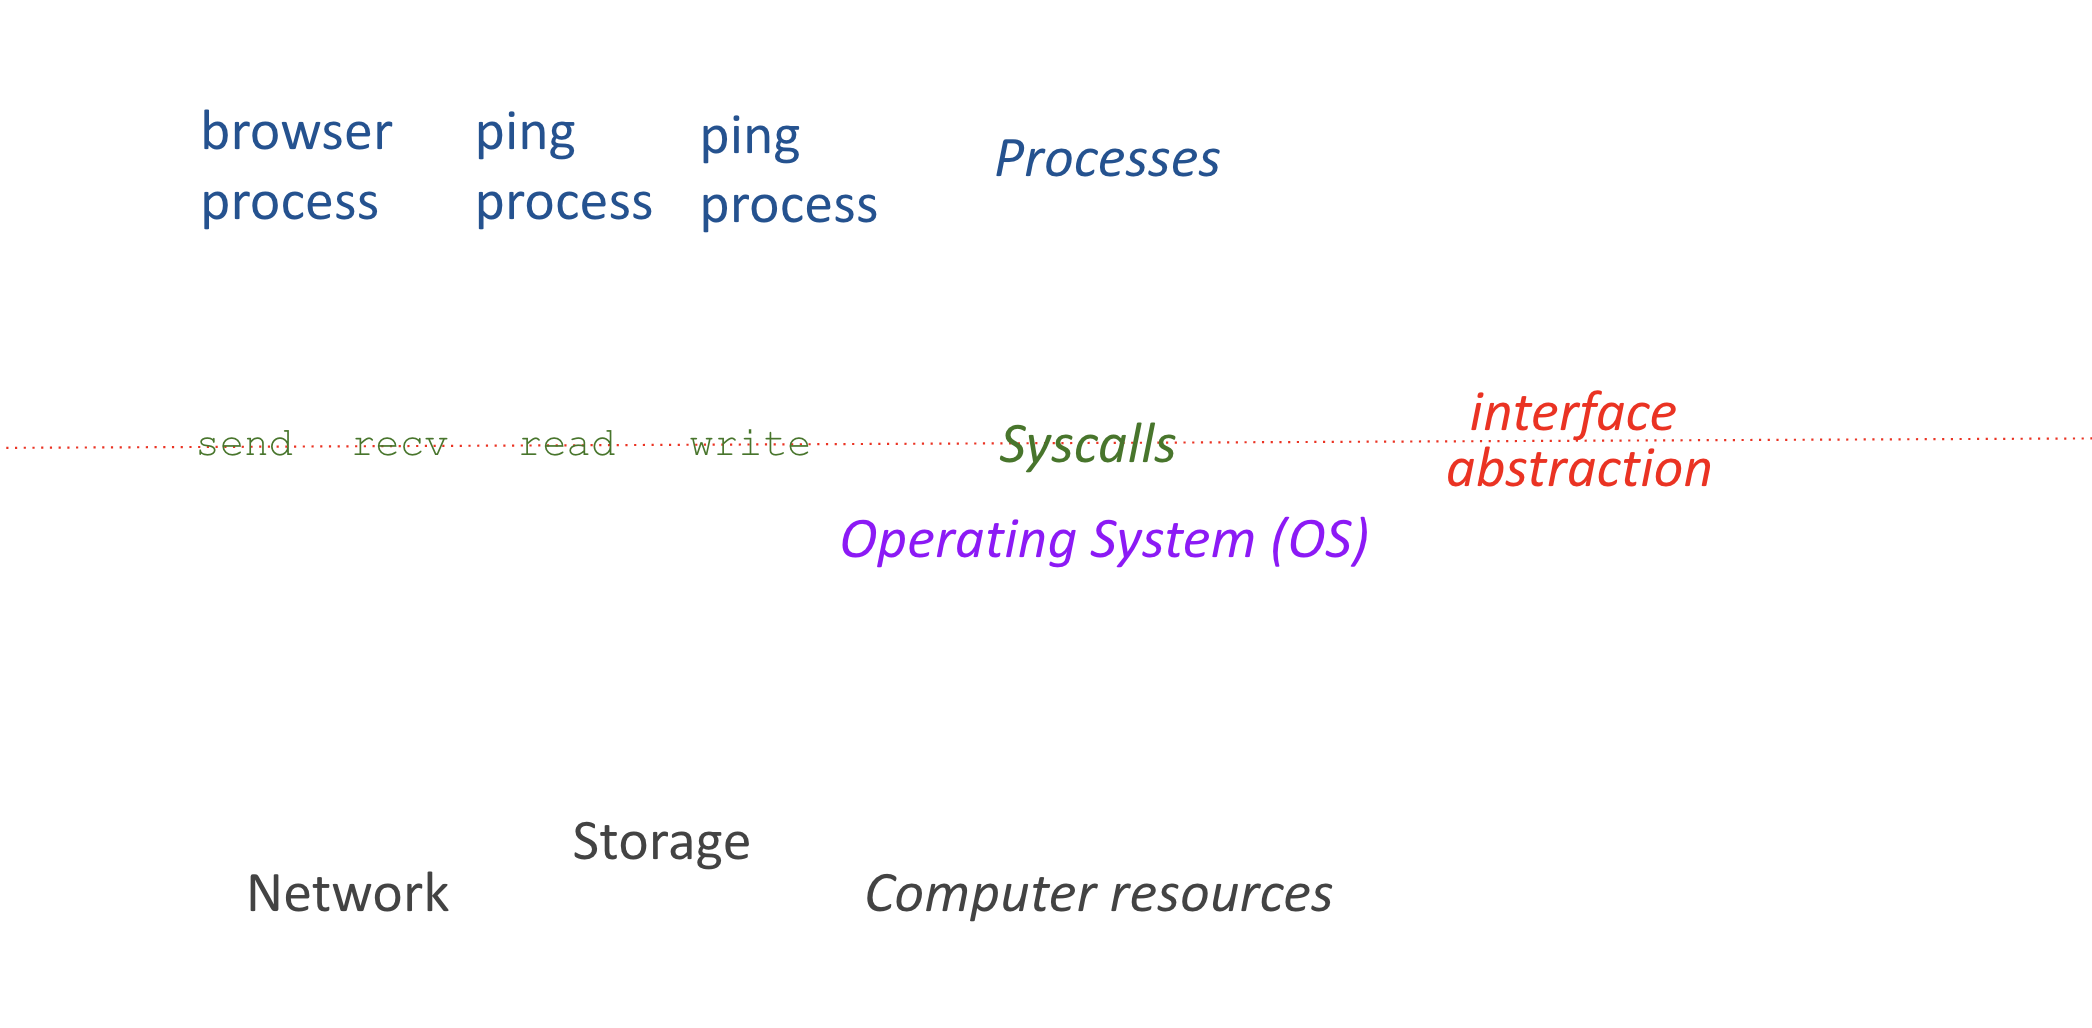
\includegraphics[width=1.15\textwidth]{chapters/L1/images/isa_os.png}
\end{center}
\end{minipage}
\hfill
\vline
\hfill
\begin{minipage}{0.45\textwidth}
\begin{center}
  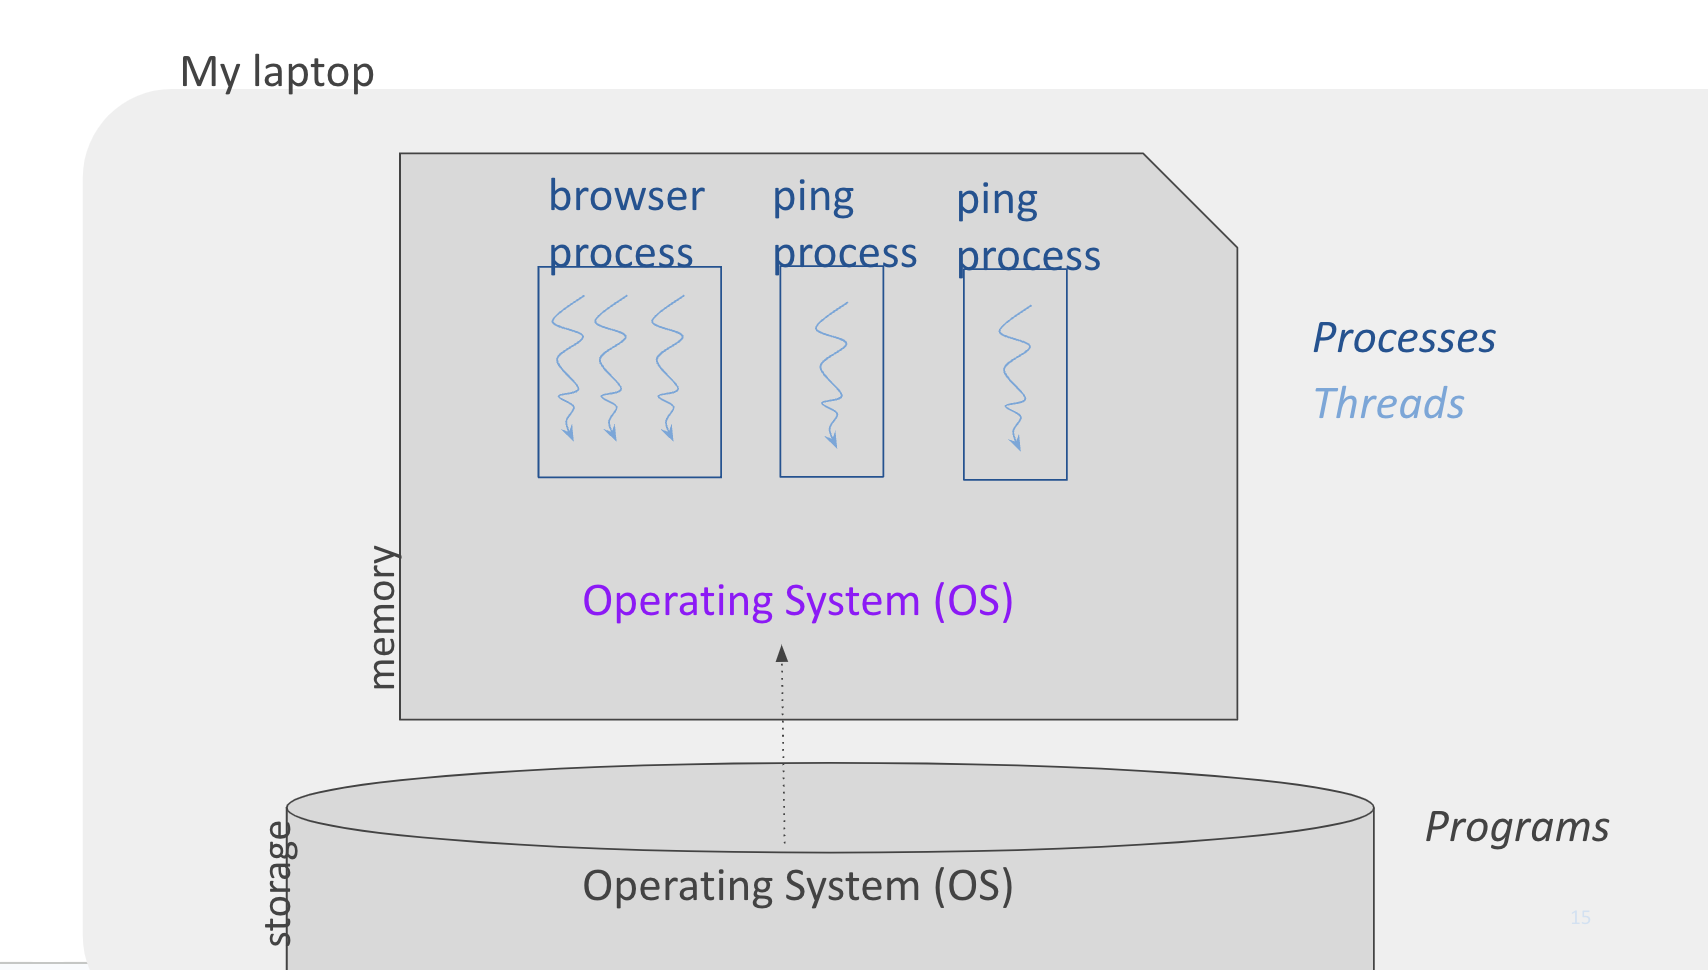
\includegraphics[width=1.15\textwidth]{chapters/L1/images/os.png}
\end{center}
\end{minipage}

\subsection{Example: Execution When Fetching a Video from YouTube}
When you click a YouTube link, the following sequence of events occurs:
\begin{enumerate}
  \item Your trackpad detects the click and notifies the OS.
  \item The OS identifies that the click occurred within the web browser window and alerts the corresponding process.
  \item The browser process initiates a chain of events that eventually fetches and displays the video.
\end{enumerate}

\begin{center}
  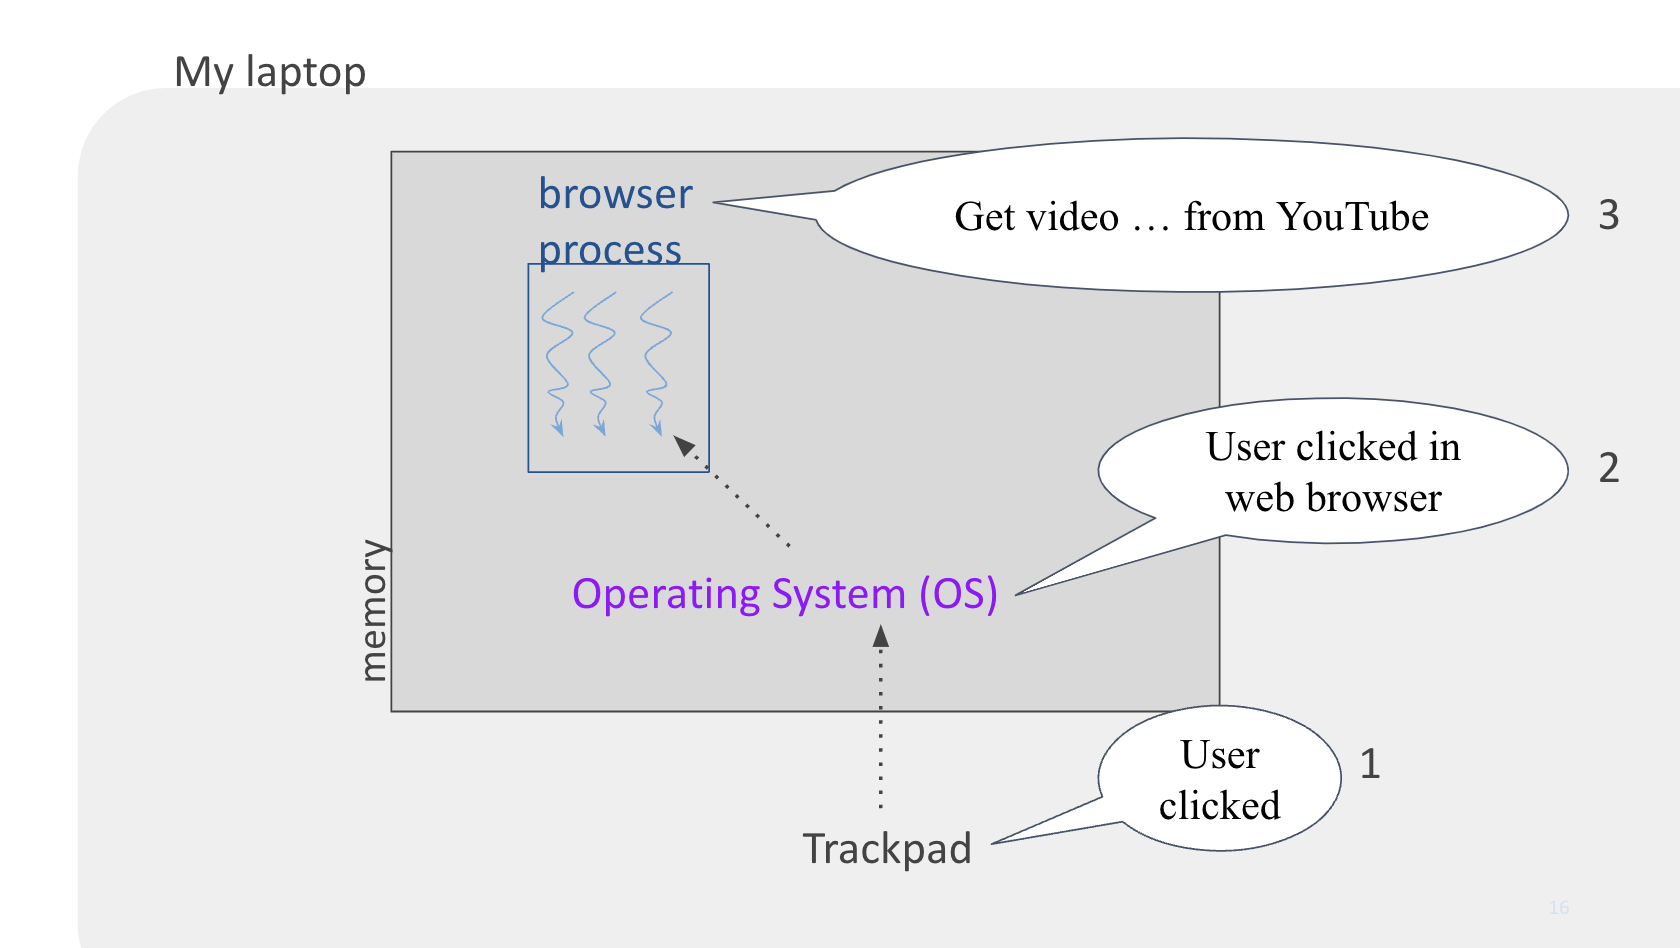
\includegraphics[width=0.85\textwidth]{chapters/L1/images/os_youtube.png}
\end{center}

\newpage
%%%%%%%%%%%%%%%%%%%%%%%%%%%%%%%%%%%%%%%%%%%%%%%%%%%%%%%%%%%%%%%%%%%%%%
\section{Program and ISA}
\subsection{Program}
A \textbf{program} is a set of instructions written by a human in a high-level programming language (such as C, Java, or Python) that implements an algorithm. When compiled, a program is translated into an \emph{executable} (or binary) that the CPU can run. The executable is expressed in the language defined by the computer's \textbf{Instruction Set Architecture} (ISA).

\begin{center}
  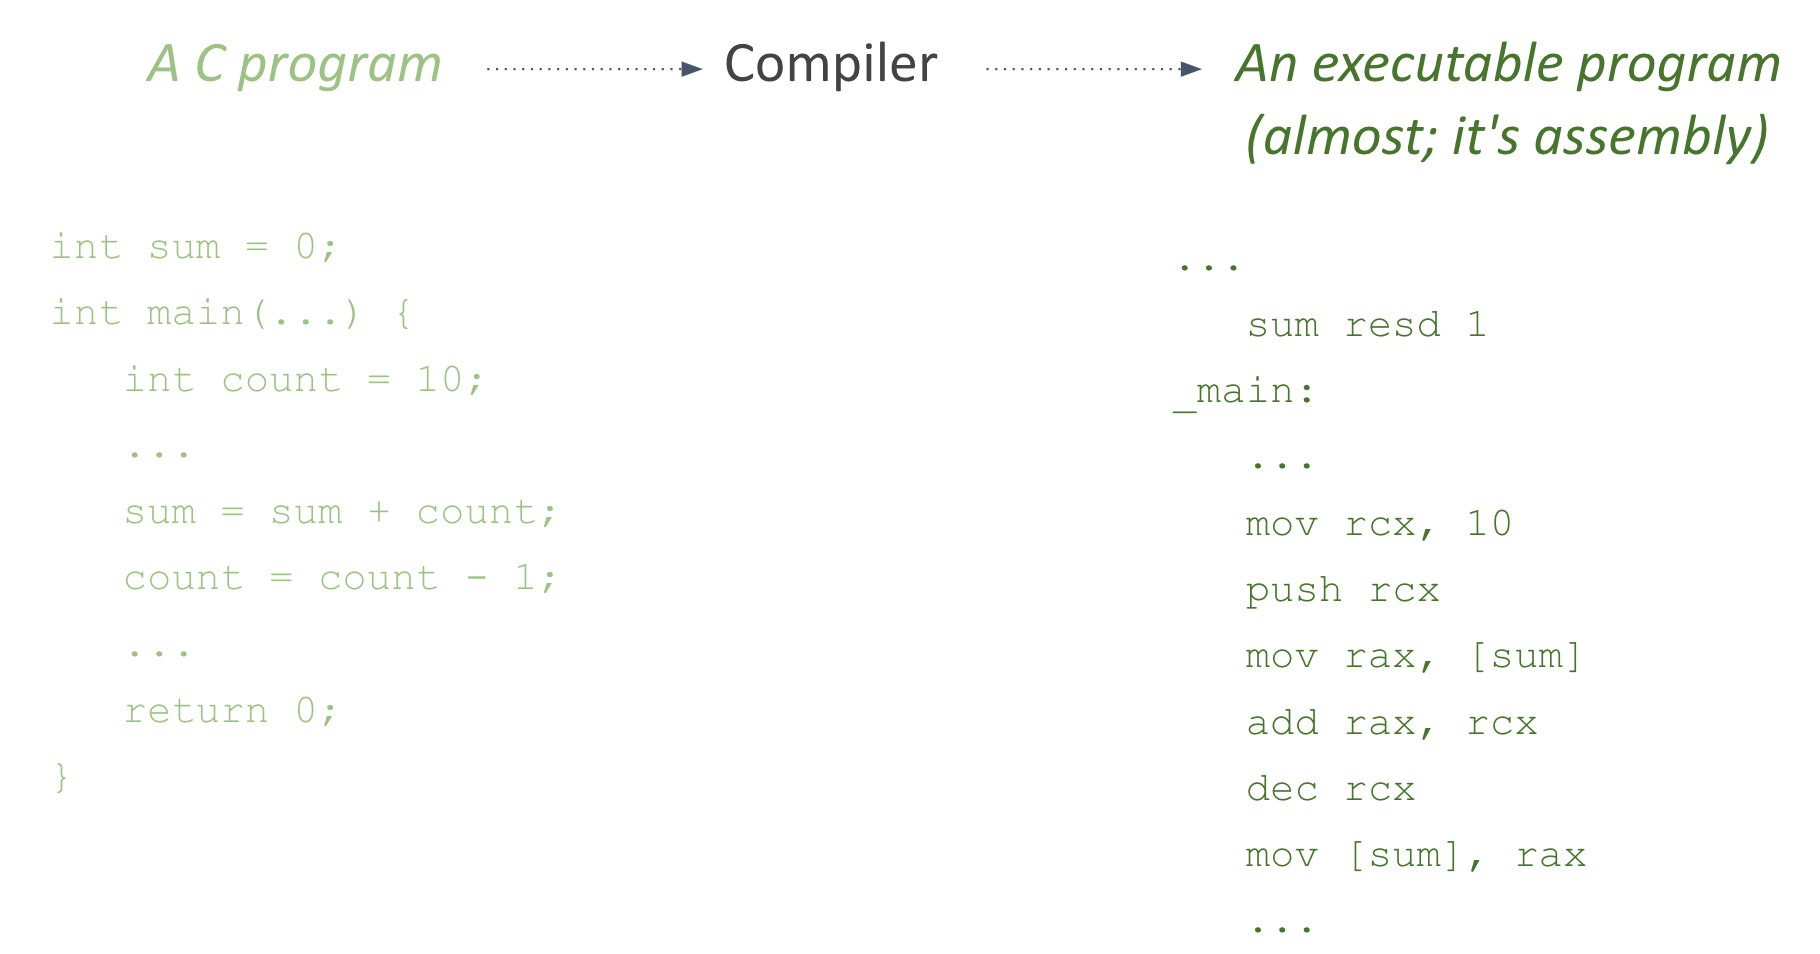
\includegraphics[width=0.75\textwidth]{chapters/L1/images/program.png}
\end{center}

\begin{minipage}{0.45\textwidth}
\begin{definition}[ISA]
The \textbf{Instruction Set Architecture} (ISA) is the set of all instructions that a CPU can understand and execute. It forms an interface between the compiler (which translates high-level code into machine code) and the CPU.
\end{definition}
\end{minipage}
\hfill
\vline
\hfill
\begin{minipage}{0.45\textwidth}
\begin{center}
  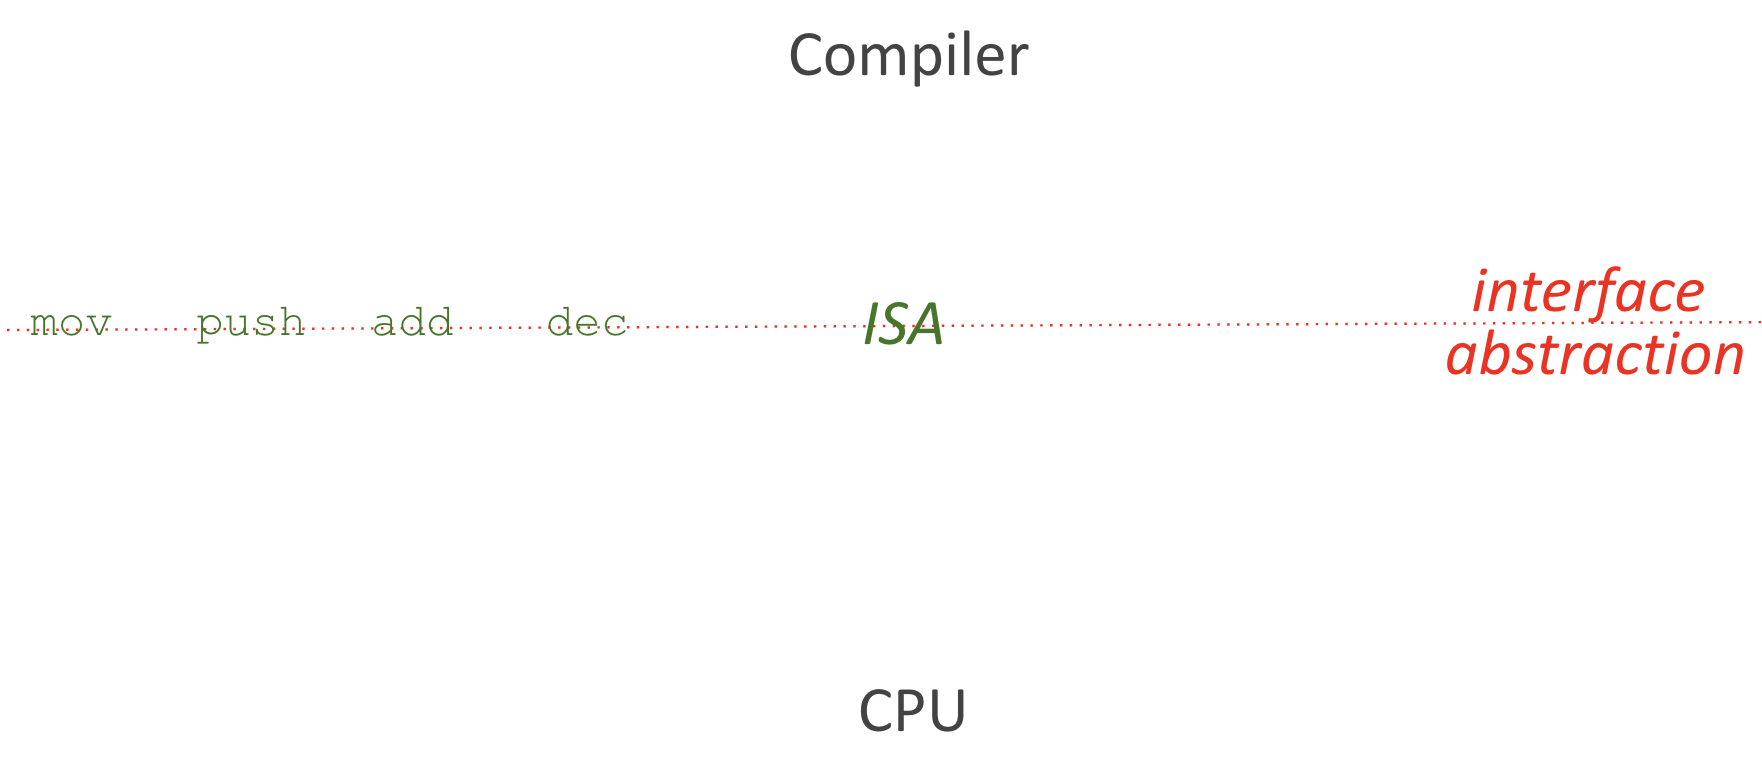
\includegraphics[width=1.25\textwidth]{chapters/L1/images/isa.png}
\end{center}
\end{minipage}\\
\vfill
\begin{definition}[Von Neumann Architecture]
The vast majority of computers today follow the \textbf{Von Neumann architecture}, which is characterized by a single main memory that holds both data and instructions.

\begin{center}
  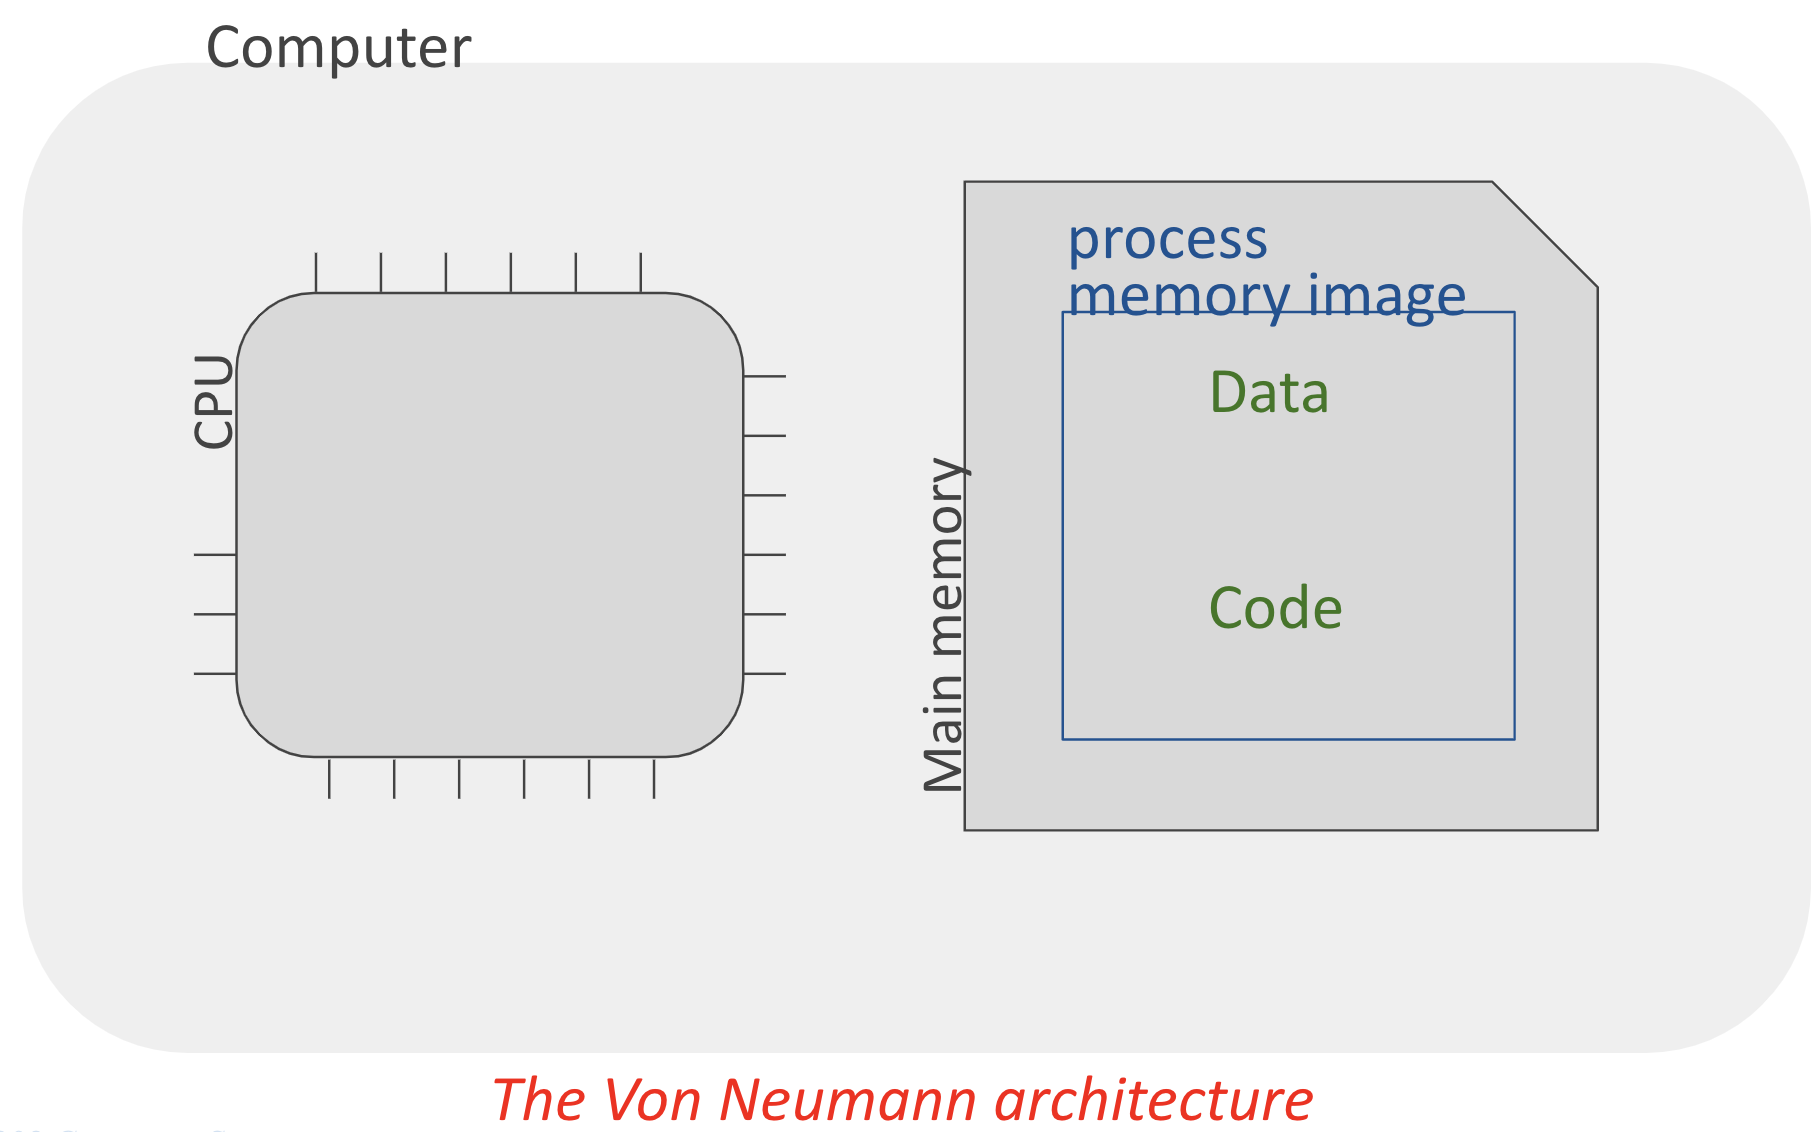
\includegraphics[width=0.55\textwidth]{chapters/L1/images/von.png}
\end{center}
\end{definition}

%%%%%%%%%%%%%%%%%%%%%%%%%%%%%%%%%%%%%%%%%%%%%%%%%%%%%%%%%%%%%%%%%%%%%%
\begin{definition}[CPU Frequency]
A CPU’s frequency indicates how many cycles it can perform in one second. For example, a 4.05~GHz CPU performs 4.05 billion cycles per second. In this context, a \textbf{cycle} is the minimum time needed for the CPU to complete an operation or for a result to become ready.\\
\vspace{0.5em}
{\textbf{Question:} What is the meaning of the Hz metric?}\\[0.5em]
\textbf{Answer:} Hertz (Hz) measures the number of cycles per second.
\vspace{0.5em}
{\textbf{Question:} In the context of a CPU, what is a cycle?}\\[0.5em]
\textbf{Answer:} A cycle is the minimum unit of time required for the CPU to produce a result from executing an instruction.
\end{definition}


%%%%%%%%%%%%%%%%%%%%%%%%%%%%%%%%%%%%%%%%%%%%%%%%%%%%%%%%%%%%%%%%%%%%%%
\section{Frequency Imbalance and CPU Caching}

Modern systems exhibit a \emph{frequency imbalance} between the CPU and main memory. While the CPU might complete an instruction in approximately 1~nsec, accessing data from DRAM typically takes 50–150~nsec. As a result, the CPU can spend a significant amount of time idle, waiting for data.

\begin{center}
  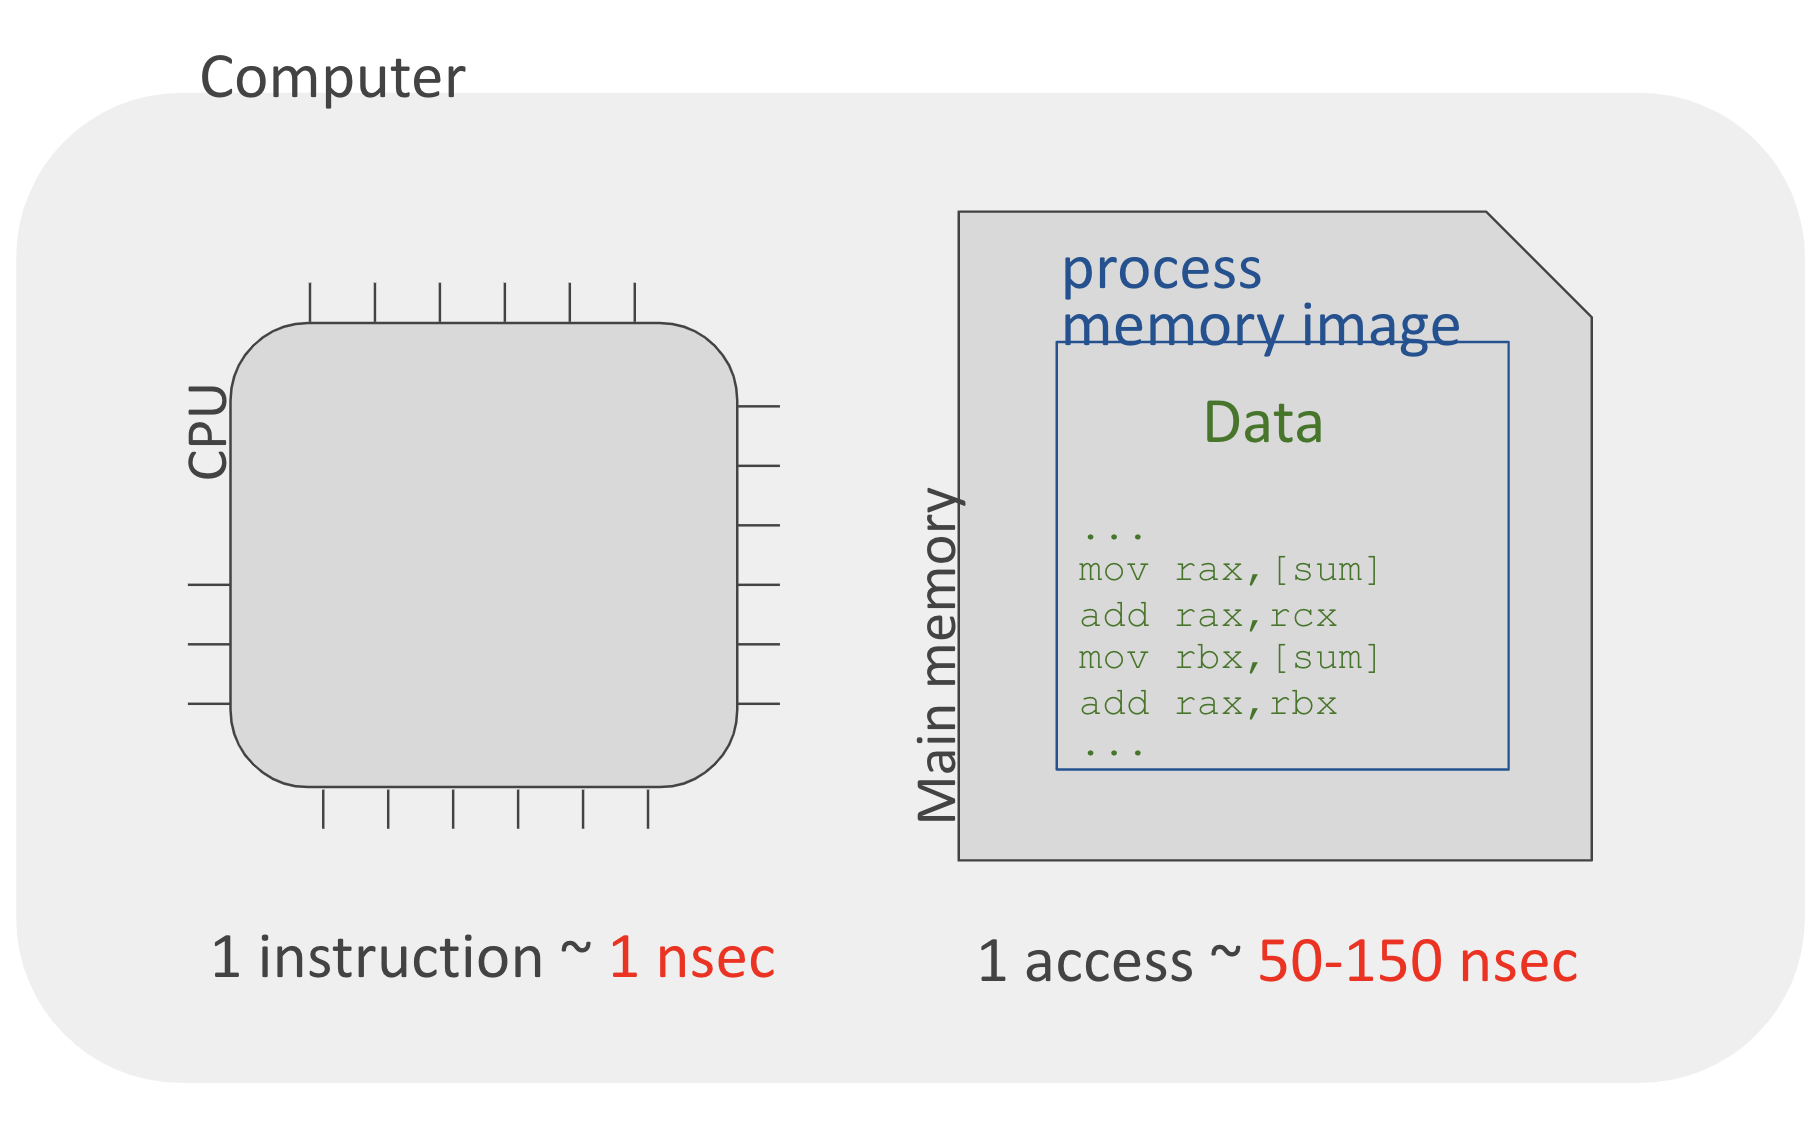
\includegraphics[width=0.65\textwidth]{chapters/L1/images/imbalance.png}
\end{center}

\vspace{0.5em}
{\textbf{Question:} How can we improve the efficiency of a system with such a frequency imbalance?}\\[0.5em]
\textbf{Answer:} We can improve efficiency by using caching. A small, fast memory (the CPU cache) stores recently accessed data so that subsequent accesses are much faster.
\newpage
\subsection{CPU Caching}
CPU caching adds a small amount of high-speed memory inside the CPU. When data is requested, the cache is checked first. If the data is already in the cache (a cache hit), the CPU retrieves it quickly. Otherwise (a cache miss), the data is fetched from the slower main memory and stored in the cache for future accesses.

\begin{center}
  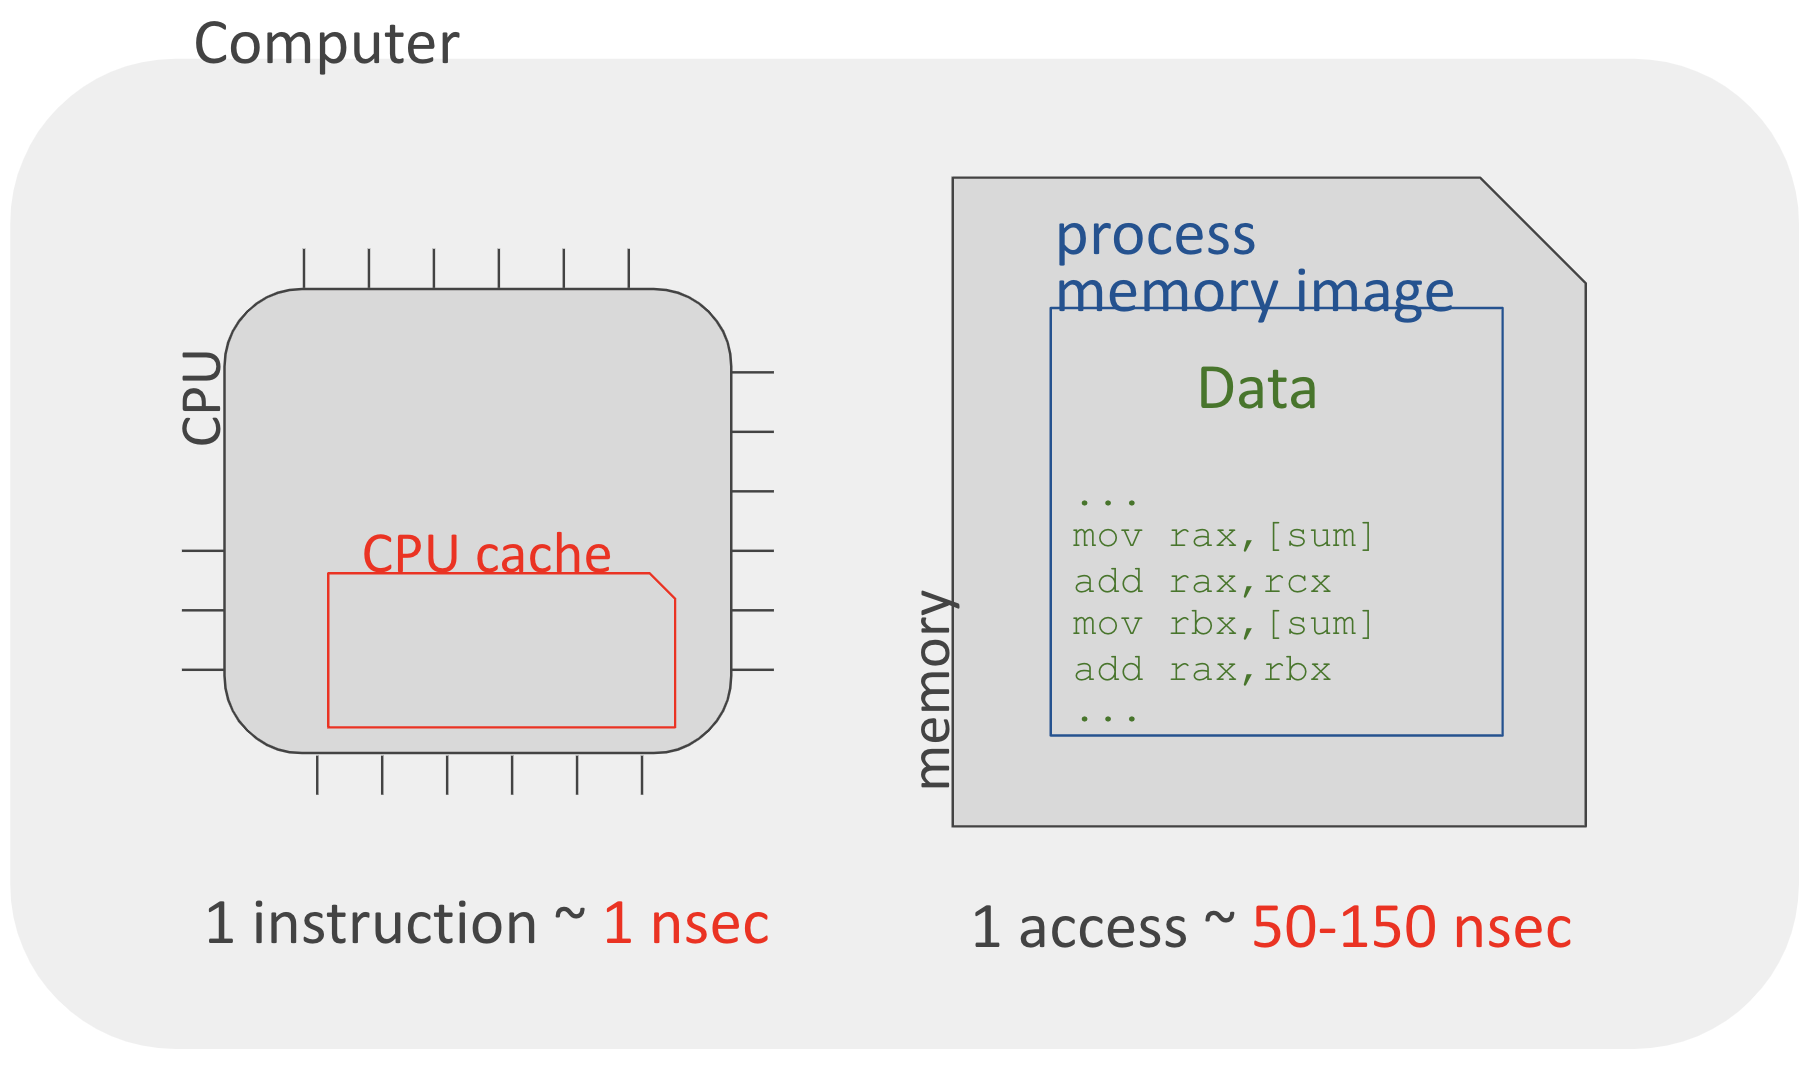
\includegraphics[width=0.65\textwidth]{chapters/L1/images/cache.png}
\end{center}

%%%%%%%%%%%%%%%%%%%%%%%%%%%%%%%%%%%%%%%%%%%%%%%%%%%%%%%%%%%%%%%%%%%%%%
\section{Memory Accesses vs. I/O}

\subsection{Memory Accesses}
When a process reads or writes data in main memory, it uses fast CPU instructions (load/store). These operations are efficient and do not interrupt the normal flow of the process.

\subsection{Back to YouTube Fetching: System Calls in Action}

Returning to our YouTube example, when the browser process calls a \texttt{send} syscall to request a video, the CPU stops executing the browser’s code and switches to executing the more privileged code in the OS. This is because accessing external resources (network or storage) requires a syscall.

\begin{center}
  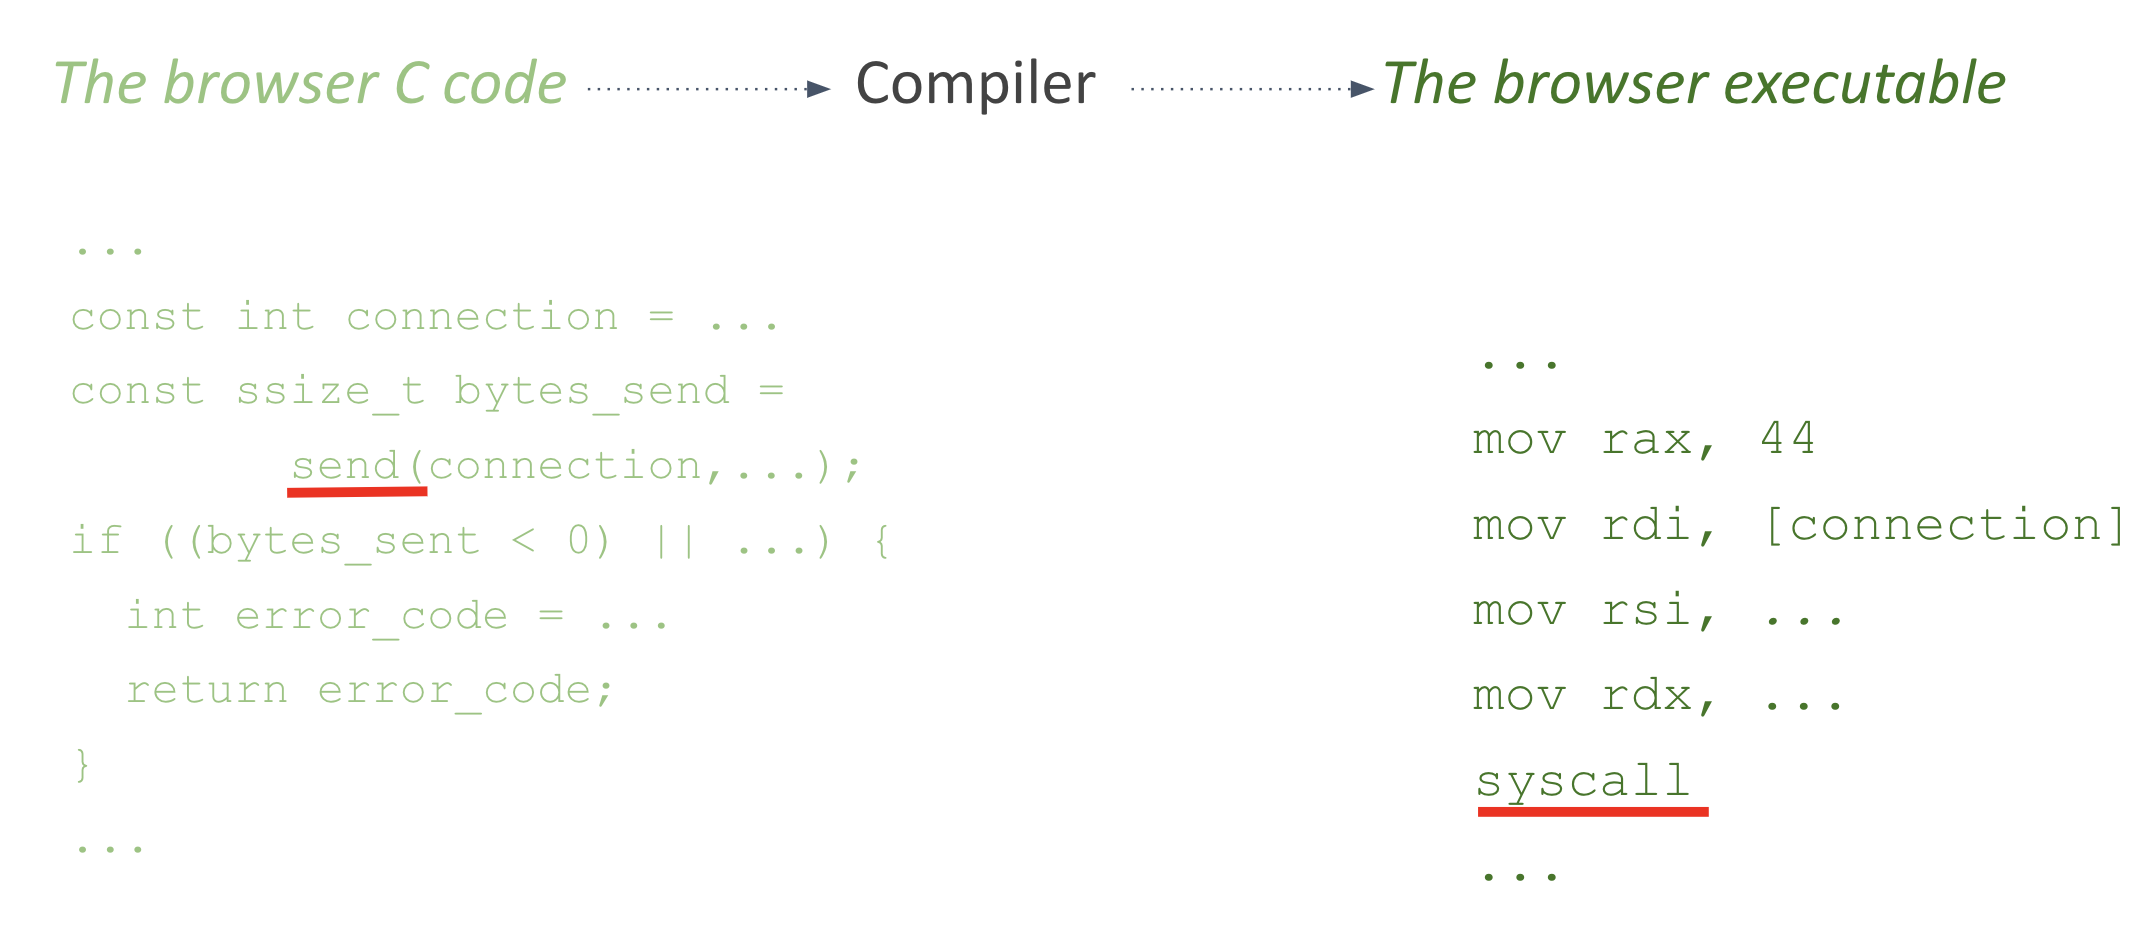
\includegraphics[width=0.85\textwidth]{chapters/L1/images/syscalls2.png}
\end{center}
\newpage
\subsection{Mixing Interfaces}
When a process makes a syscall for network communication (such as \texttt{send} or \texttt{recv}), the CPU transitions from running the process’s code to running the OS code associated with the network stack. This is an example of mixing different interfaces: the process interface (its own code) and the OS interface (syscalls).
\begin{center}
  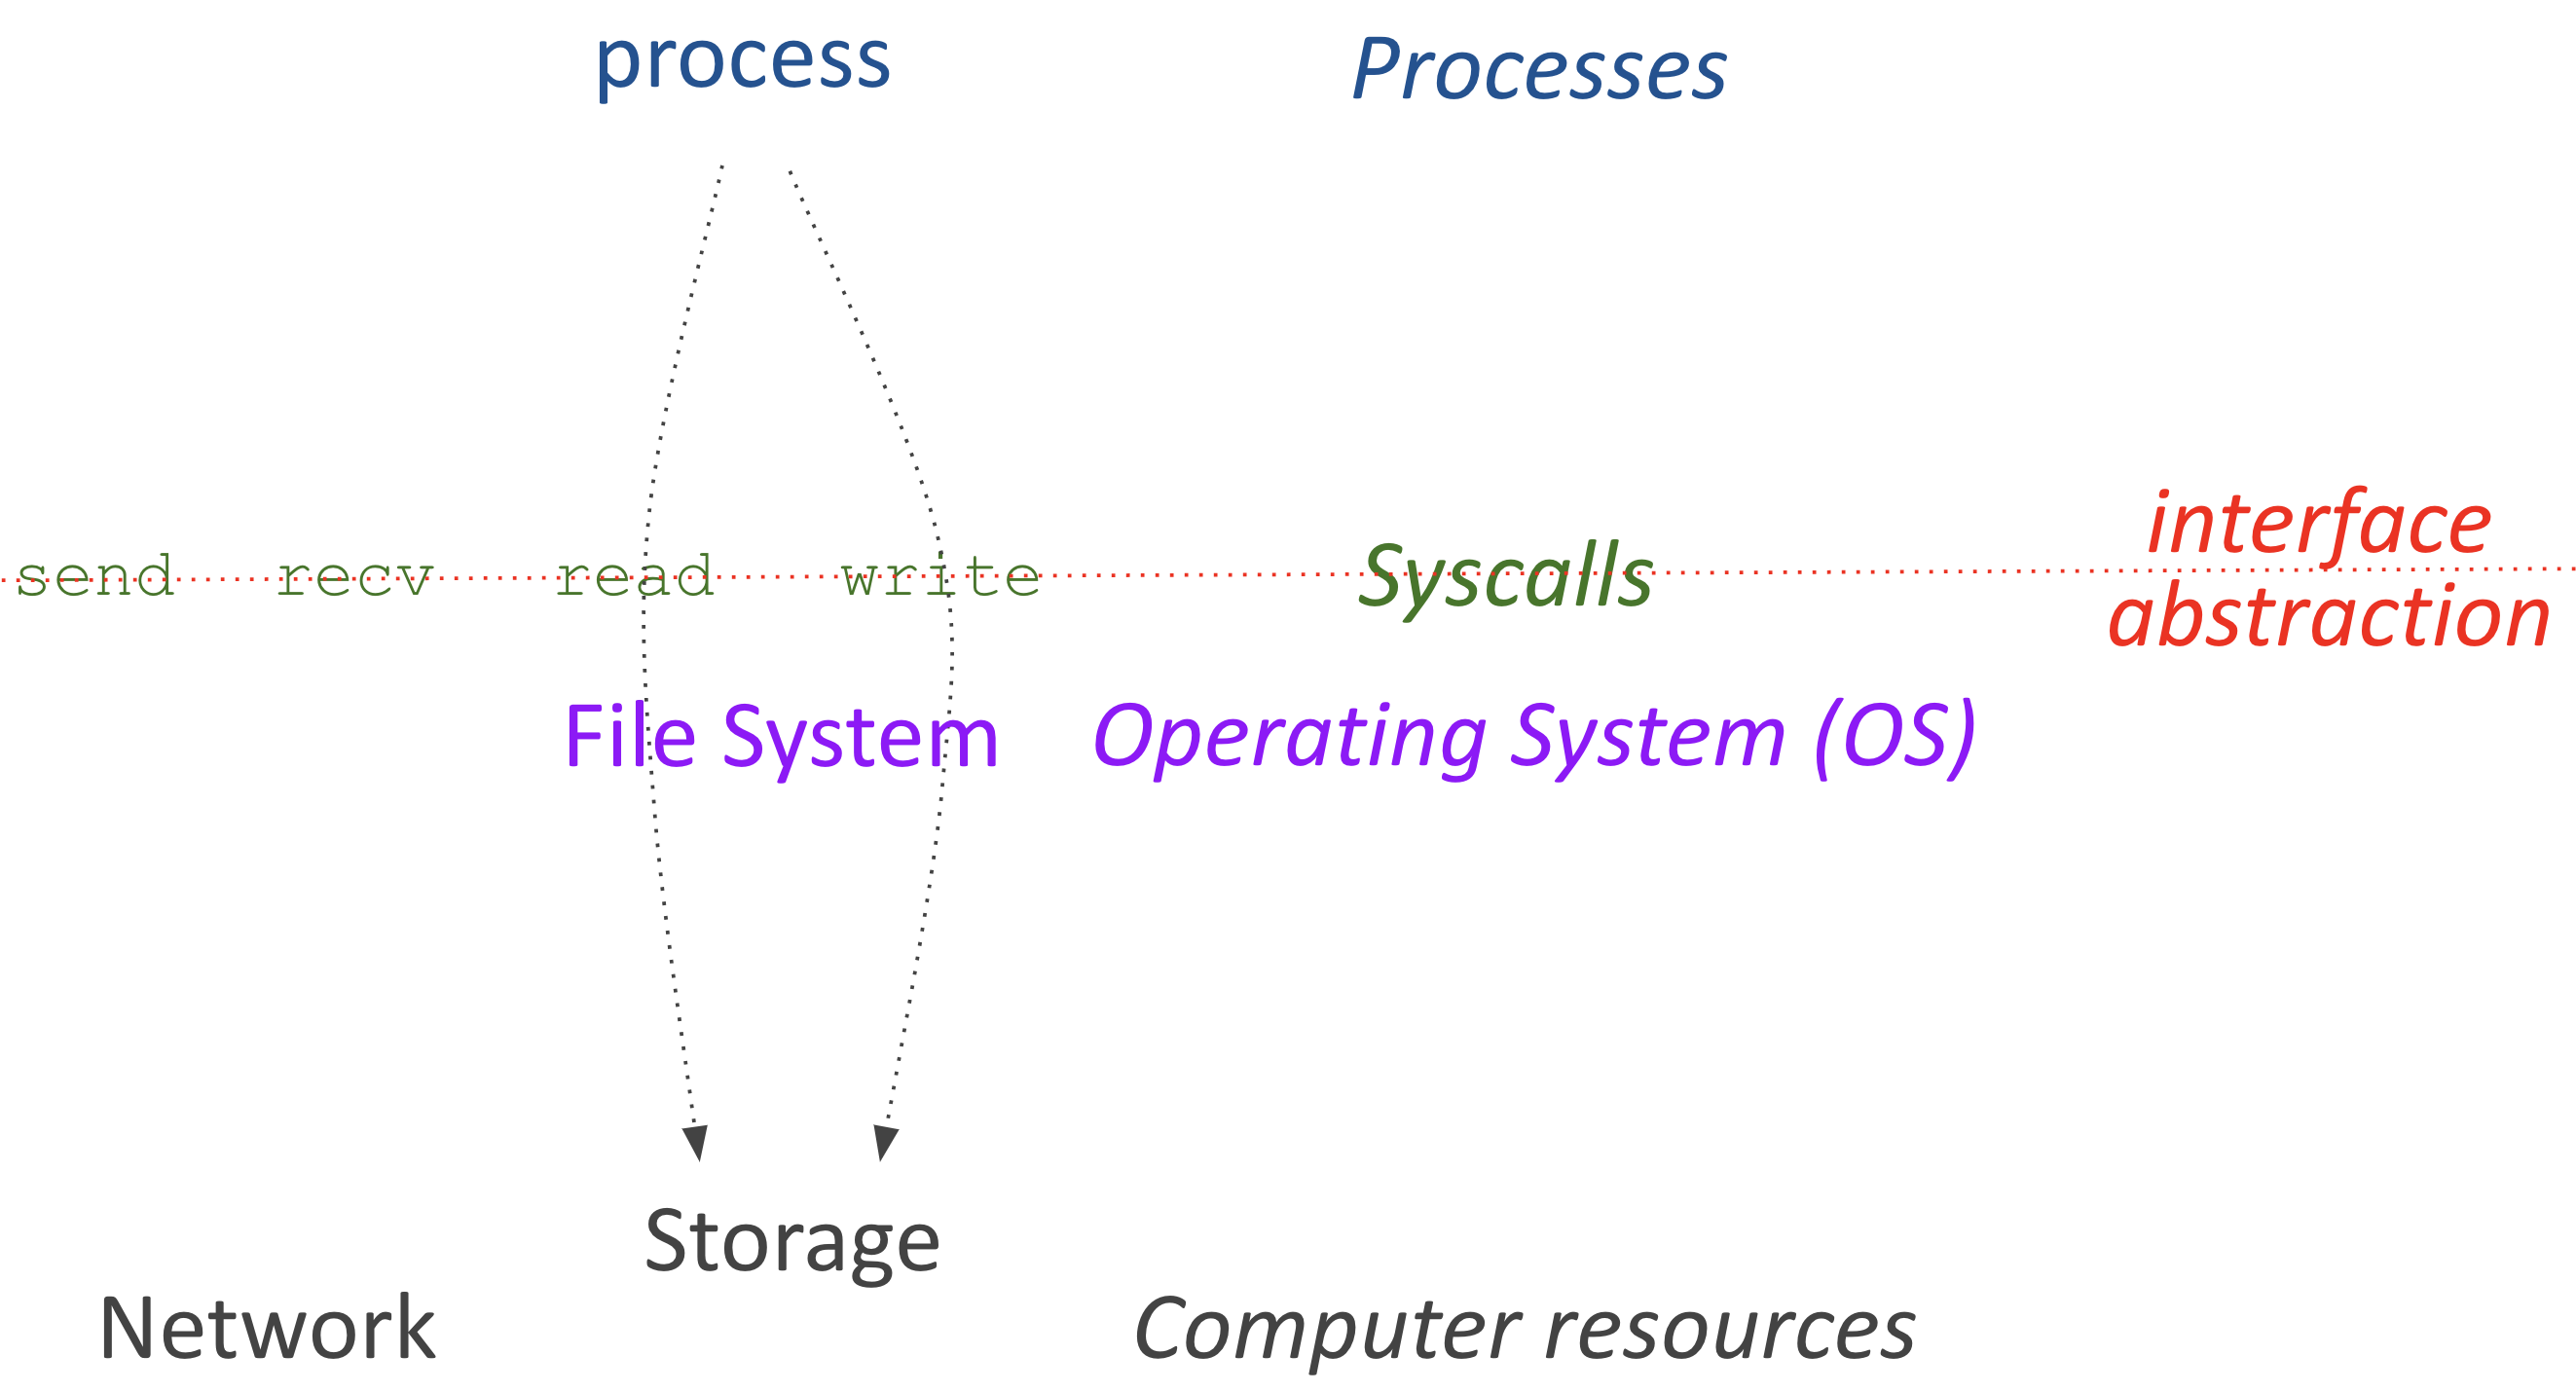
\includegraphics[width=0.65\textwidth]{chapters/L1/images/mix_int.png}
\end{center}
\vfill
\begin{definition}[Memory Access and I/O]
\textbf{Memory Access} refers to the CPU’s direct read/write operations using load/store instructions in main memory. In contrast, \textbf{I/O (Input/Output)} involves accessing external devices (such as storage or network) via system calls. I/O operations are generally more expensive because they require the CPU to switch context to execute privileged OS code.
\end{definition}
\vspace{0.5em}
\textbf{Exam Question:} How is reading from main memory different from reading from storage or the network? \\[0.5em]
\textbf{Answer:} Reading from main memory uses direct CPU instructions (load/store) and is very fast (tens to hundreds of nanoseconds), whereas reading from storage or the network requires a syscall, which interrupts the process and involves additional overhead (microseconds to milliseconds).
\vfill
\begin{definition}[I/O]
\textbf{I/O} (Input/Output) refers to operations that allow a process to access resources outside of its immediate control, such as storage devices or the network, via system calls. I/O operations are generally slower than direct memory accesses.
\end{definition}
\vspace{0.5em}
\textbf{Exam Question:} If a program does not create or manipulate any data, will executing this program require reading anything from memory?\\[0.5em]
\textbf{Answer:} Yes, executing the program will still require reading something from memory. Even if the program does not create or manipulate any data, the CPU must at least fetch the instructions of the program itself from memory

\newpage
%%%%%%%%%%%%%%%%%%%%%%%%%%%%%%%%%%%%%%%%%%%%%%%%%%%%%%%%%%%%%%%%%%%%%%
\vfill
\section{Communication Over the Internet}
Internet communication involves transferring data over a network where different latencies are encountered: \\
\begin{minipage}{0.45\textwidth}
  \begin{itemize}
    \item[-] Simple CPU instructions: \(\sim\)1~nsec.
    \item[-] Main memory accesses: tens to hundreds of nanoseconds.
    \item[-] Reading 1~KB from an SSD: tens to hundreds of microseconds.
    \item[-] Requesting data over the Internet: several to hundreds of milliseconds.
\end{itemize}
\end{minipage}
\hfill
\vline
\hfill
\begin{minipage}{0.45\textwidth}
\begin{center}
  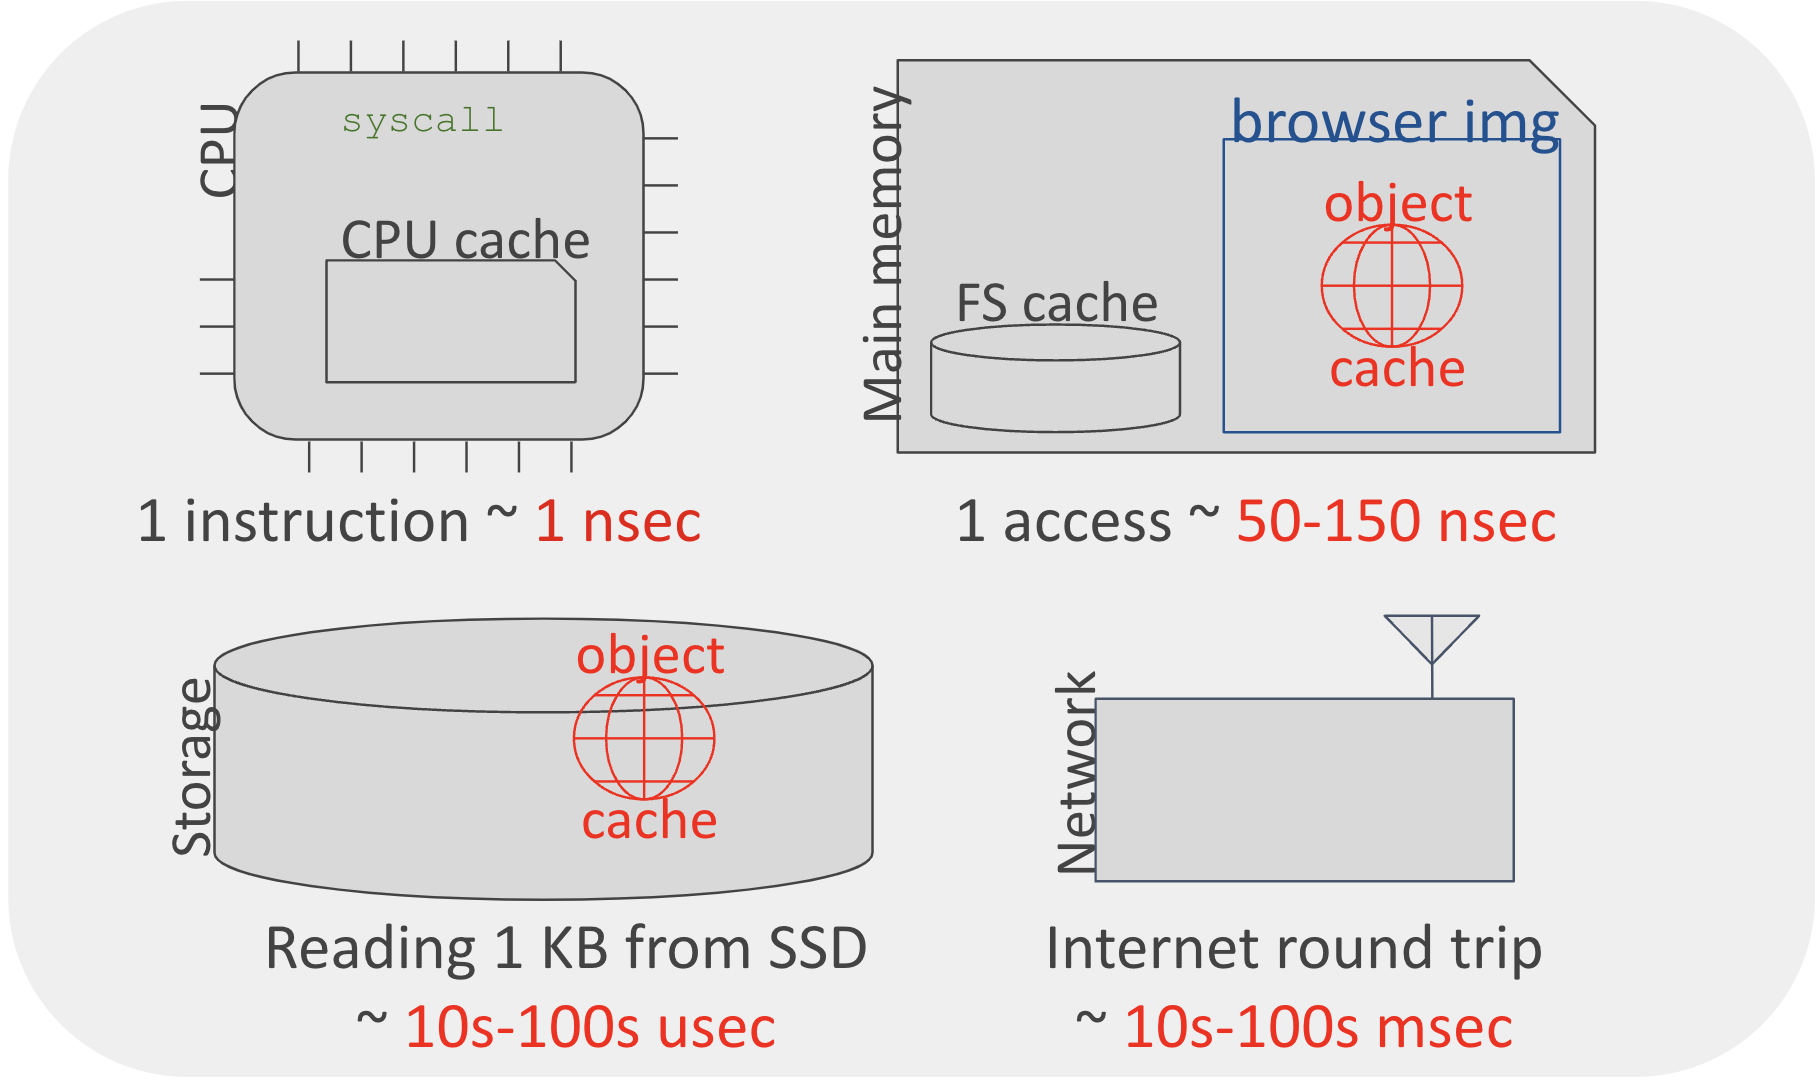
\includegraphics[width=1.15\textwidth]{chapters/L1/images/internet.png}
\end{center}
\end{minipage}\\[5px]
These delays make network communication expensive in terms of time, which is why caching is critical.
\vfill
%%%%%%%%%%%%%%%%%%%%%%%%%%%%%%%%%%%%%%%%%%%%%%%%%%%%%%%%%%%%%%%%%%%%%%
\subsection{End Systems}

The Internet is composed of \textbf{end systems}—devices that use the network for communication. These include laptops, smartphones, household appliances, connected cars, and even medical devices, as well as large cloud servers.

\begin{center}
  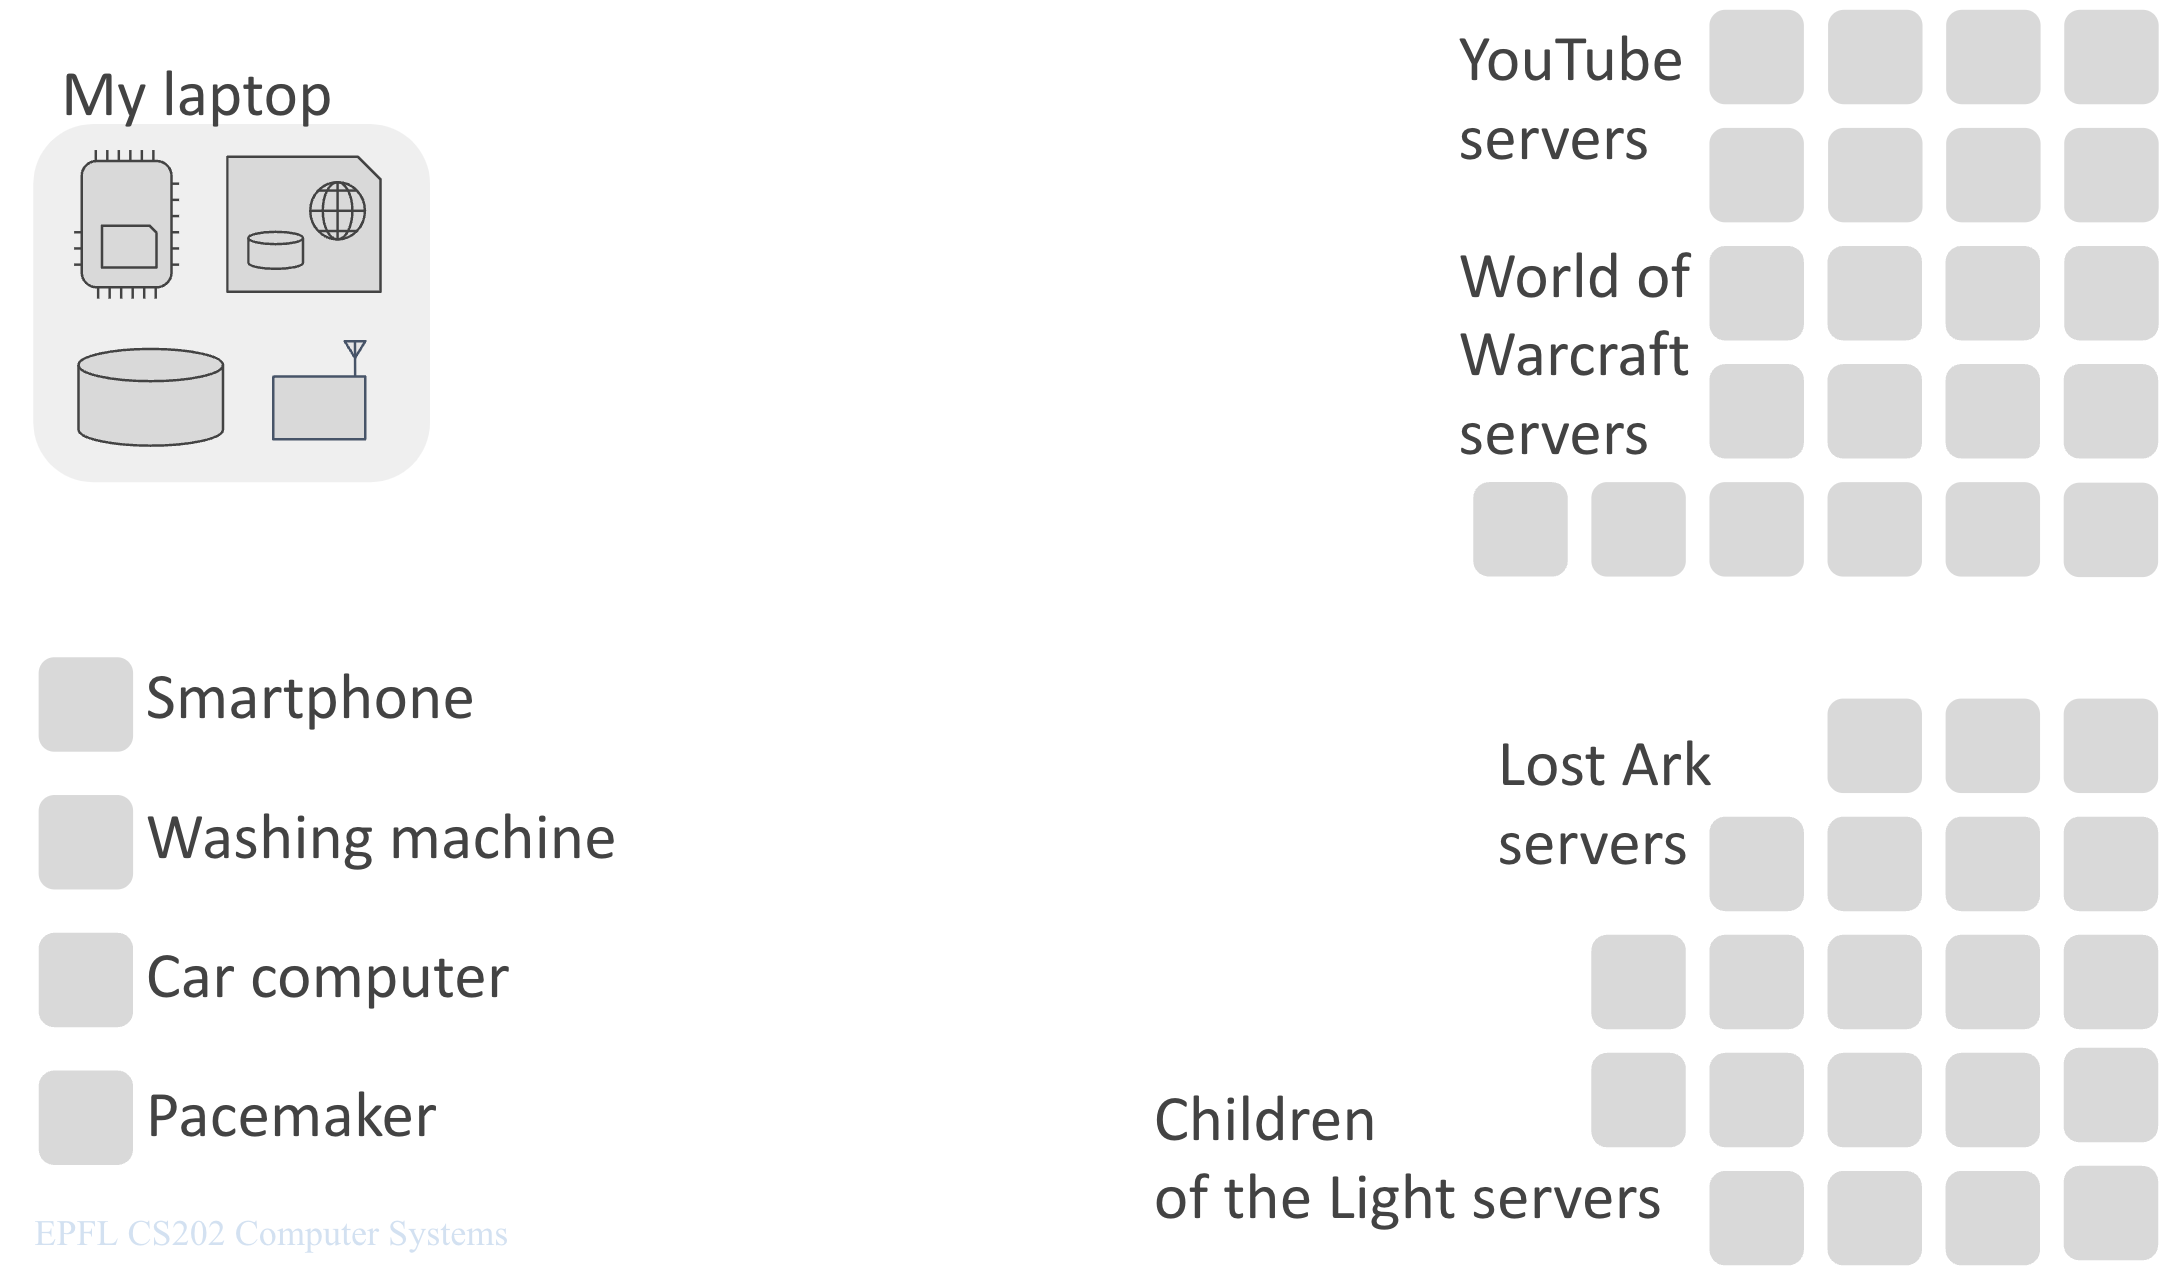
\includegraphics[width=0.65\textwidth]{chapters/L1/images/endsys.png}
\end{center}
\vfill
\newpage
%%%%%%%%%%%%%%%%%%%%%%%%%%%%%%%%%%%%%%%%%%%%%%%%%%%%%%%%%%%%%%%%%%%%%%
\subsection{Packet Switches and Network Links}

In addition to end systems, the Internet relies on:
\begin{itemize}
  \item[-] \textbf{Packet Switches}: Devices that route data between end systems.
  \item[-] \textbf{Network Links}: Physical connections that interconnect packet switches and end systems.
\end{itemize}

These components are managed by Internet Service Providers (ISPs) as well as major cloud providers.

\begin{center}
  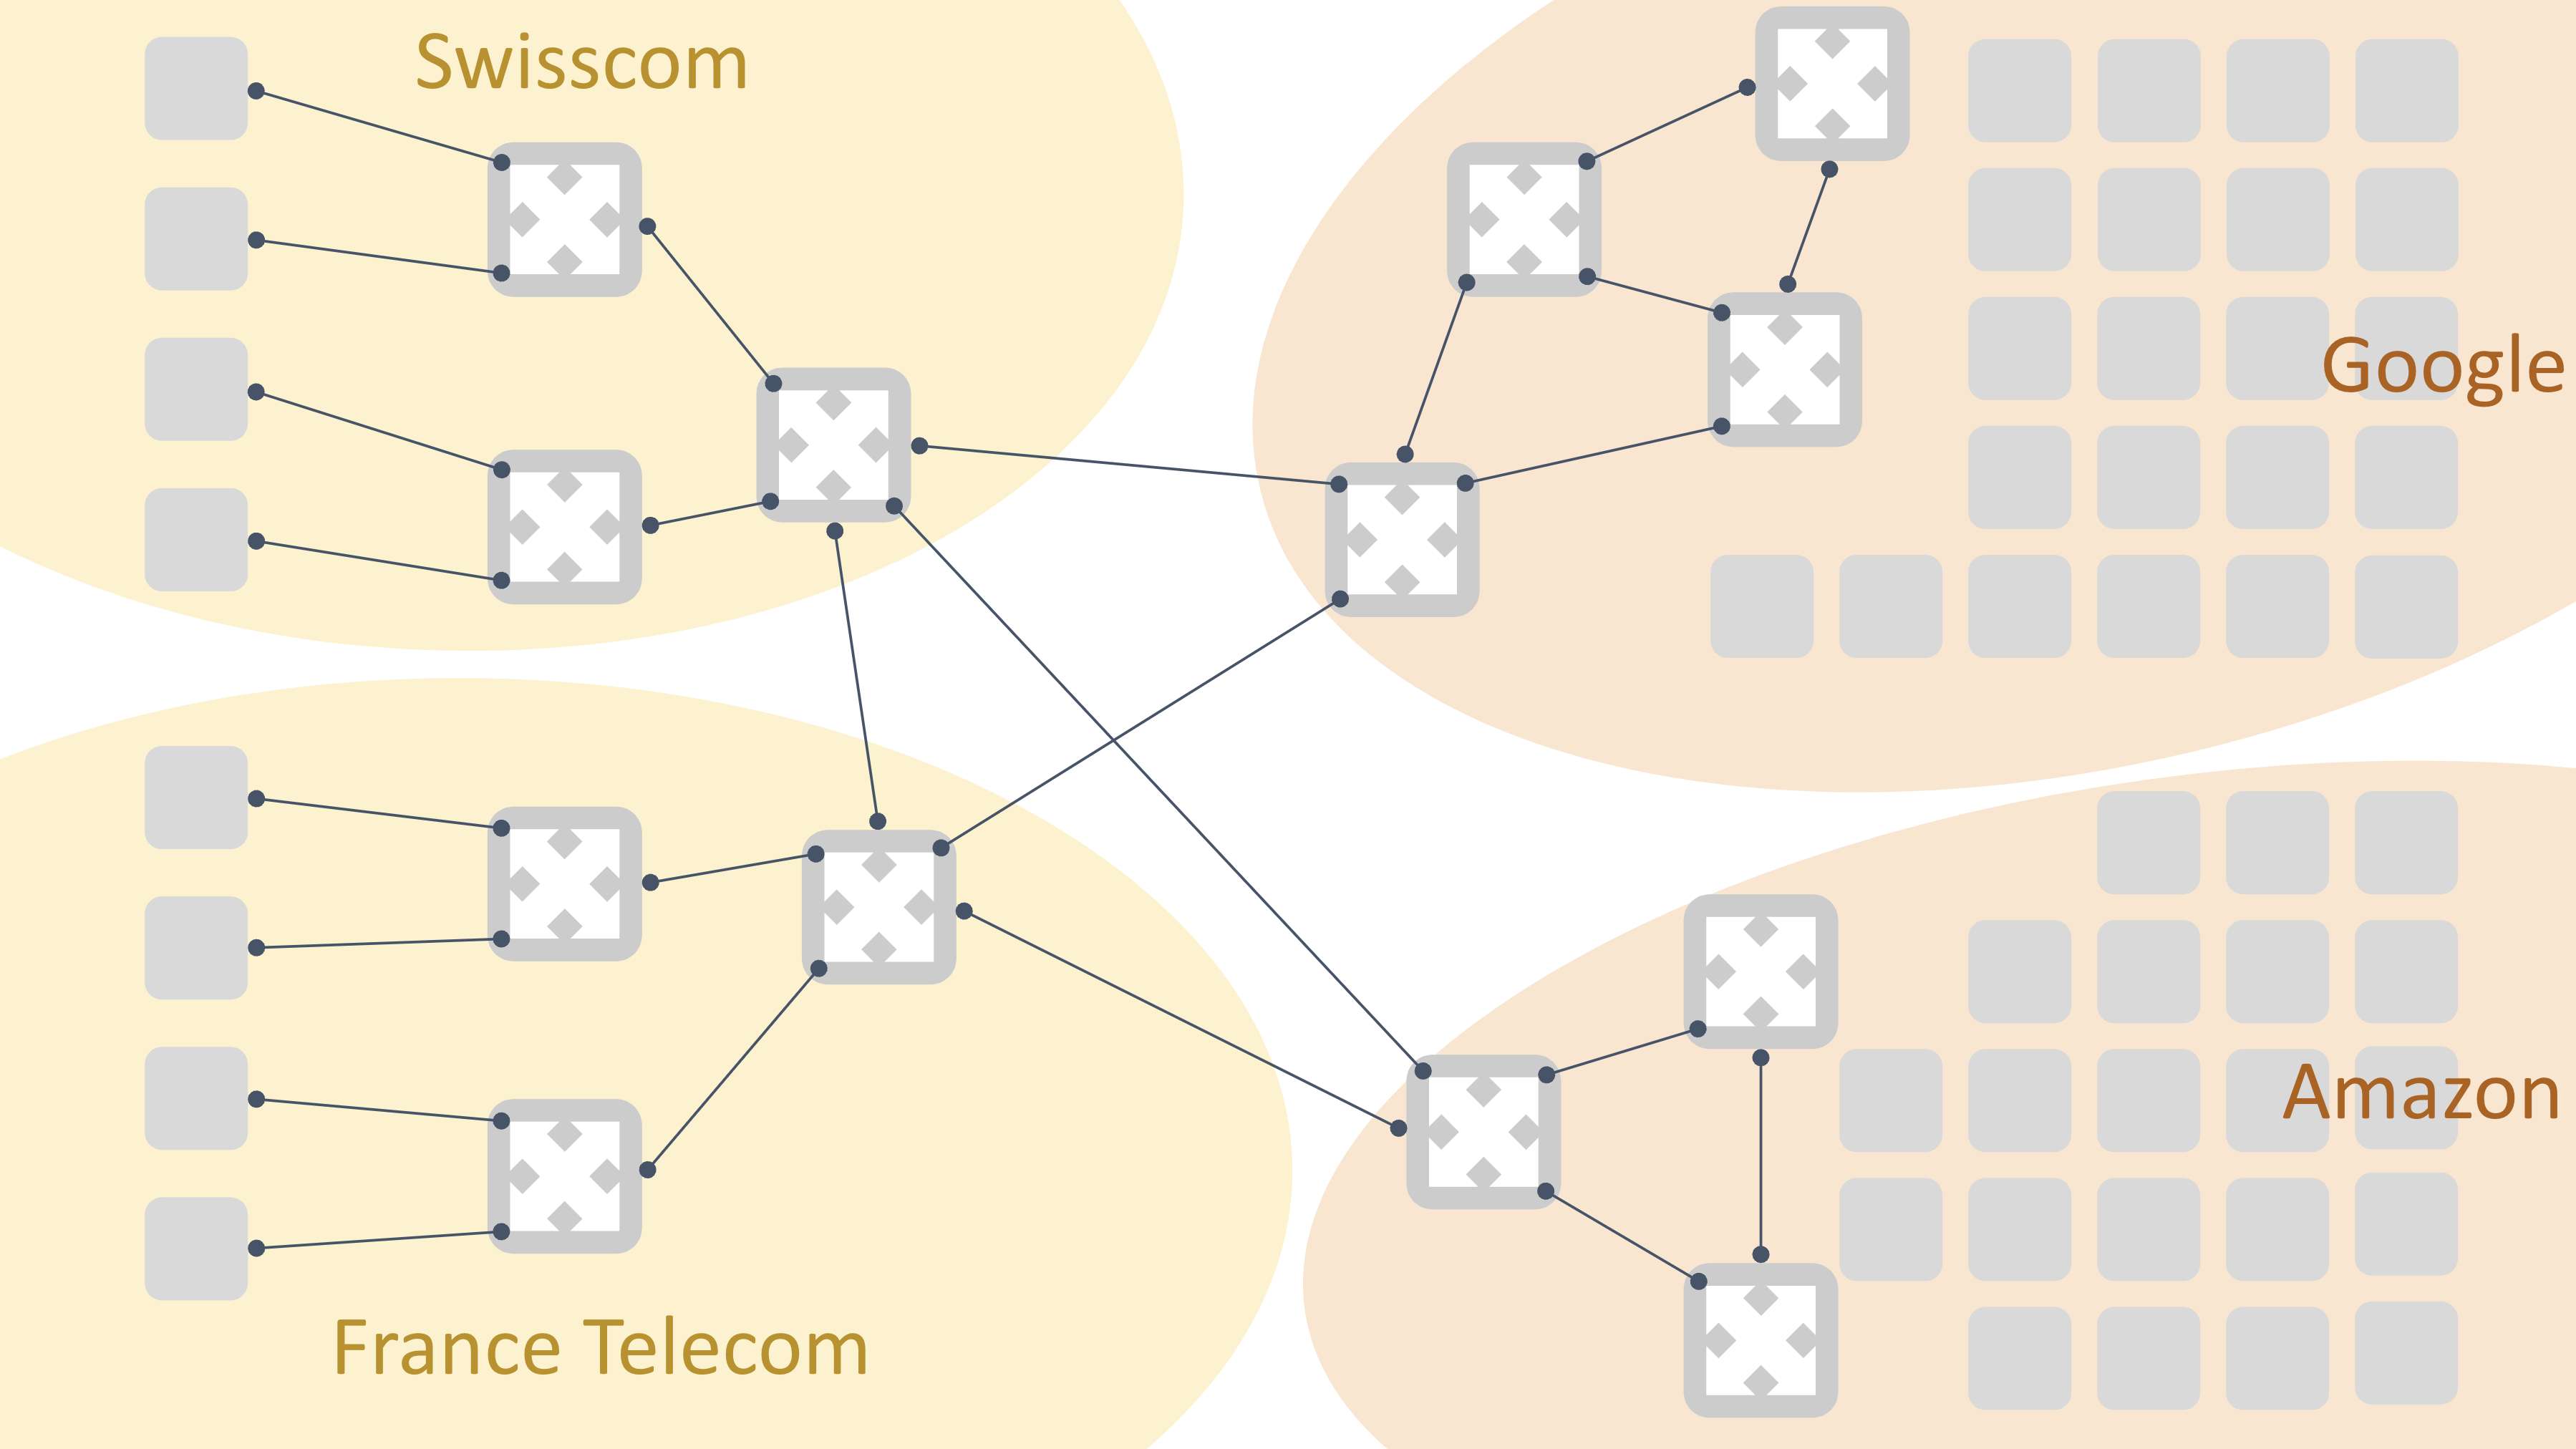
\includegraphics[width=0.65\textwidth]{chapters/L1/images/internet_schema.png}
\end{center}

%%%%%%%%%%%%%%%%%%%%%%%%%%%%%%%%%%%%%%%%%%%%%%%%%%%%%%%%%%%%%%%%%%%%%%
\subsection{Edge Caches}
To reduce the load on cloud data centers and improve user performance, large cloud providers often deploy \textbf{edge caches} within ISP networks. These caches store frequently accessed content closer to the end-users, reducing latency and network traffic.
\begin{center}
  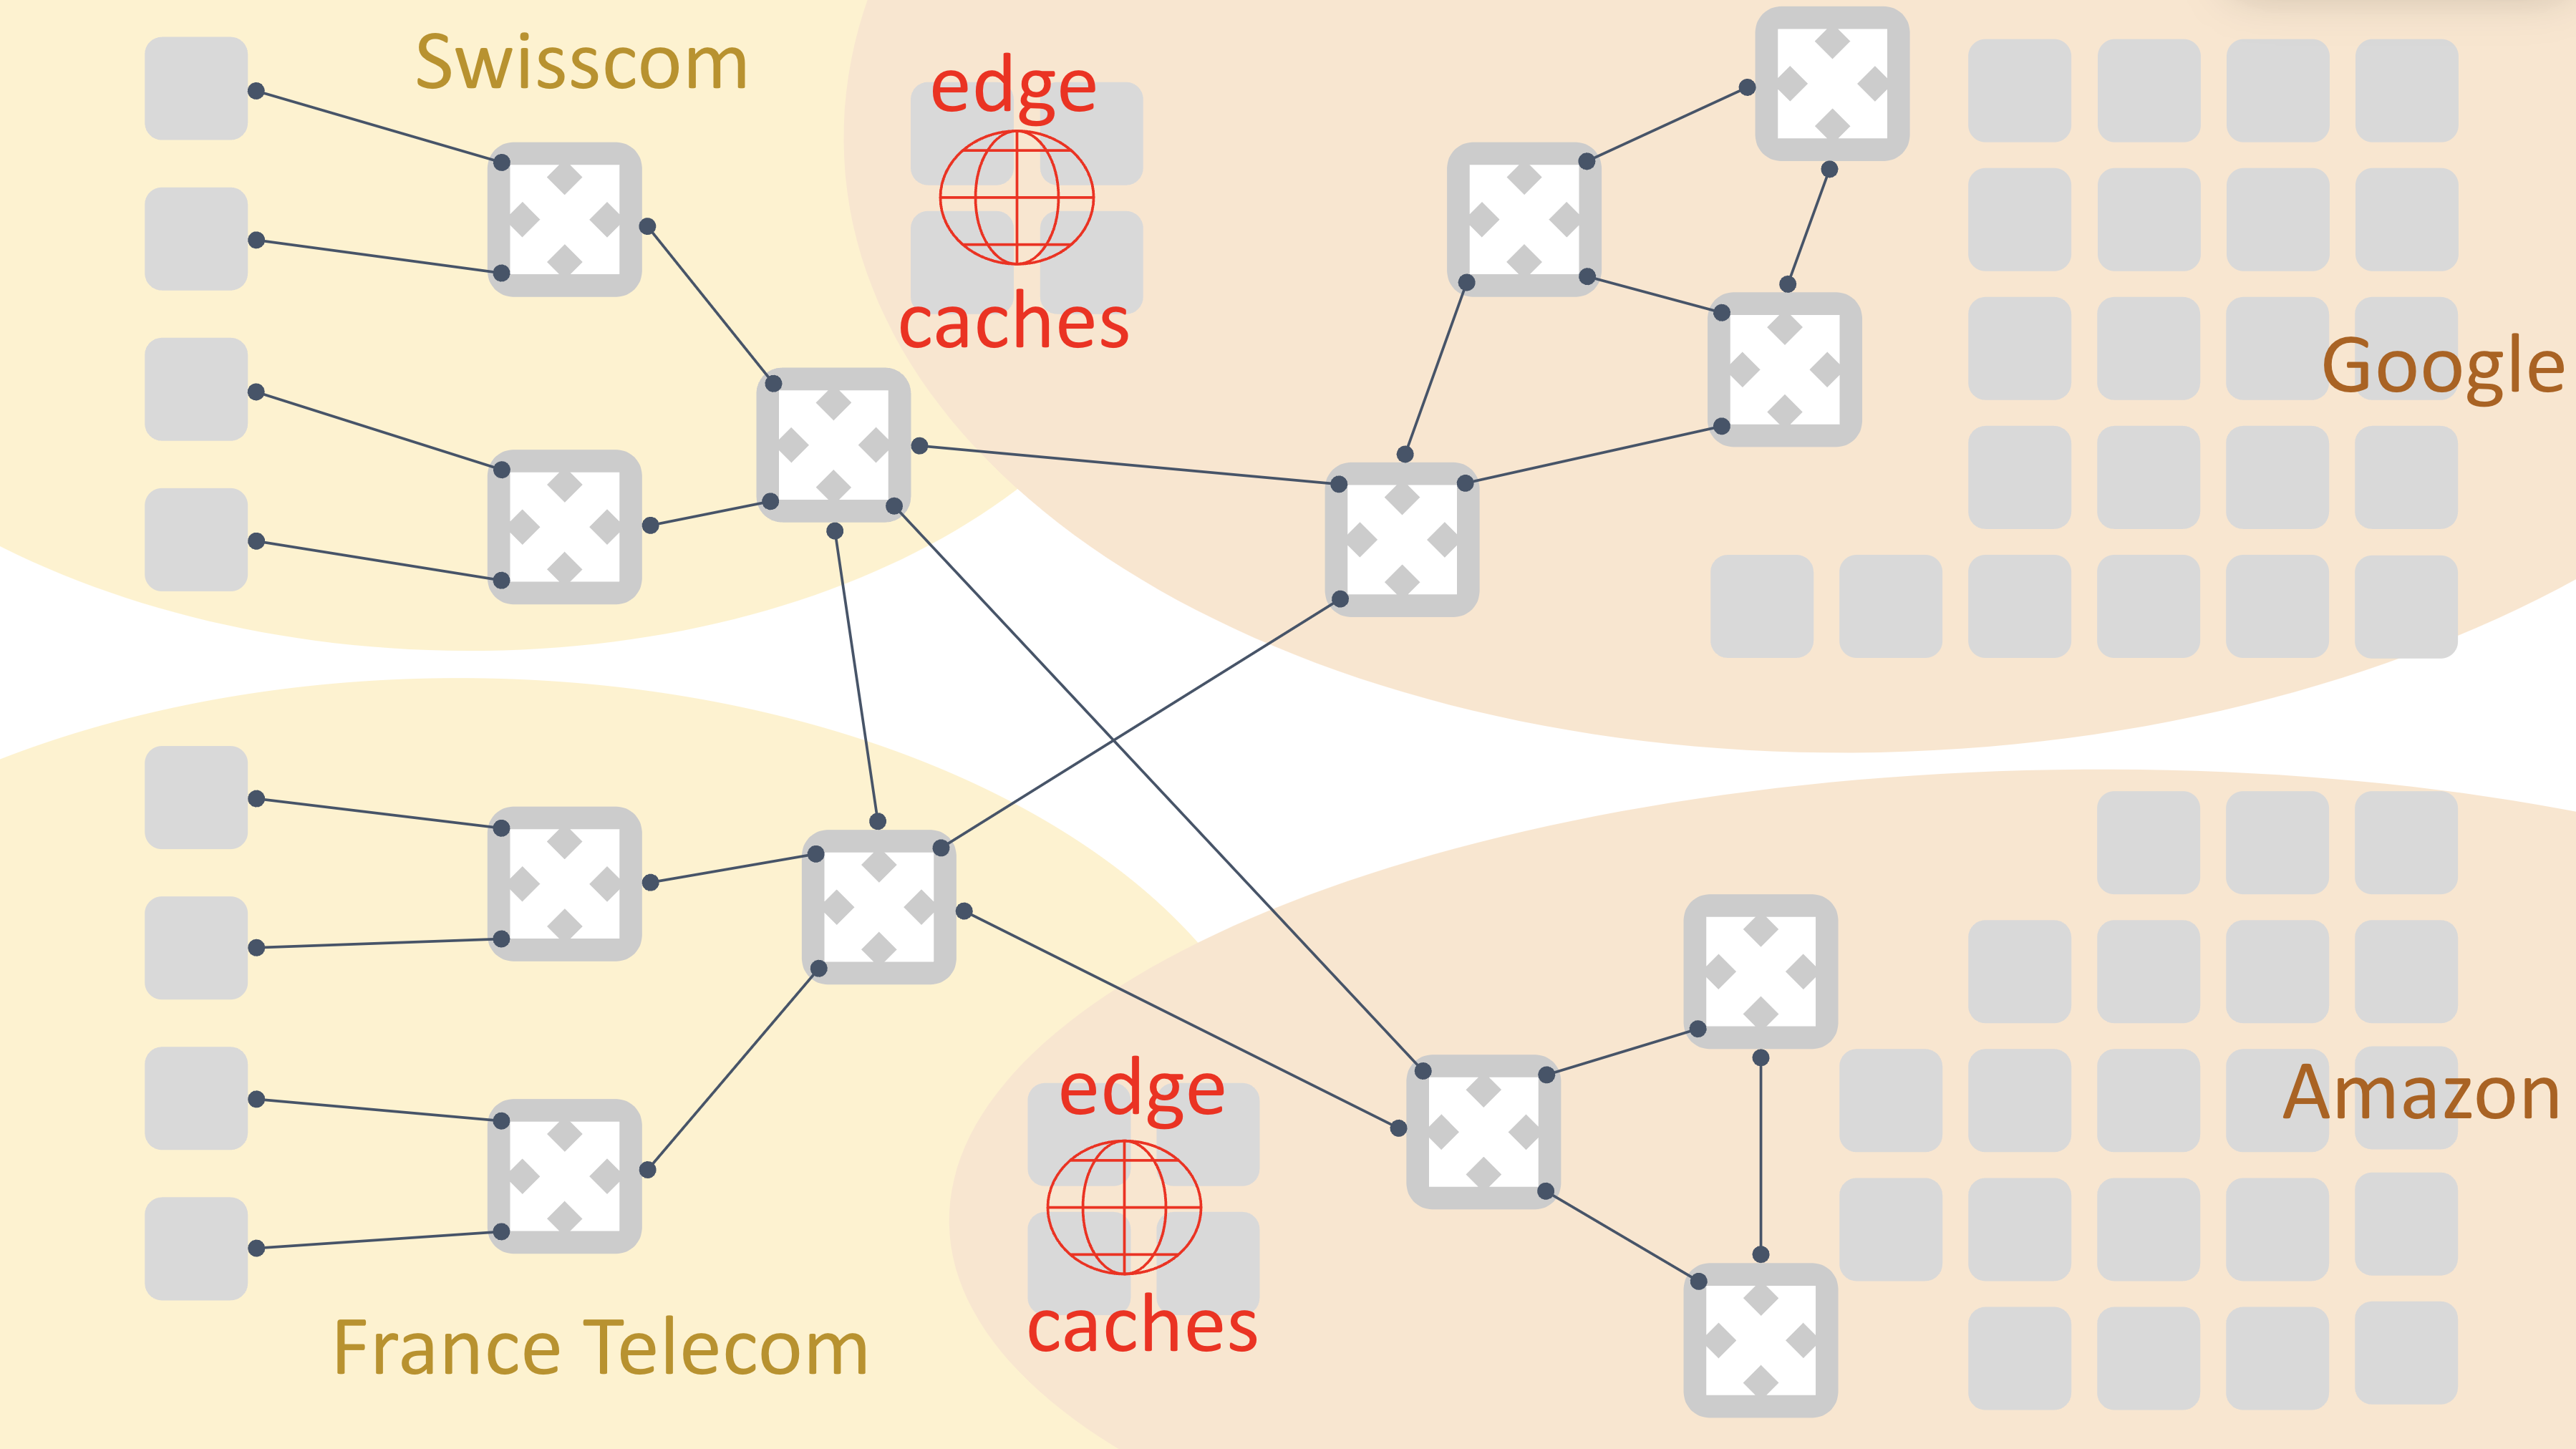
\includegraphics[width=0.65\textwidth]{chapters/L1/images/edge_caches.png}
\end{center}
%%%%%%%%%%%%%%%%%%%%%%%%%%%%%%%%%%%%%%%%%%%%%%%%%%%%%%%%%%%%%%%%%%%%%%
\section{Summary}
In this lecture, we traced the journey of a YouTube video and introduced several fundamental concepts:
\begin{itemize}
  \item \textbf{Programs, Processes, and Threads:} Programs stored on disk become processes (and threads) when executed.
  \item \textbf{Distributed Applications:} Different processes communicate over networks using well-defined communication protocols.
  \item \textbf{Interfaces and Abstractions:} System calls, APIs, and caching abstract the complexity of hardware resources.
  \item \textbf{The Operating System:} Acts as an intermediary between processes and hardware resources.
  \item \textbf{Performance Considerations:} Frequency imbalances between the CPU and memory are mitigated by caching at various levels (CPU cache, file system cache, object caches).
\end{itemize}

\begin{center}
  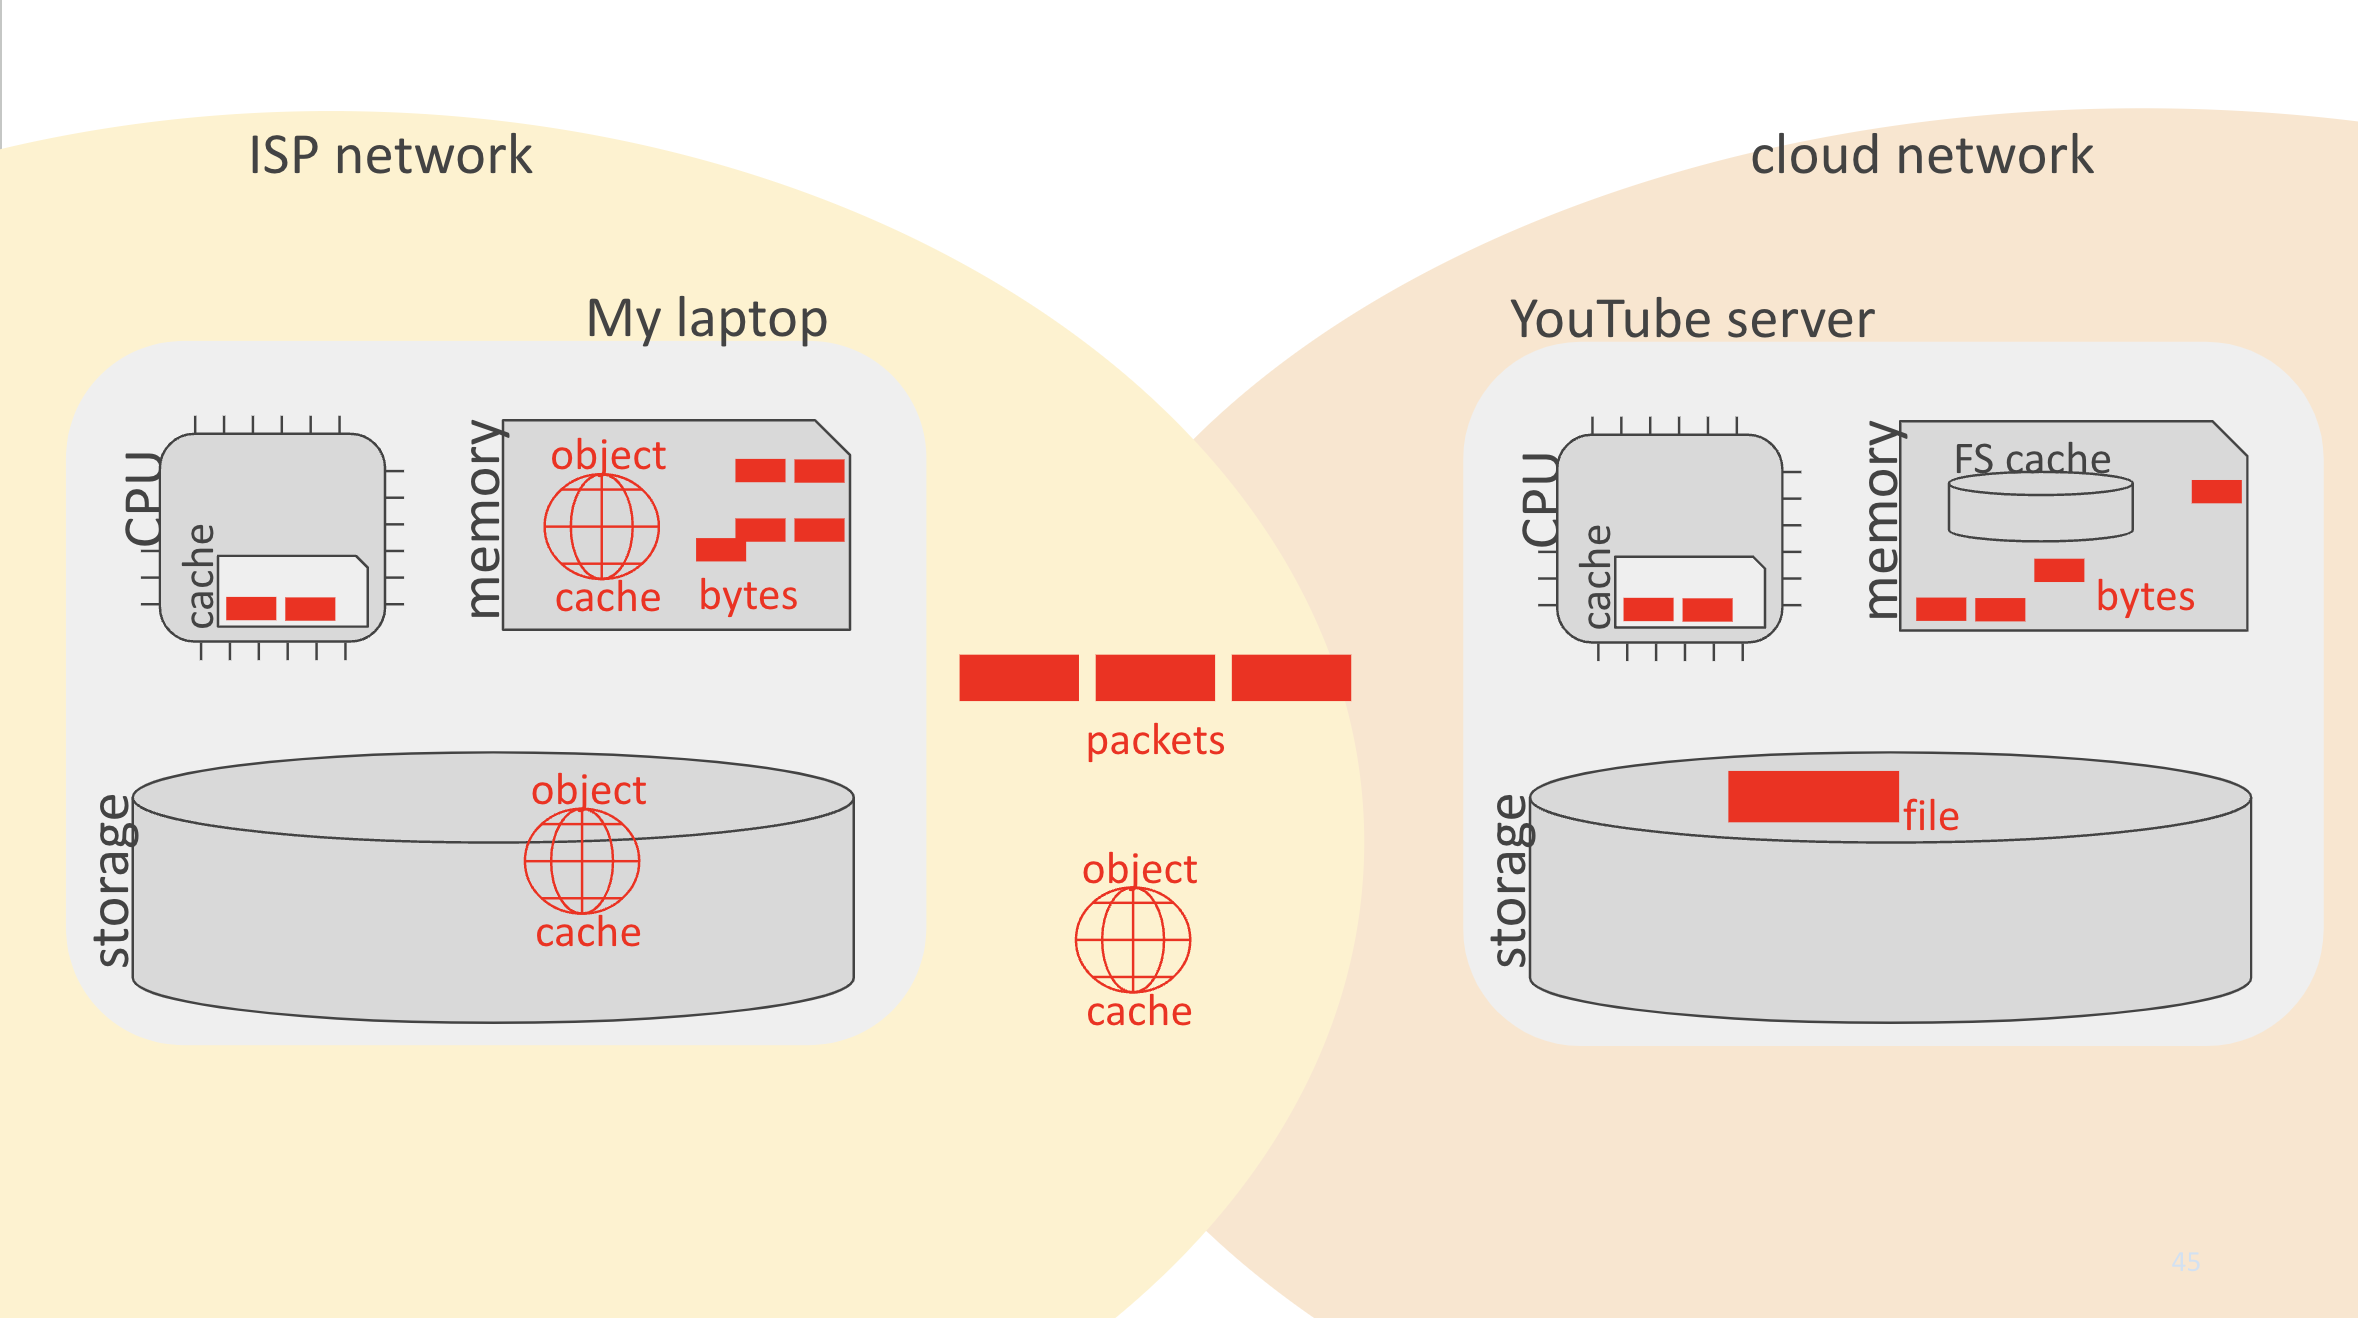
\includegraphics[width=0.65\textwidth]{chapters/L1/images/conclusion_youtube.png}
\end{center}

 

\chapter{L2 - All About Processes}
This chapter provides an overview of the fundamental concepts underlying modern process management and memory organization in computer systems. We discuss multithreading, CPU registers, the role of compilers, and memory organization—including both stack and heap memory—as well as virtualization techniques that allow multiple processes to coexist seamlessly.
\small
\section{Multithreading}
When a program runs, the processor loads it into main memory and creates a thread. In a multithreaded program, there is typically one \emph{manager} thread that delegates work to several \emph{worker} threads. For instance, when computing the sum of a large set of numbers, the workload can be divided into subsets, with each worker thread processing a portion of the data while the manager coordinates the overall computation.

\begin{center}
    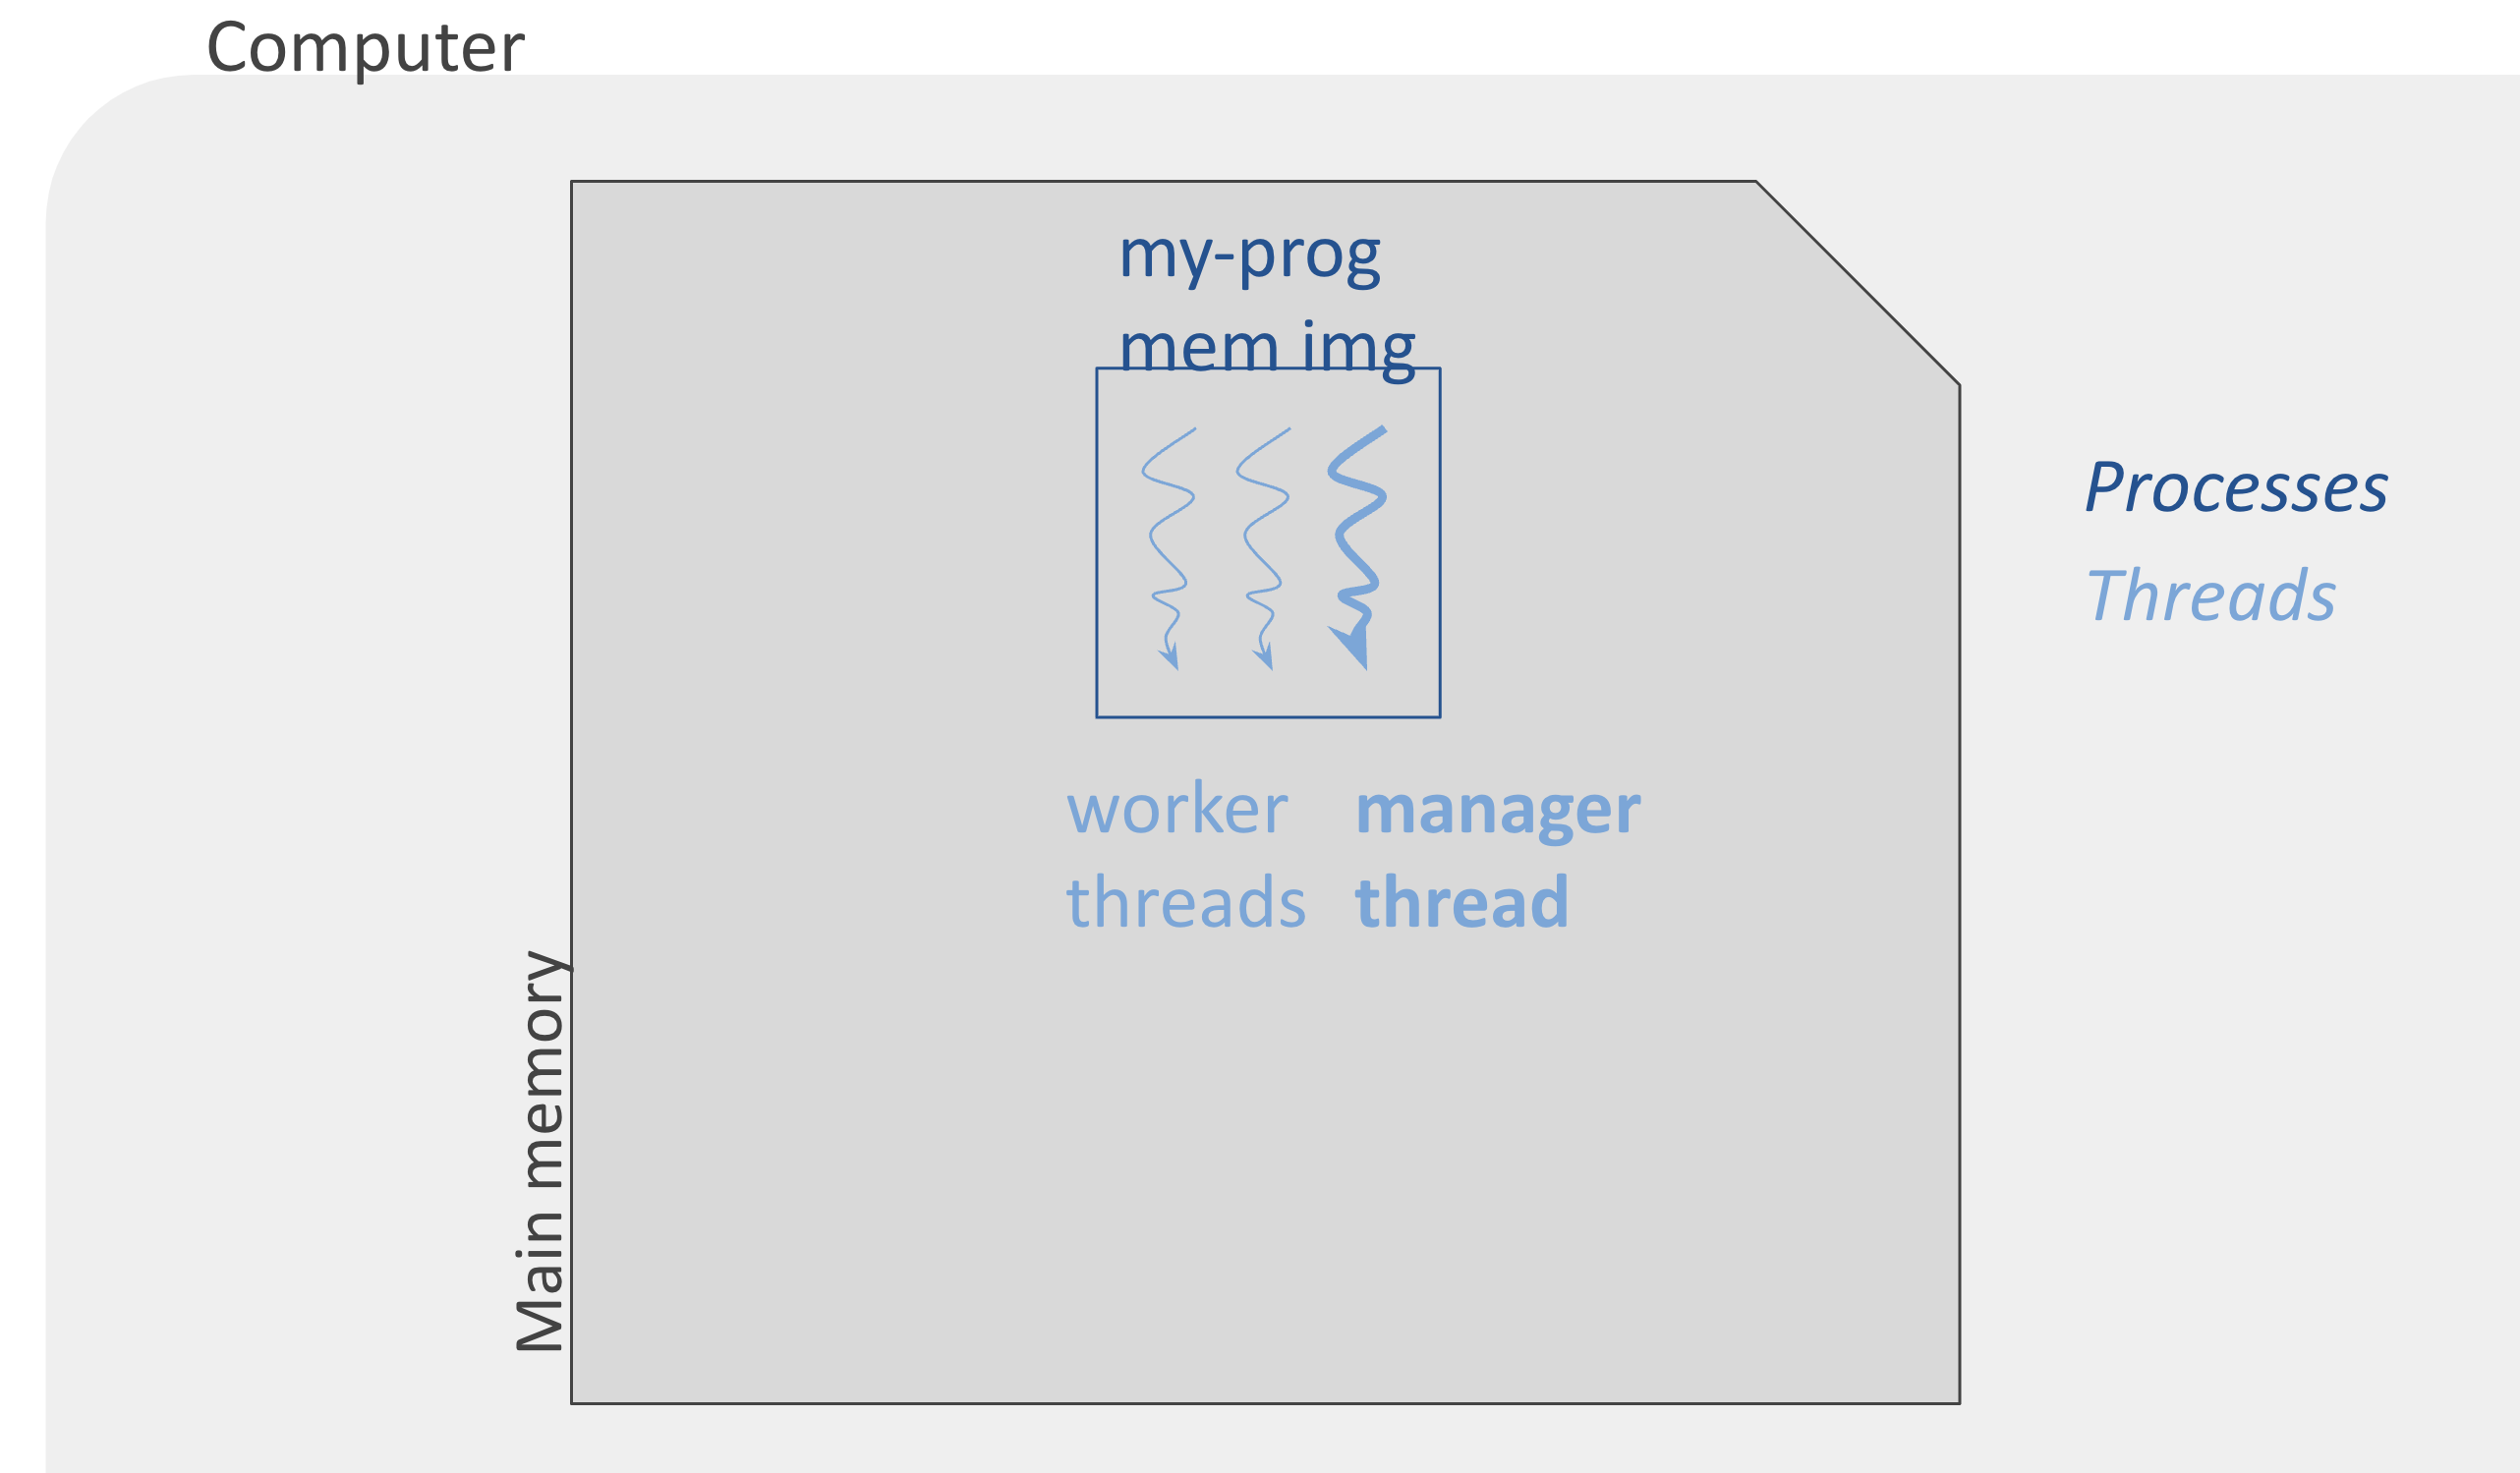
\includegraphics[width=0.55\textwidth]{chapters/L2/images/multi_threads.png}
\end{center}

\section{Registers}
\begin{minipage}{0.45\textwidth}
CPU registers are small storage locations within the processor that hold data and instructions needed during execution. For example, the \texttt{mov} instruction might transfer data from one register (or memory location) to another. Key registers include:
\begin{itemize}
  \item[-] \textbf{Instruction Pointer (IP):} Keeps track of the next instruction to be executed.
  \item[-] \textbf{Stack Pointer (SP):} Points to the current top of the stack in main memory.
\end{itemize}
\end{minipage}
\hfill
\vline
\hfill
\begin{minipage}{0.45\textwidth} 
\begin{center}
    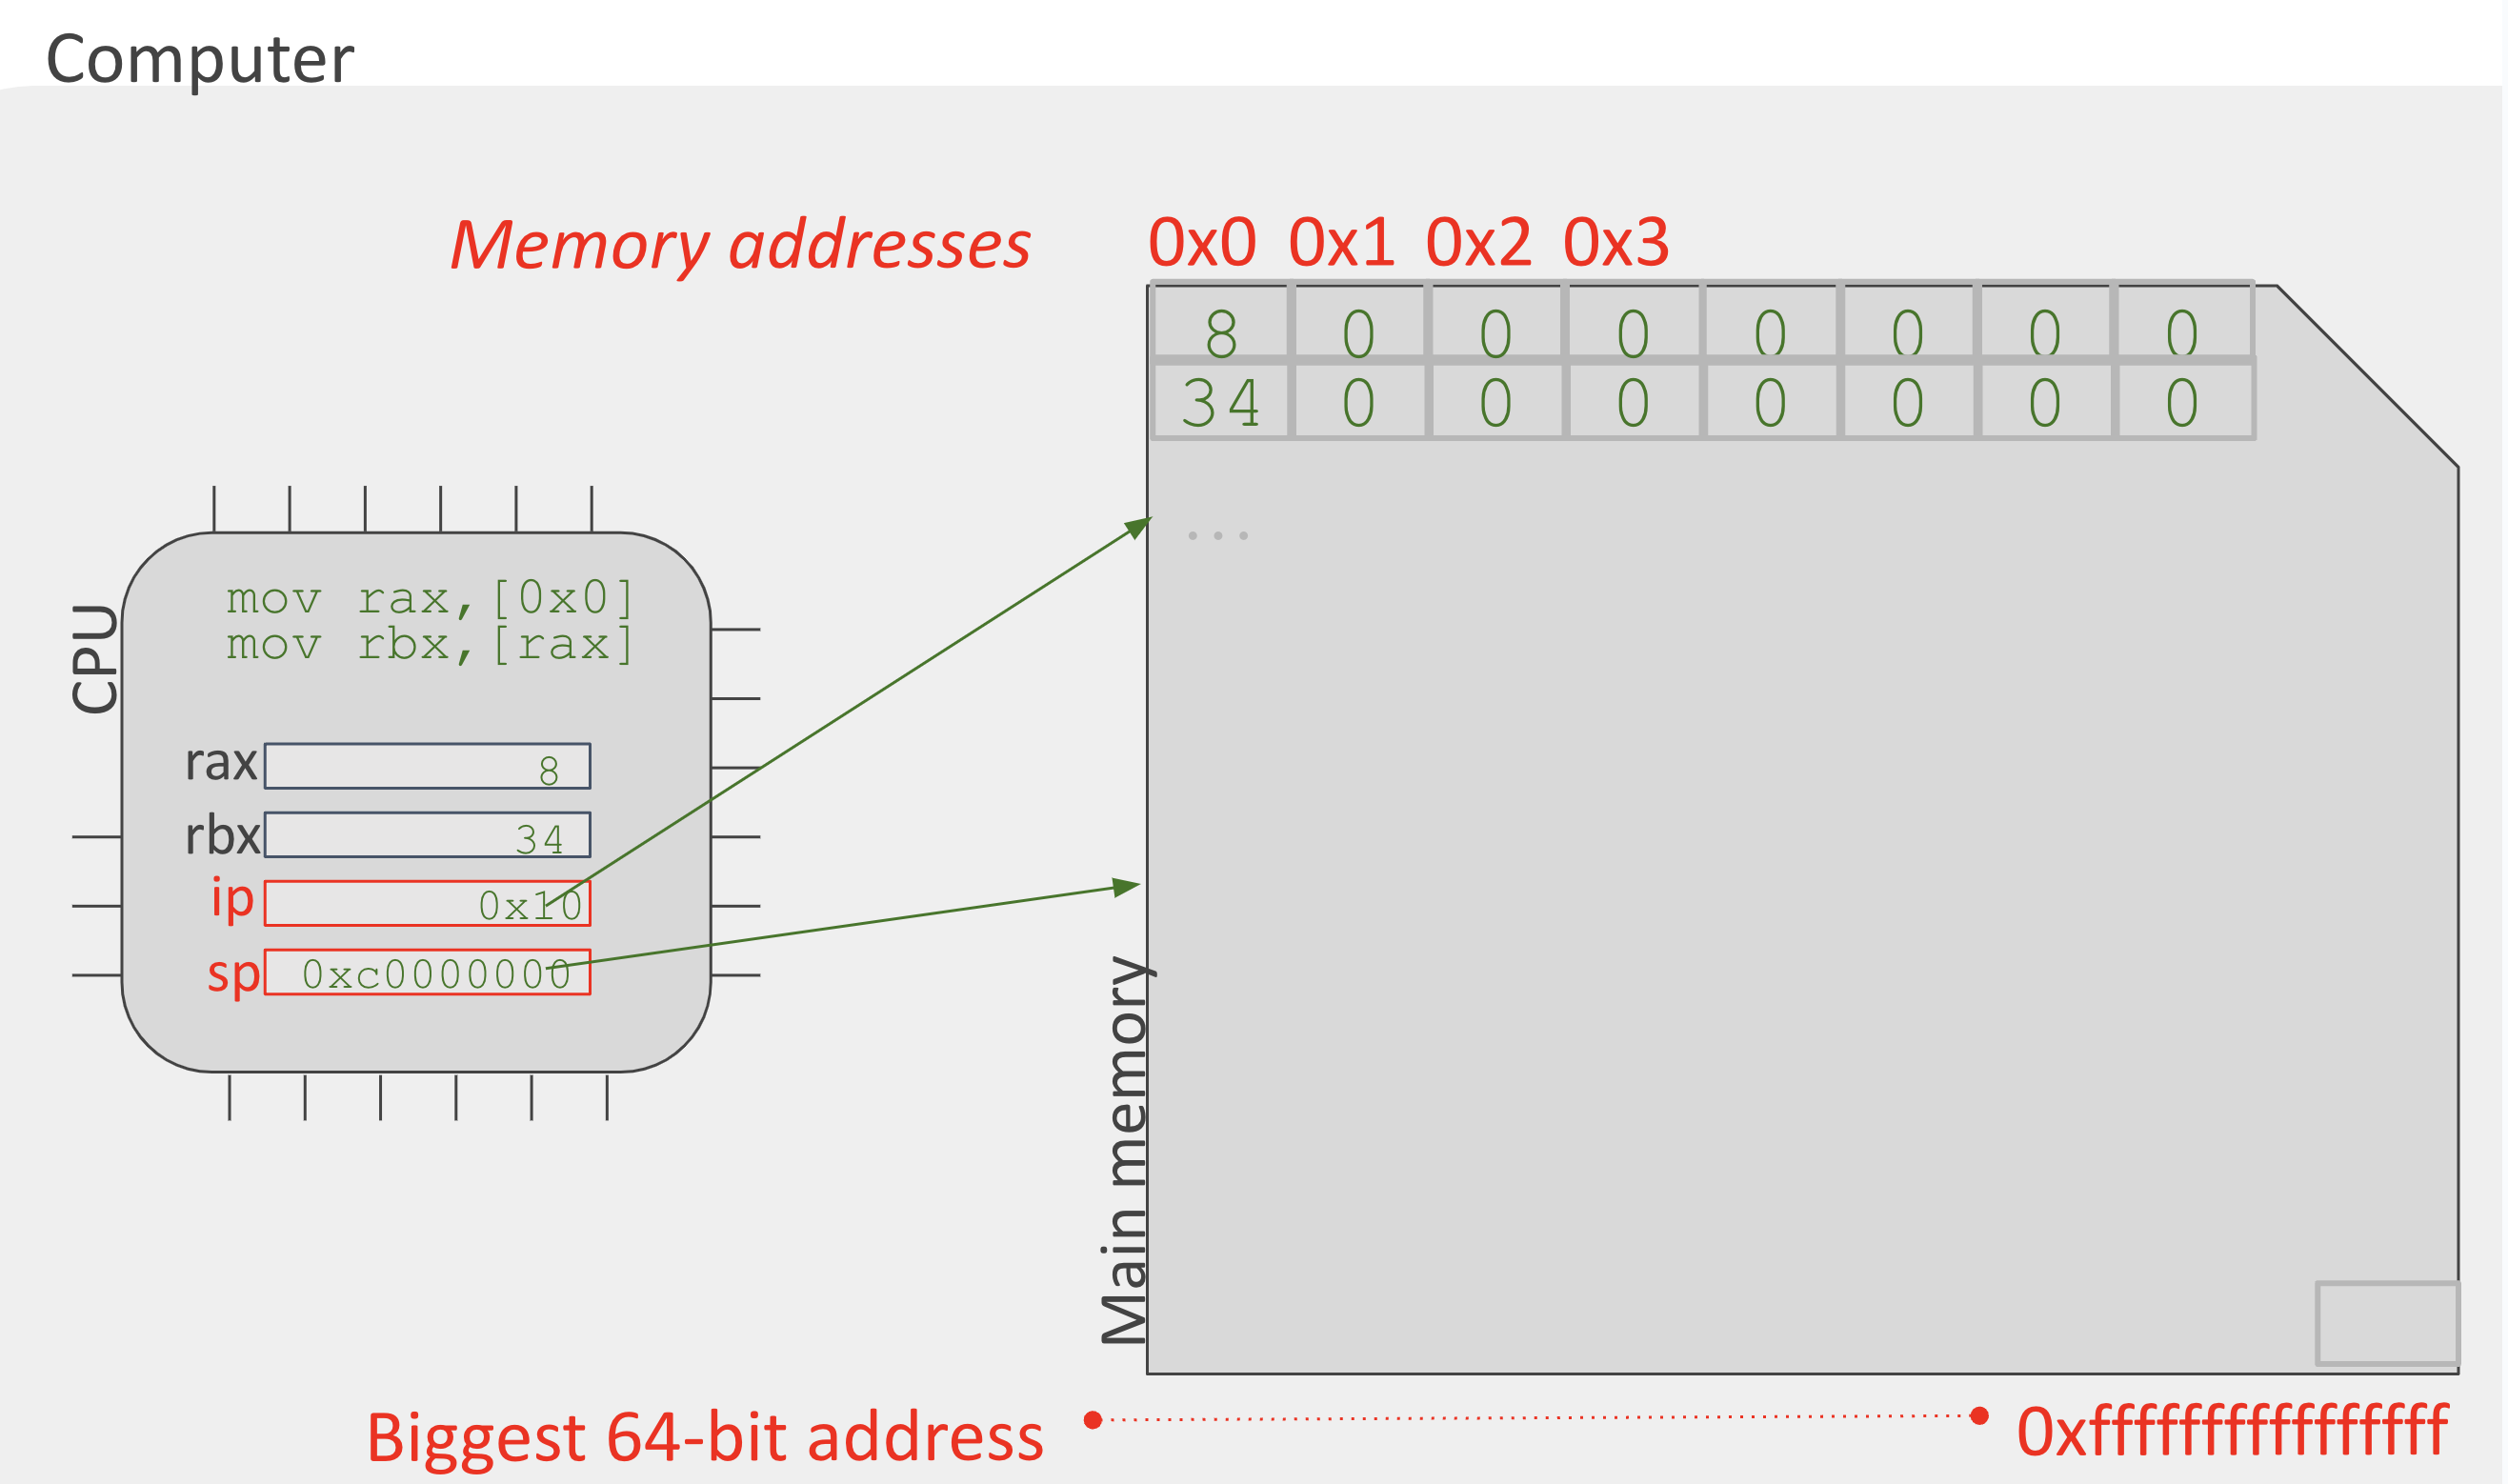
\includegraphics[width=1.1\textwidth]{chapters/L2/images/registers.png}
\end{center}
\end{minipage}
\newpage
\begin{definition}[Compiler]
A compiler translates high-level source code (such as C) into low-level executable code (often Assembly language). This translation involves parsing, optimization, and the generation of machine-specific instructions.
\end{definition}

\section{Memory Organization}
\textit{I'll go a little bit deeper for our fellow syscoms, I also recommend understanding how LIFO works before reading this, if you're too lazy for that, it's basically in the name Last In First Out, means that the last item pushed onto the stack is the first one to be removed, just like stacking plates— you take the top plate first before reaching the ones below. } \\
In modern computer architectures, a process's memory is divided into several distinct segments, each serving a specific role during program execution. Understanding these segments is fundamental for effective programming and debugging. \\[10px]

\begin{definition}[Memory Segments]
A process's memory image is typically divided into the following segments:
\begin{itemize}
    \item \textbf{Text Segment:} Contains the executable code and embedded constants. It is usually marked as read-only to prevent accidental modification.
    \item \textbf{Data Segment:} Stores global and static variables. This segment is often subdivided into:
        \begin{itemize}
            \item \textbf{Initialized Data:} Variables explicitly initialized by the programmer.
            \item \textbf{Uninitialized Data (BSS):} Variables that are declared but not explicitly initialized, and are set to zero by default.
        \end{itemize}
    \item \textbf{Heap Segment:} Used for dynamic memory allocation. Memory here is allocated and deallocated during runtime by the programmer (or automatically via garbage collection in some languages). The heap typically grows upward (from lower to higher memory addresses).
    \item \textbf{Stack:} Manages function calls, local variables, and function parameters. The stack is automatically managed by the CPU, growing downward (from higher to lower memory addresses) as functions are called.
\end{itemize}
\end{definition}

\subsection{The Stack}

The stack is a dedicated region of memory that the CPU uses to manage function calls and local variables. When a function is invoked:
\begin{enumerate}
    \item The CPU executes a \texttt{call} instruction, which pushes the return address onto the stack.
    \item A new \emph{stack frame} is created to store local variables and function-specific data.
    \item Upon function return, the stack frame is removed (or "unwound"), and control returns to the calling function.
\end{enumerate}

\begin{minipage}{0.45\textwidth}
\textbf{Key Characteristics of the Stack:}
\begin{itemize}
    \item \textbf{Automatic Management:} The CPU automatically handles pushing and popping of data.
    \item \textbf{Growth Direction:} Grows downward, from higher to lower memory addresses.
    \item \textbf{Contents:} Stores return addresses, local variables, and sometimes function arguments.
\end{itemize}
\end{minipage}
\hfill
\begin{minipage}{0.45\textwidth}
\begin{center}
    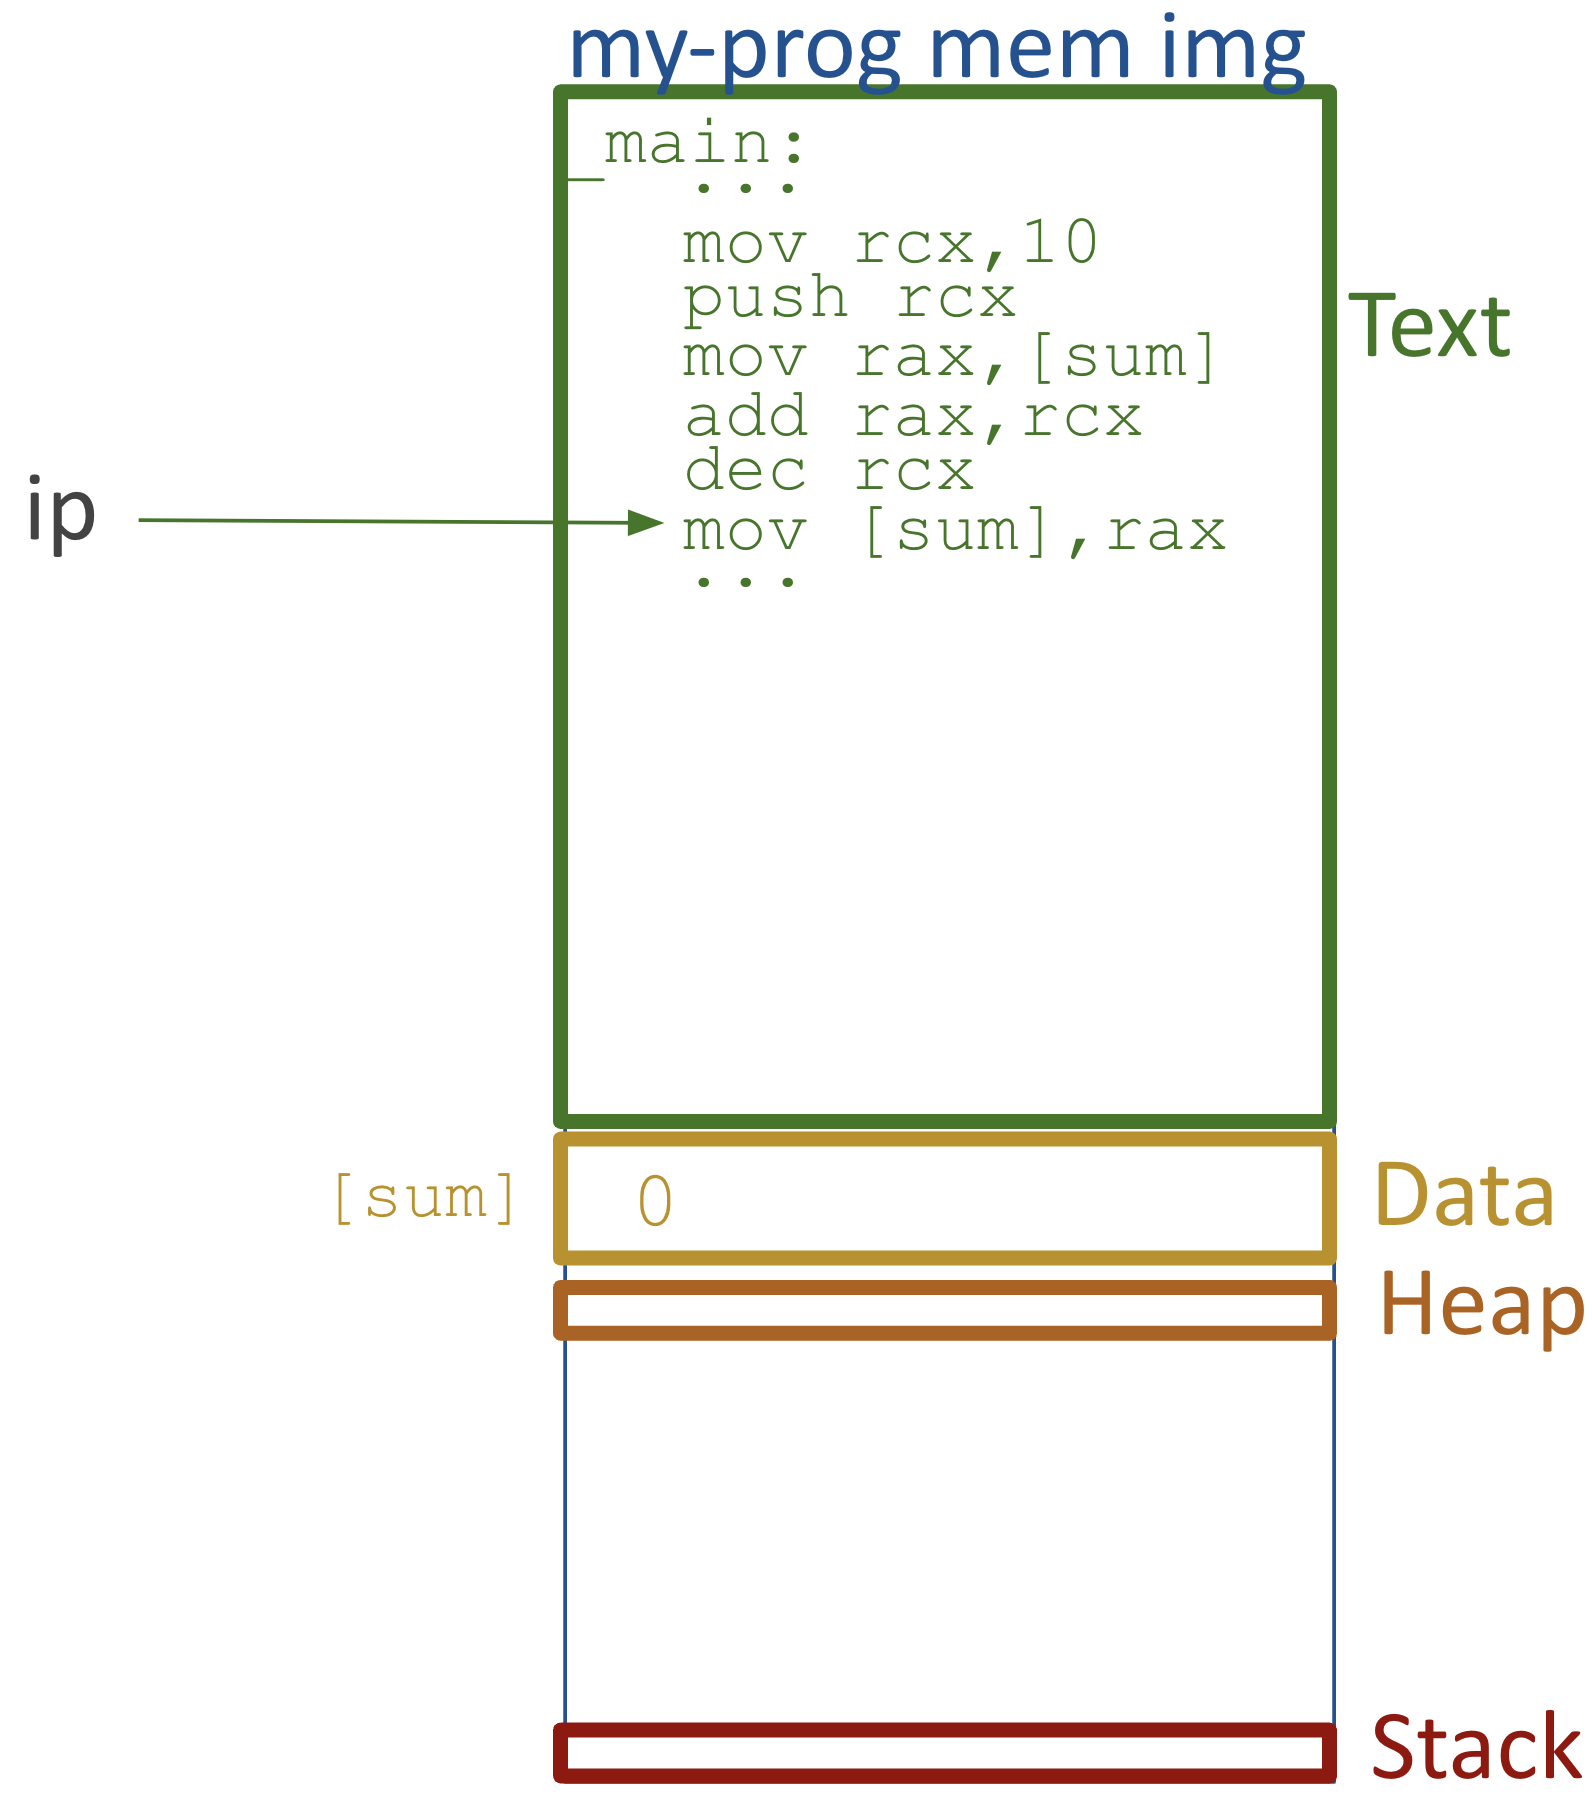
\includegraphics[width=0.75\textwidth]{chapters/L2/images/stack.png}
\end{center}
\end{minipage}

\subsubsection{Stack Frames}
Each function call creates its own \emph{stack frame}, a self-contained section that isolates the function's local data. This segmentation helps maintain the correct scope and lifetime for local variables and ensures that return addresses are preserved. The following diagram illustrates the organization of stack frames during nested function calls:

\begin{center}
    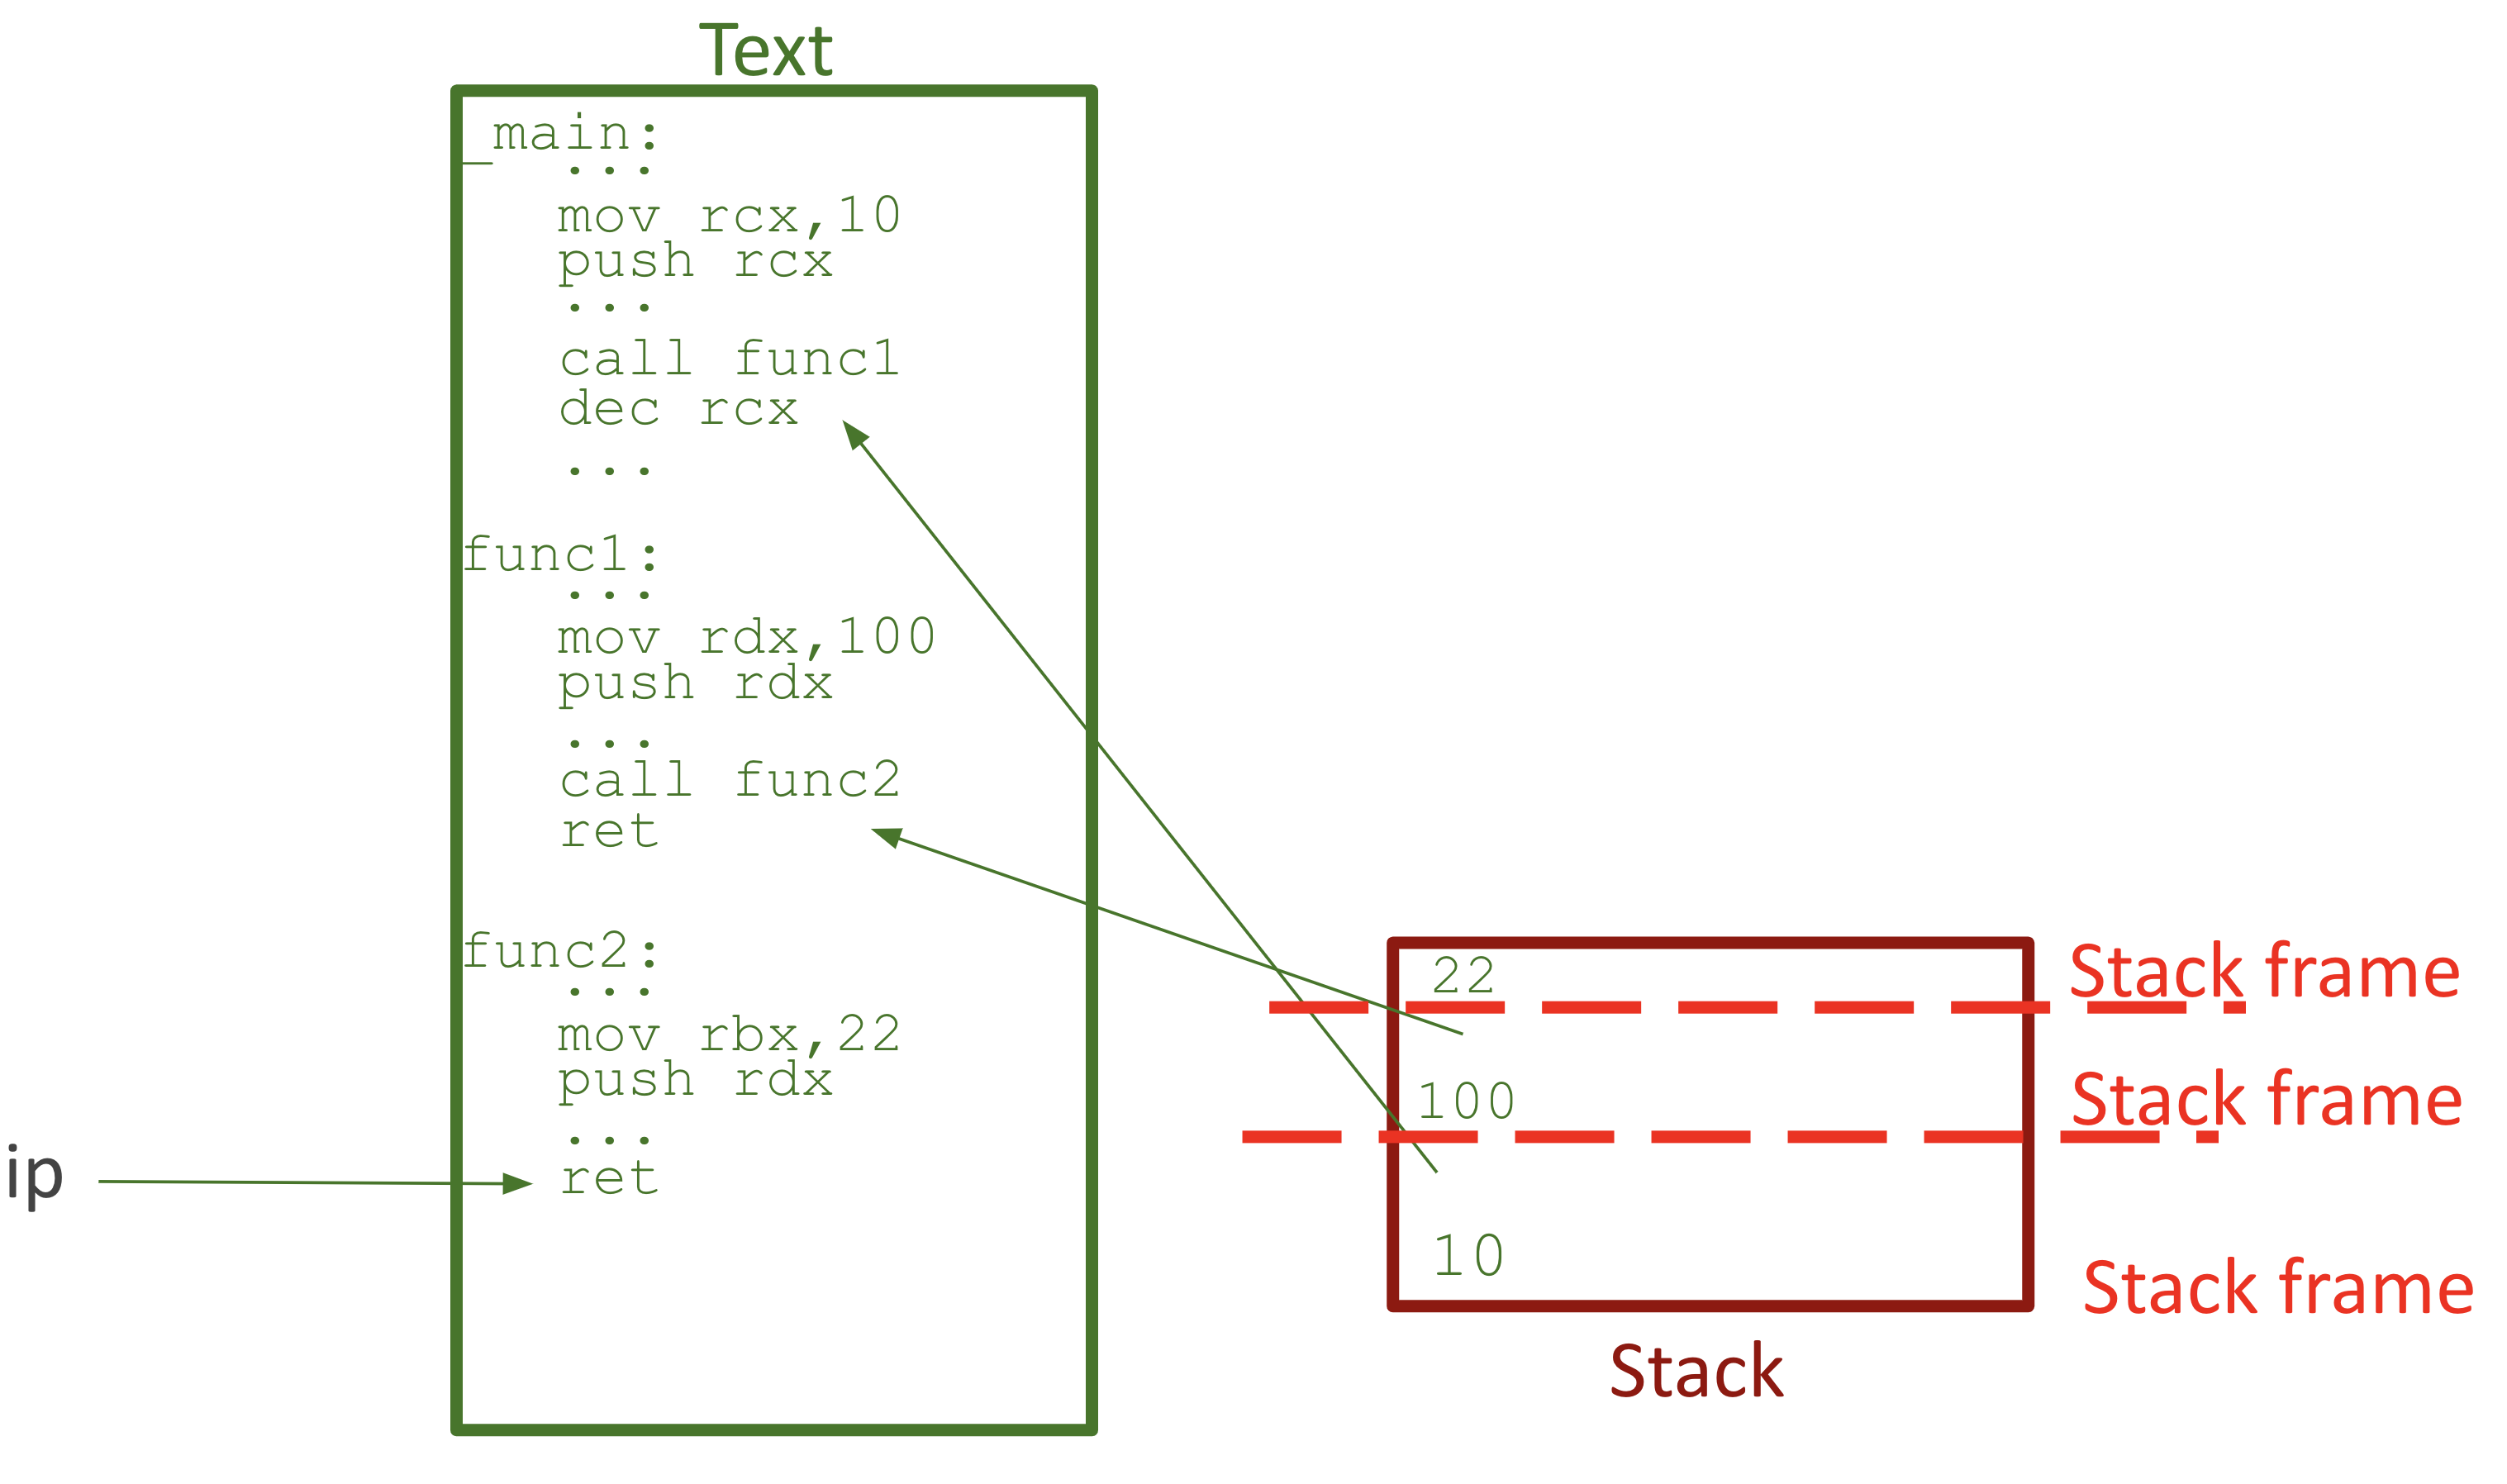
\includegraphics[width=0.65\textwidth]{chapters/L2/images/frames.png}
\end{center}

\subsection{Heap Memory}
The heap is used for dynamic memory allocation, where memory is allocated and deallocated as needed during runtime. Unlike the stack:
\begin{itemize}
  \item[-] \textbf{Manual vs. Automatic Management:} In languages such as C or C++, the programmer is responsible for explicitly allocating (using \texttt{malloc} or \texttt{new}) and deallocating (using \texttt{free} or \texttt{delete}) heap memory. In contrast, some modern languages employ automatic garbage collection.
  \item[-] \textbf{Growth Direction:} The heap typically grows upward, from lower to higher memory addresses.
  \item[-] \textbf{Lifetime:} Data allocated on the heap persists beyond the scope of the function that created it, until it is explicitly freed or garbage collected.
\end{itemize}

\subsection{Data and Text Segments}

\textbf{Text Segment:}  
This segment contains the program's executable code and constant values. Its read-only nature helps prevent inadvertent modifications during execution.
\vspace{0.5em}
\textbf{Data Segment:}  
This segment holds global and static variables. It is divided into:
\begin{itemize}
  \item[-] \textbf{Initialized Data:} Variables that have been assigned an initial value at compile time.
  \item[-] \textbf{Uninitialized Data (BSS):} Variables that are declared but not explicitly initialized; these are automatically set to zero at program startup.
\end{itemize}

\begin{definition}[CPU Registers]
Two registers are critical for process execution:
\begin{itemize}
  \item[-] \textbf{Instruction Pointer (IP):} Points to the next instruction in the text segment.
  \item[-] \textbf{Stack Pointer (SP):} Points to the top of the stack.
\end{itemize}
\end{definition}

\begin{definition}[Process and Thread Identifiers]
\leavevmode\\ % Ensures LaTeX enters vertical mode before inserting a newline
A process is considered to be \emph{running} if at least one of its threads is executing; otherwise, it is not running.
\begin{itemize}
  \item[-] \textbf{Process ID (PID):} A unique identifier assigned to each process.
  \item[-] \textbf{Thread ID (TID):} A unique identifier for each thread, which may be unique within a process or across the entire system, depending on the operating system.
\end{itemize}
\end{definition}

\begin{definition}[Resource Sharing]
Processes and threads share system resources such as CPU and memory. Each thread is given the illusion of having exclusive access to the CPU, and each process appears to have dedicated memory, even though these resources are actually shared.
\end{definition}
\vspace{10px}

\begin{definition}[CPU Sharing]
The CPU is time-shared among multiple threads. This virtualization is achieved through context switching, where the CPU rapidly switches between threads, giving each one the impression of exclusive use of the processor.
\end{definition}

\subsubsection{Example: Two Programs Running on a Single Core}
\begin{example}
Consider two programs running on a single-core processor. Each program is assigned a CPU context, which includes register values such as \texttt{rax}, \texttt{rbx}, the stack pointer (SP), and the instruction pointer (IP). When switching between programs, the CPU saves the current context to memory and loads the context of the next program, allowing the programs to resume correctly.
\end{example}

\begin{center}
    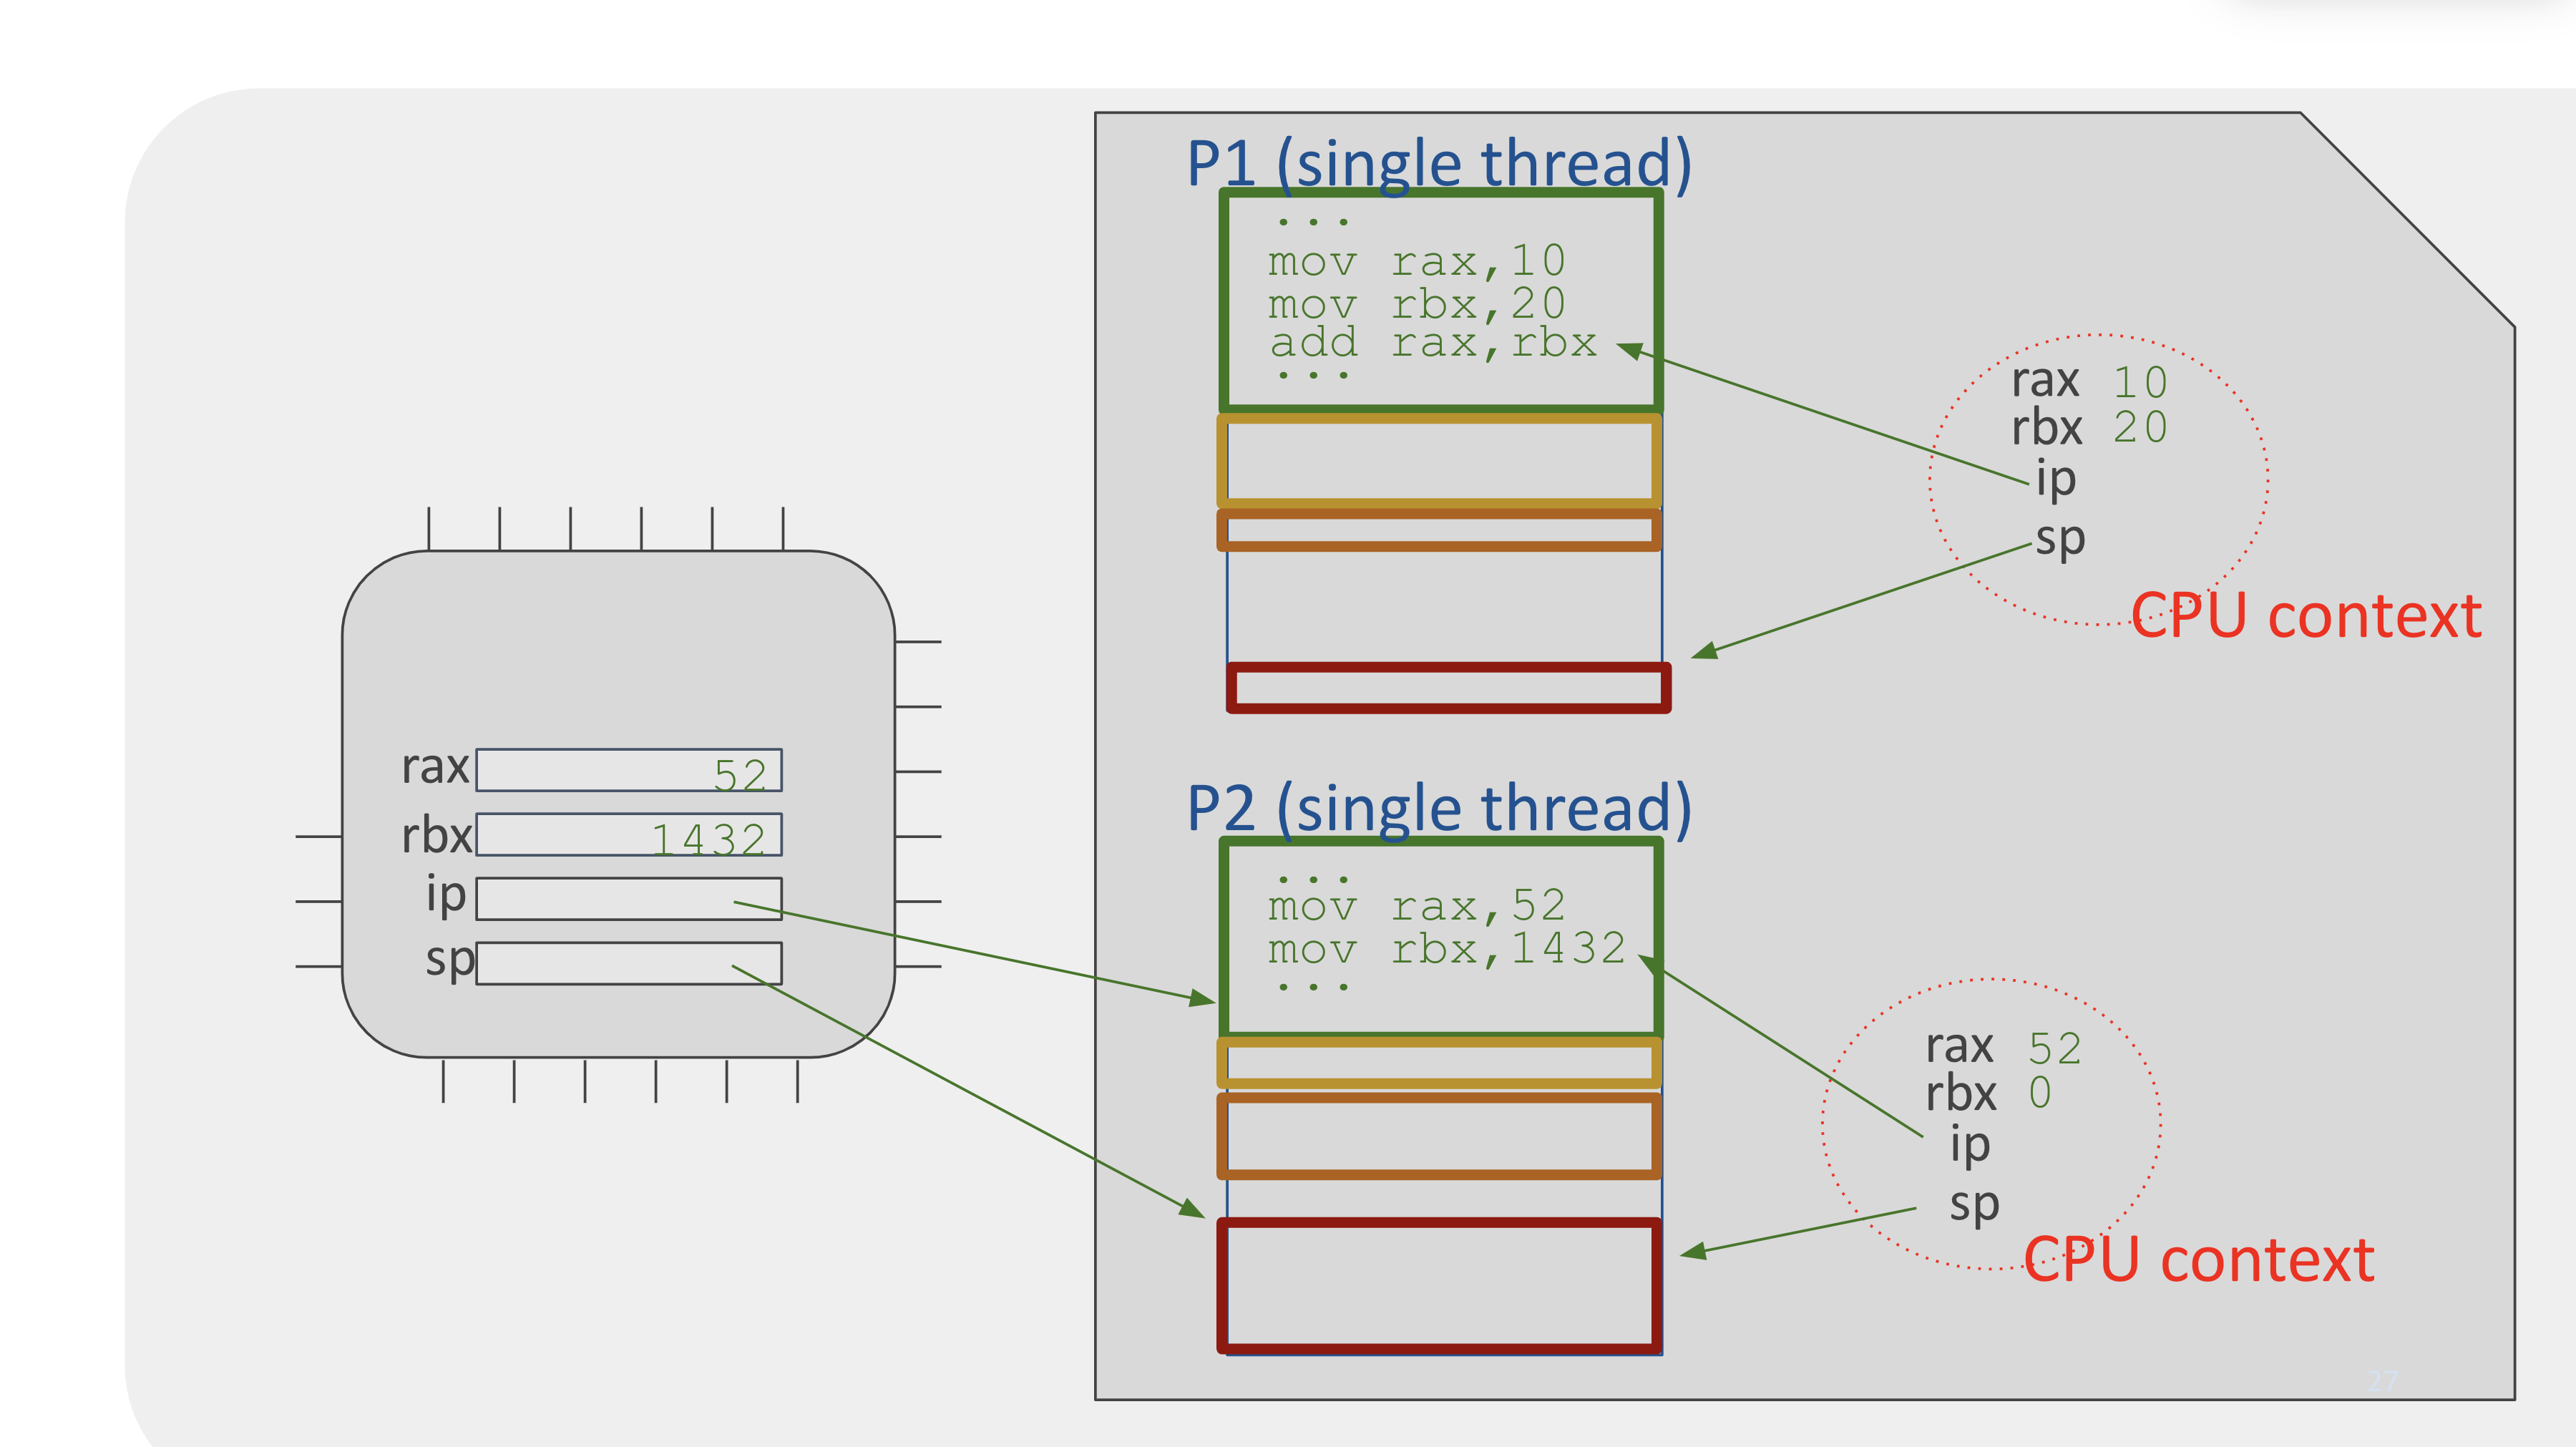
\includegraphics[width=0.8\textwidth]{chapters/L2/images/cpu_context.png}
\end{center}

\begin{definition}[Thread's CPU Context]
A thread's CPU context comprises the values of all CPU registers at the moment it was last executing. In a single-threaded process, this context represents the entire process state.
\end{definition}

\begin{definition}[Context Switching]
Context switching is the process by which the CPU switches from executing one thread to another. It involves:
\begin{enumerate}
    \item Saving the current thread's CPU context to memory.
    \item Restoring the CPU context of the thread to be executed next.
    \item[] Each thread has the illusion that it's occupying the CPU \textbf{alone}.
\end{enumerate}
This mechanism enables CPU virtualization but introduces performance overhead due to additional memory accesses.
\end{definition}
\vspace{10px}
\begin{definition}[Process]
A process is defined by:
\begin{itemize}
    \item A unique Process ID (PID).
    \item A memory image that includes the text, data, heap, and stack segments.
    \item The CPU contexts of each thread within the process.
    \item Associated resources such as file descriptors.
\end{itemize}
\end{definition}
\textit{Remark: If two threads belong to the same process, does each have its own CPU context, or do they share one? The answer is that each thread should be able to continue its execution independently.}
\vspace{10px}
\begin{definition}[Memory Sharing]
Memory in a system is space-shared among processes; however, virtualization ensures that each process operates within its own isolated address space. This is achieved through virtual-to-physical address translation.
\end{definition}
\vspace{10px}
\begin{definition}[Virtual and Physical Addresses]
Virtual addresses allow processes to operate as if they have exclusive access to memory. For example, two processes might both use the virtual address \texttt{0x400000}; however, these addresses map to different physical addresses:
\begin{itemize}
  \item[-] Process \( P_1 \): Virtual \texttt{0x400000} \(\rightarrow\) Physical \texttt{0x1234AFF8}
  \item[-] Process \( P_2 \): Virtual \texttt{0x400000} \(\rightarrow\) Physical \texttt{0xABCD5678}
\end{itemize}
\end{definition}
\vspace{10px}
\begin{definition}[Virtual Address Space]
Each process is allocated its own virtual address space, which is shared among all its threads. This abstraction allows developers to ignore the complexities of physical memory allocation.
\end{definition}
\vspace{10px}
\begin{definition}[Address Translation]
Address translation is the process by which a virtual memory address is converted into a physical memory address. While essential for memory virtualization, this translation incurs a performance cost.
\end{definition}

\subsection{Stack Smashing}
Stack smashing is a type of buffer overflow vulnerability where an attacker deliberately overwrites parts of the memory on the call stack. This typically happens when a program writes more data into a fixed-size buffer than it can accommodate, thereby corrupting adjacent memory areas such as the function's return address.

\paragraph{How It Works:}
When a function is called, a stack frame is created that contains local variables, return addresses, and other control data. If a buffer does not have proper bounds checking, an input exceeding the buffer's capacity can overflow into these critical areas. For example:
\begin{enumerate}
    \item A fixed-size buffer is allocated on the stack.
    \item Excess input data overwrites memory beyond the buffer.
    \item The return address (or other control data) is corrupted.
    \item On function return, control is transferred to an address chosen by the attacker, potentially executing malicious code.
\end{enumerate}
\subsection{Summary: CPU and Memory Virtualization}
\begin{itemize}
    \item \textbf{CPU Virtualization:} Threads time-share the CPU through context switching, which gives each thread the illusion of exclusive CPU access.
    \item \textbf{Memory Virtualization:} Processes space-share memory via virtual-to-physical address translation, ensuring that each process operates in its own isolated address space.
\end{itemize}

\subsection{Conclusion}
Modern operating systems are designed to enable multiple programs to share CPU and memory resources seamlessly. Through context switching and address translation, both the CPU and memory are effectively virtualized. This abstraction simplifies development, as compilers and developers can design programs without needing to manage these low-level resource-sharing details directly.


 
\chapter{L3 - Sharing the CPU}

This chapter introduces the mechanisms by which an operating system (OS) manages access to the CPU, ensuring both security and fairness among processes. We discuss CPU privilege levels, the limited direct execution model, and the role of system calls (syscalls) in process management.
\vfill
\section{The OS as a Special Program}

The operating system (OS) is a fundamental software layer that manages hardware resources and provides essential services for user applications. Unlike typical applications, the OS operates at different privilege levels and ensures secure and efficient execution of processes and threads.
\subsection{Limited Direct Execution}
\textbf{Professor Analogy cont. -} The children have direct access to the TV but are restricted by Kids Mode. \\
Limited direct execution is a method that allows a thread to run directly on the CPU while enforcing certain restrictions:
\begin{itemize}
  \item[-] \emph{Direct Execution:} The CPU executes the thread's instructions without any intermediate emulation.
  \item[-] \emph{Limited:} The thread cannot perform operations that require high privileges; instead, it must request system assistance via syscalls.
\end{itemize}
The CPU runs in Limited Direct Execution. Let's see how it's limited 
\newpage
\subsection{CPU Privilege Levels and Execution Modes}
\textbf{Professor Analogy -} Imagine you have children who want to watch TV. You can either keep the remote with you and ask them to call you whenever they need to change the channel, or you can enable Kids Mode on the TV, allowing them limited access without needing to ask for permission each time. \\[3px]
\textit{Personal Remark - Kernal code \emph{always} run in High Privilege mode, and because of this we say that the OS \emph{may} run in High Privilege mode (kernel is inside of the os), do not confuse both !}\\[3px]
The OS shares the CPU and main memory with normal user processes and threads. However, its execution mode differs based on its role at any given time:

\begin{itemize}
  \item[-] When the OS executes, the CPU \textit{may} be in \textbf{high privilege mode} (often called kernel mode), allowing it unrestricted access to all system resources.
\item[-] When a normal process or thread executes, the CPU is in \textbf{low privilege mode} (user mode), restricting access to critical system resources.
\end{itemize}

\begin{center}
  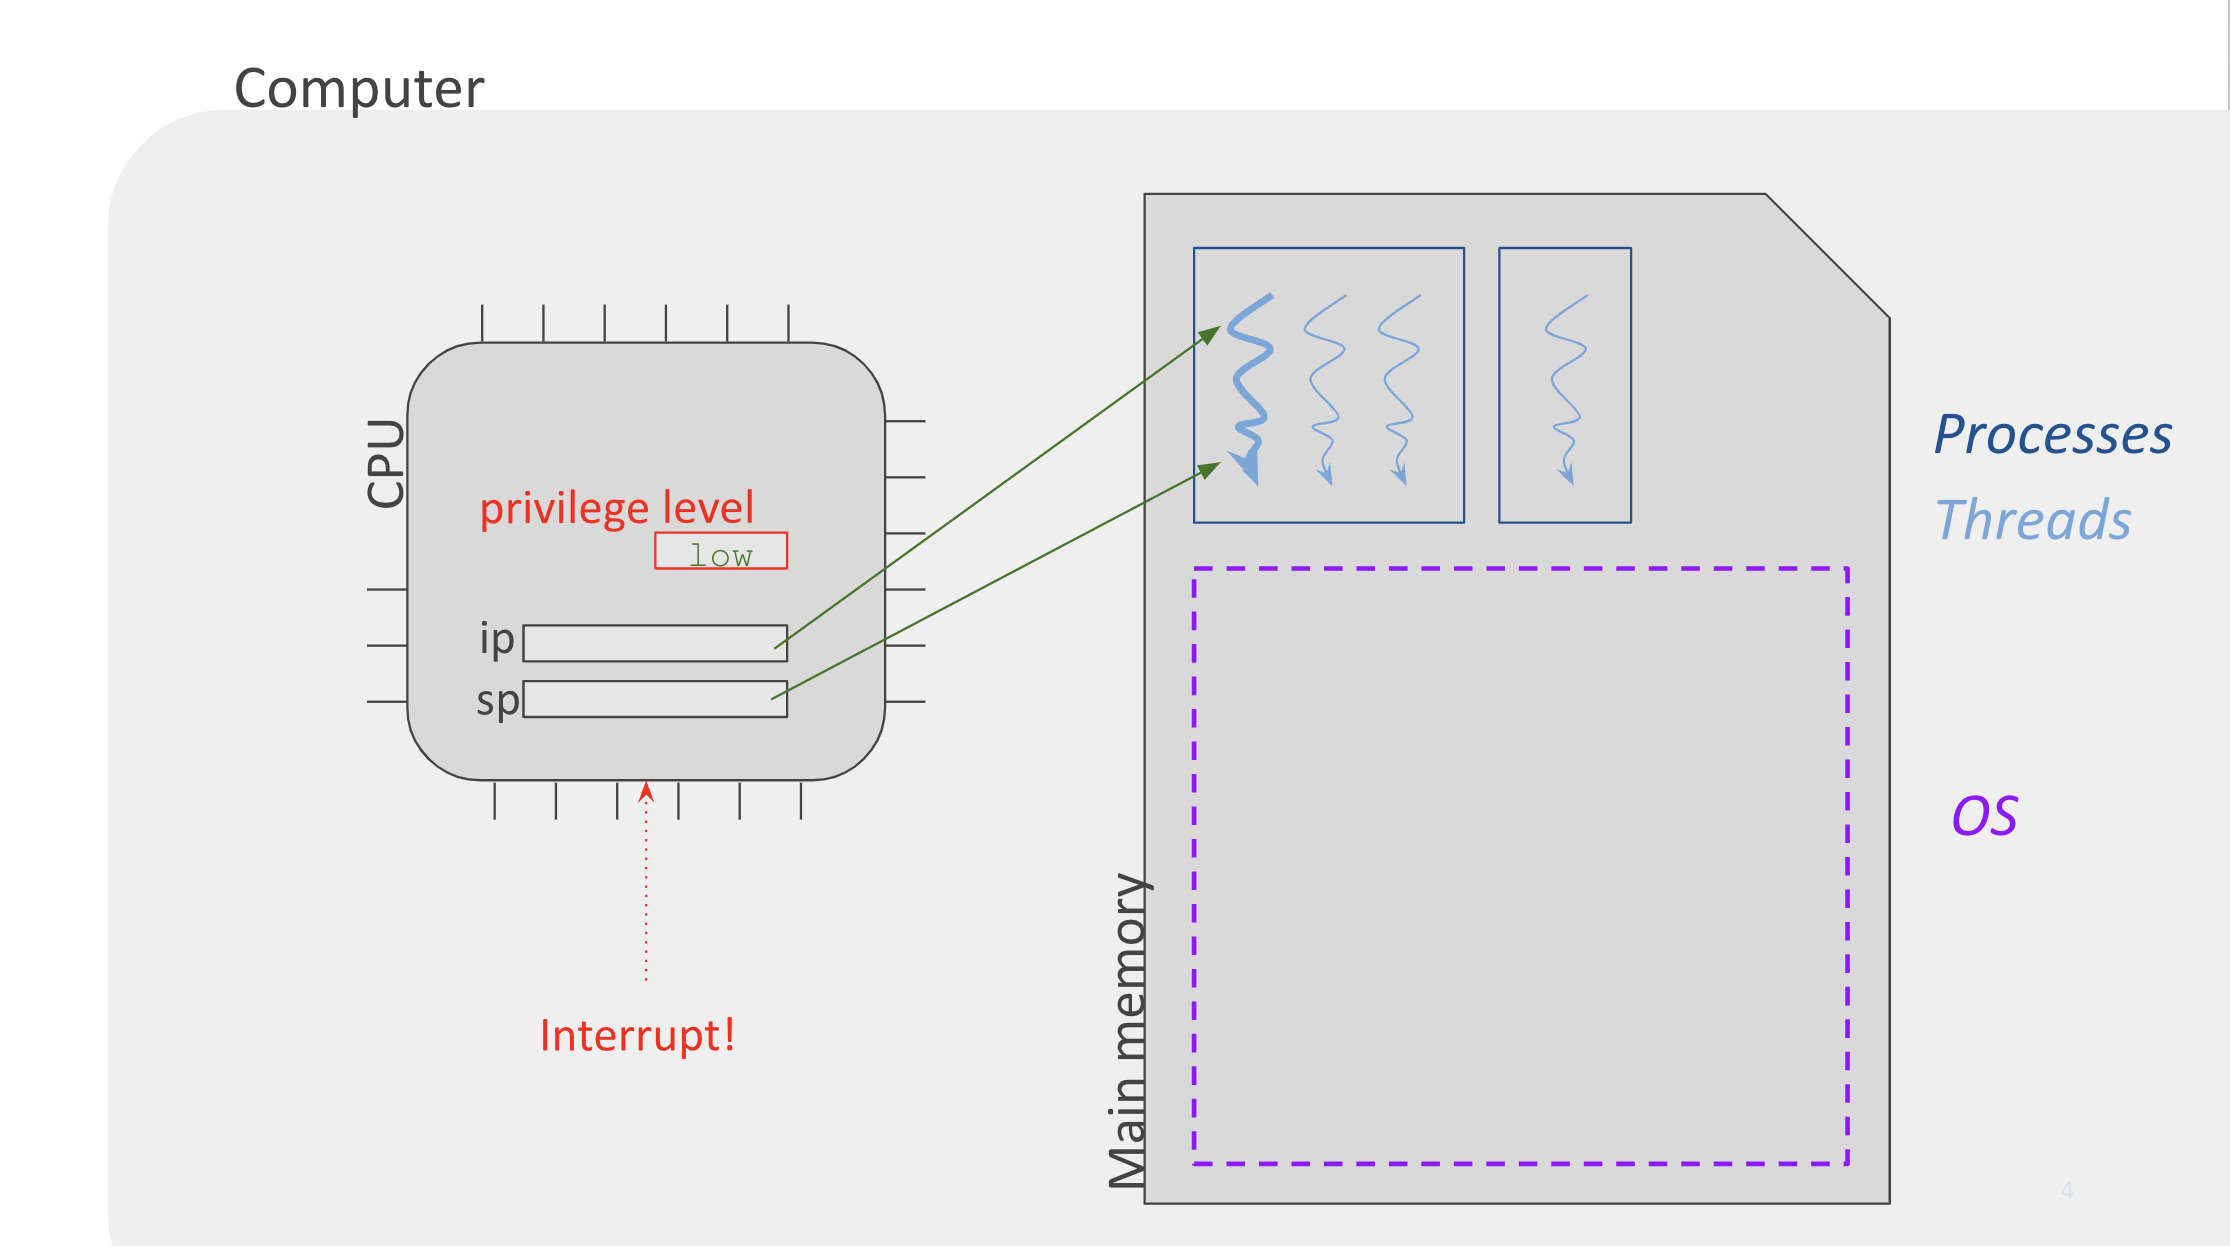
\includegraphics[width=0.8\textwidth]{chapters/L3/images/priviledge.png}
\end{center}

This privilege system exists primarily for security reasons, enforcing the \textbf{principle of least privilege}, where each process has only the necessary access rights required to perform its task. 

\subsection{The Kernel: Core Component of the OS}

A key component of the OS is the \textbf{kernel}, responsible for:

\begin{itemize}
  \item[-] Creating and managing processes and threads.
  \item[-] Allocating system resources (CPU time, memory, I/O devices, etc.).
  \item[-] Ensuring that each process has a designated portion of memory, including stack, data, and text segments.
  \item[-] Enforcing security and isolation between processes.
\end{itemize}

The kernel always runs in \textbf{high privilege mode} (kernel mode), which is why this mode is sometimes referred to as \textit{kernel mode}. 

\subsection{Process Management and Context Switching}

The OS does not execute continuously but rather runs only when necessary. It performs essential tasks, prepares the environment for the next process, and then switches out, allowing user processes to execute.

\begin{itemize}
  \item[-] The OS uses \textbf{context switching} to transition between processes efficiently, preserving the state of the current process before switching to another.
  \item[-] By switching between kernel mode and user mode, the OS ensures that user applications run securely and do not directly manipulate hardware resources.
\end{itemize}

\subsection*{The Loader: Setting Up Process Memory}

Another critical component of the OS is the \textbf{loader}, which is responsible for preparing a program for execution: \\
\begin{minipage}{0.45\textwidth}
\begin{itemize}
    \item[-] The loader completes the setup of the process's memory image.
    \item[-] It copies the command-line arguments used to launch the program (e.g., \texttt{ls -a}, where \texttt{-a} is an argument).
    \item[-] These arguments are stored in the \textbf{stack} of the main thread of the new process to ensure accessibility.
\end{itemize}
\end{minipage} \hfill \vline \hfill 
\begin{minipage}{0.45\textwidth}
If these arguments were stored in the loader's stack instead, the process would not be able to access them after execution begins.
\begin{center}
    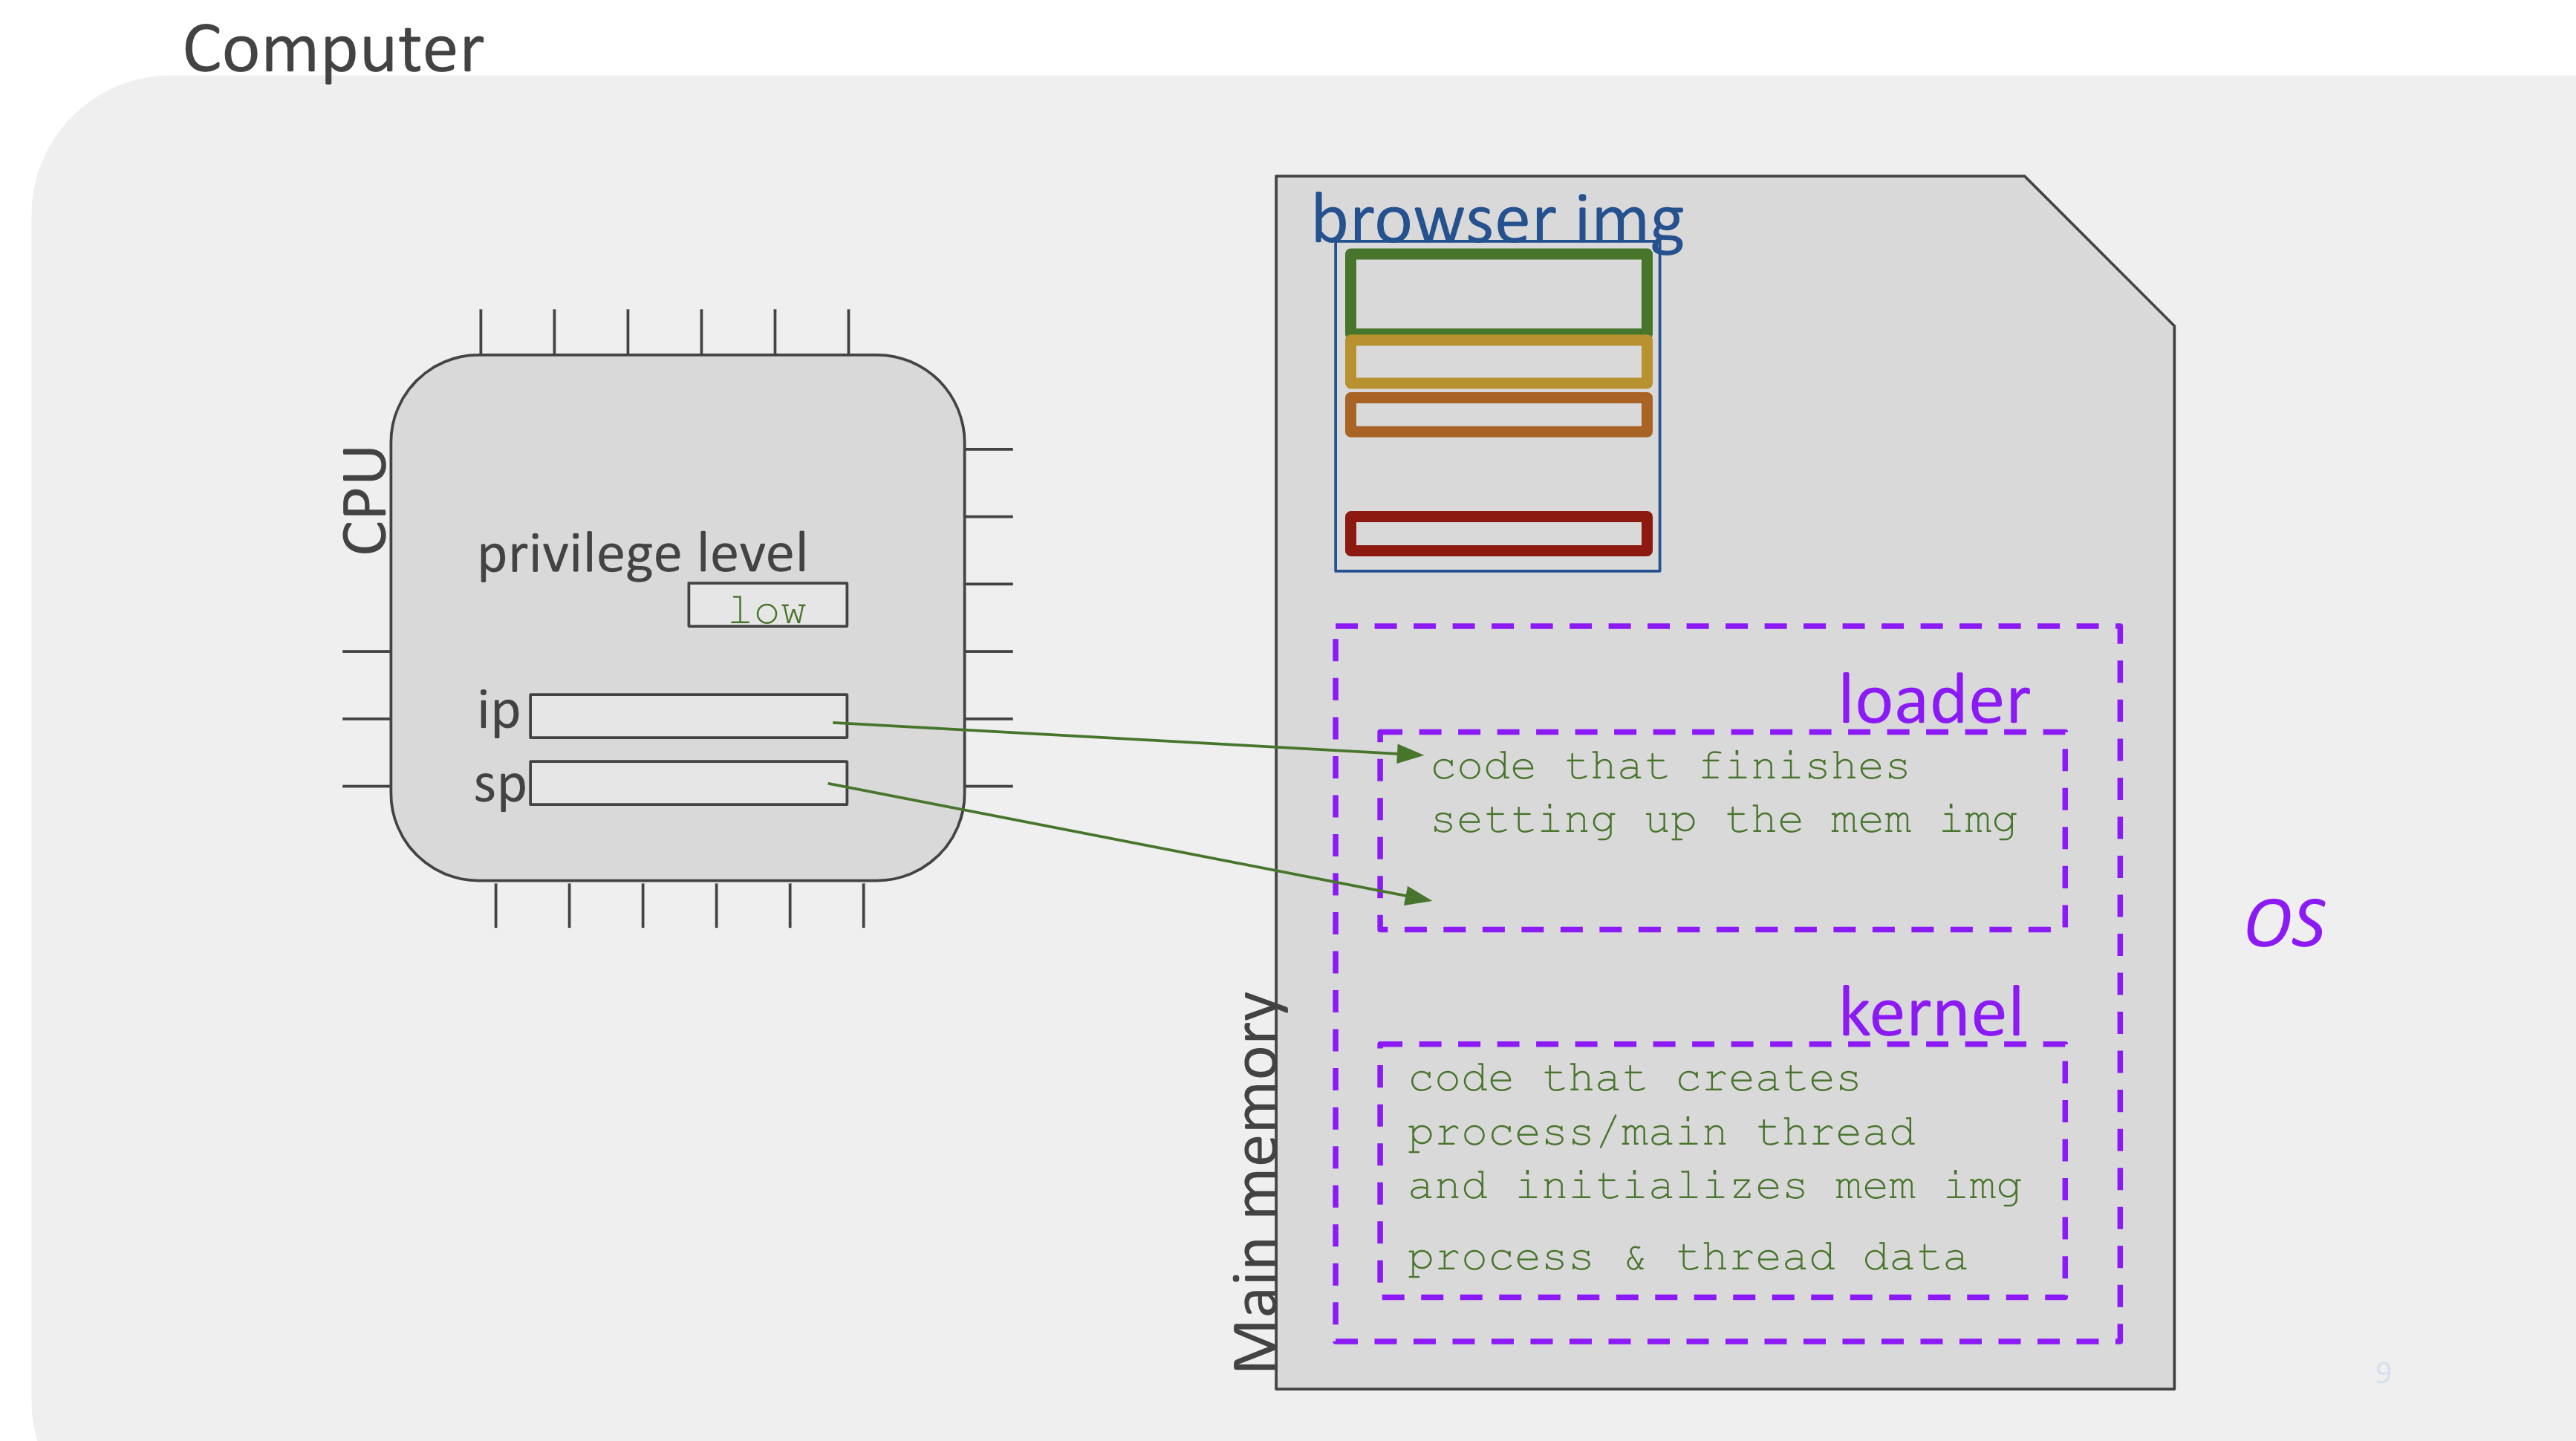
\includegraphics[width=1.1\textwidth]{chapters/L3/images/kernel.png}
\end{center}
\end{minipage} \\[10px]

This layered privilege model ensures a secure and efficient execution environment, maintaining stability and protection across all processes within the system.
\subsection{Syscalls}
\textit{Personal Remark - Syscalls are NOT needed when executing OS code, they only allow to cross the priviledged barrier when running a unpriviledged code.}
A \emph{syscall} is the mechanism by which a user process requests services from the OS. When a syscall is invoked:
\begin{enumerate}
  \item The CPU temporarily elevates the privilege level.
  \item The control is transferred to the OS to execute the privileged code.
  \item If the syscall involves an I/O operation, the process may be blocked while waiting for a response, and the CPU may perform a context switch to another thread.
  \item Once the operation is complete, the CPU returns to low privilege.
\end{enumerate}

\begin{center}
  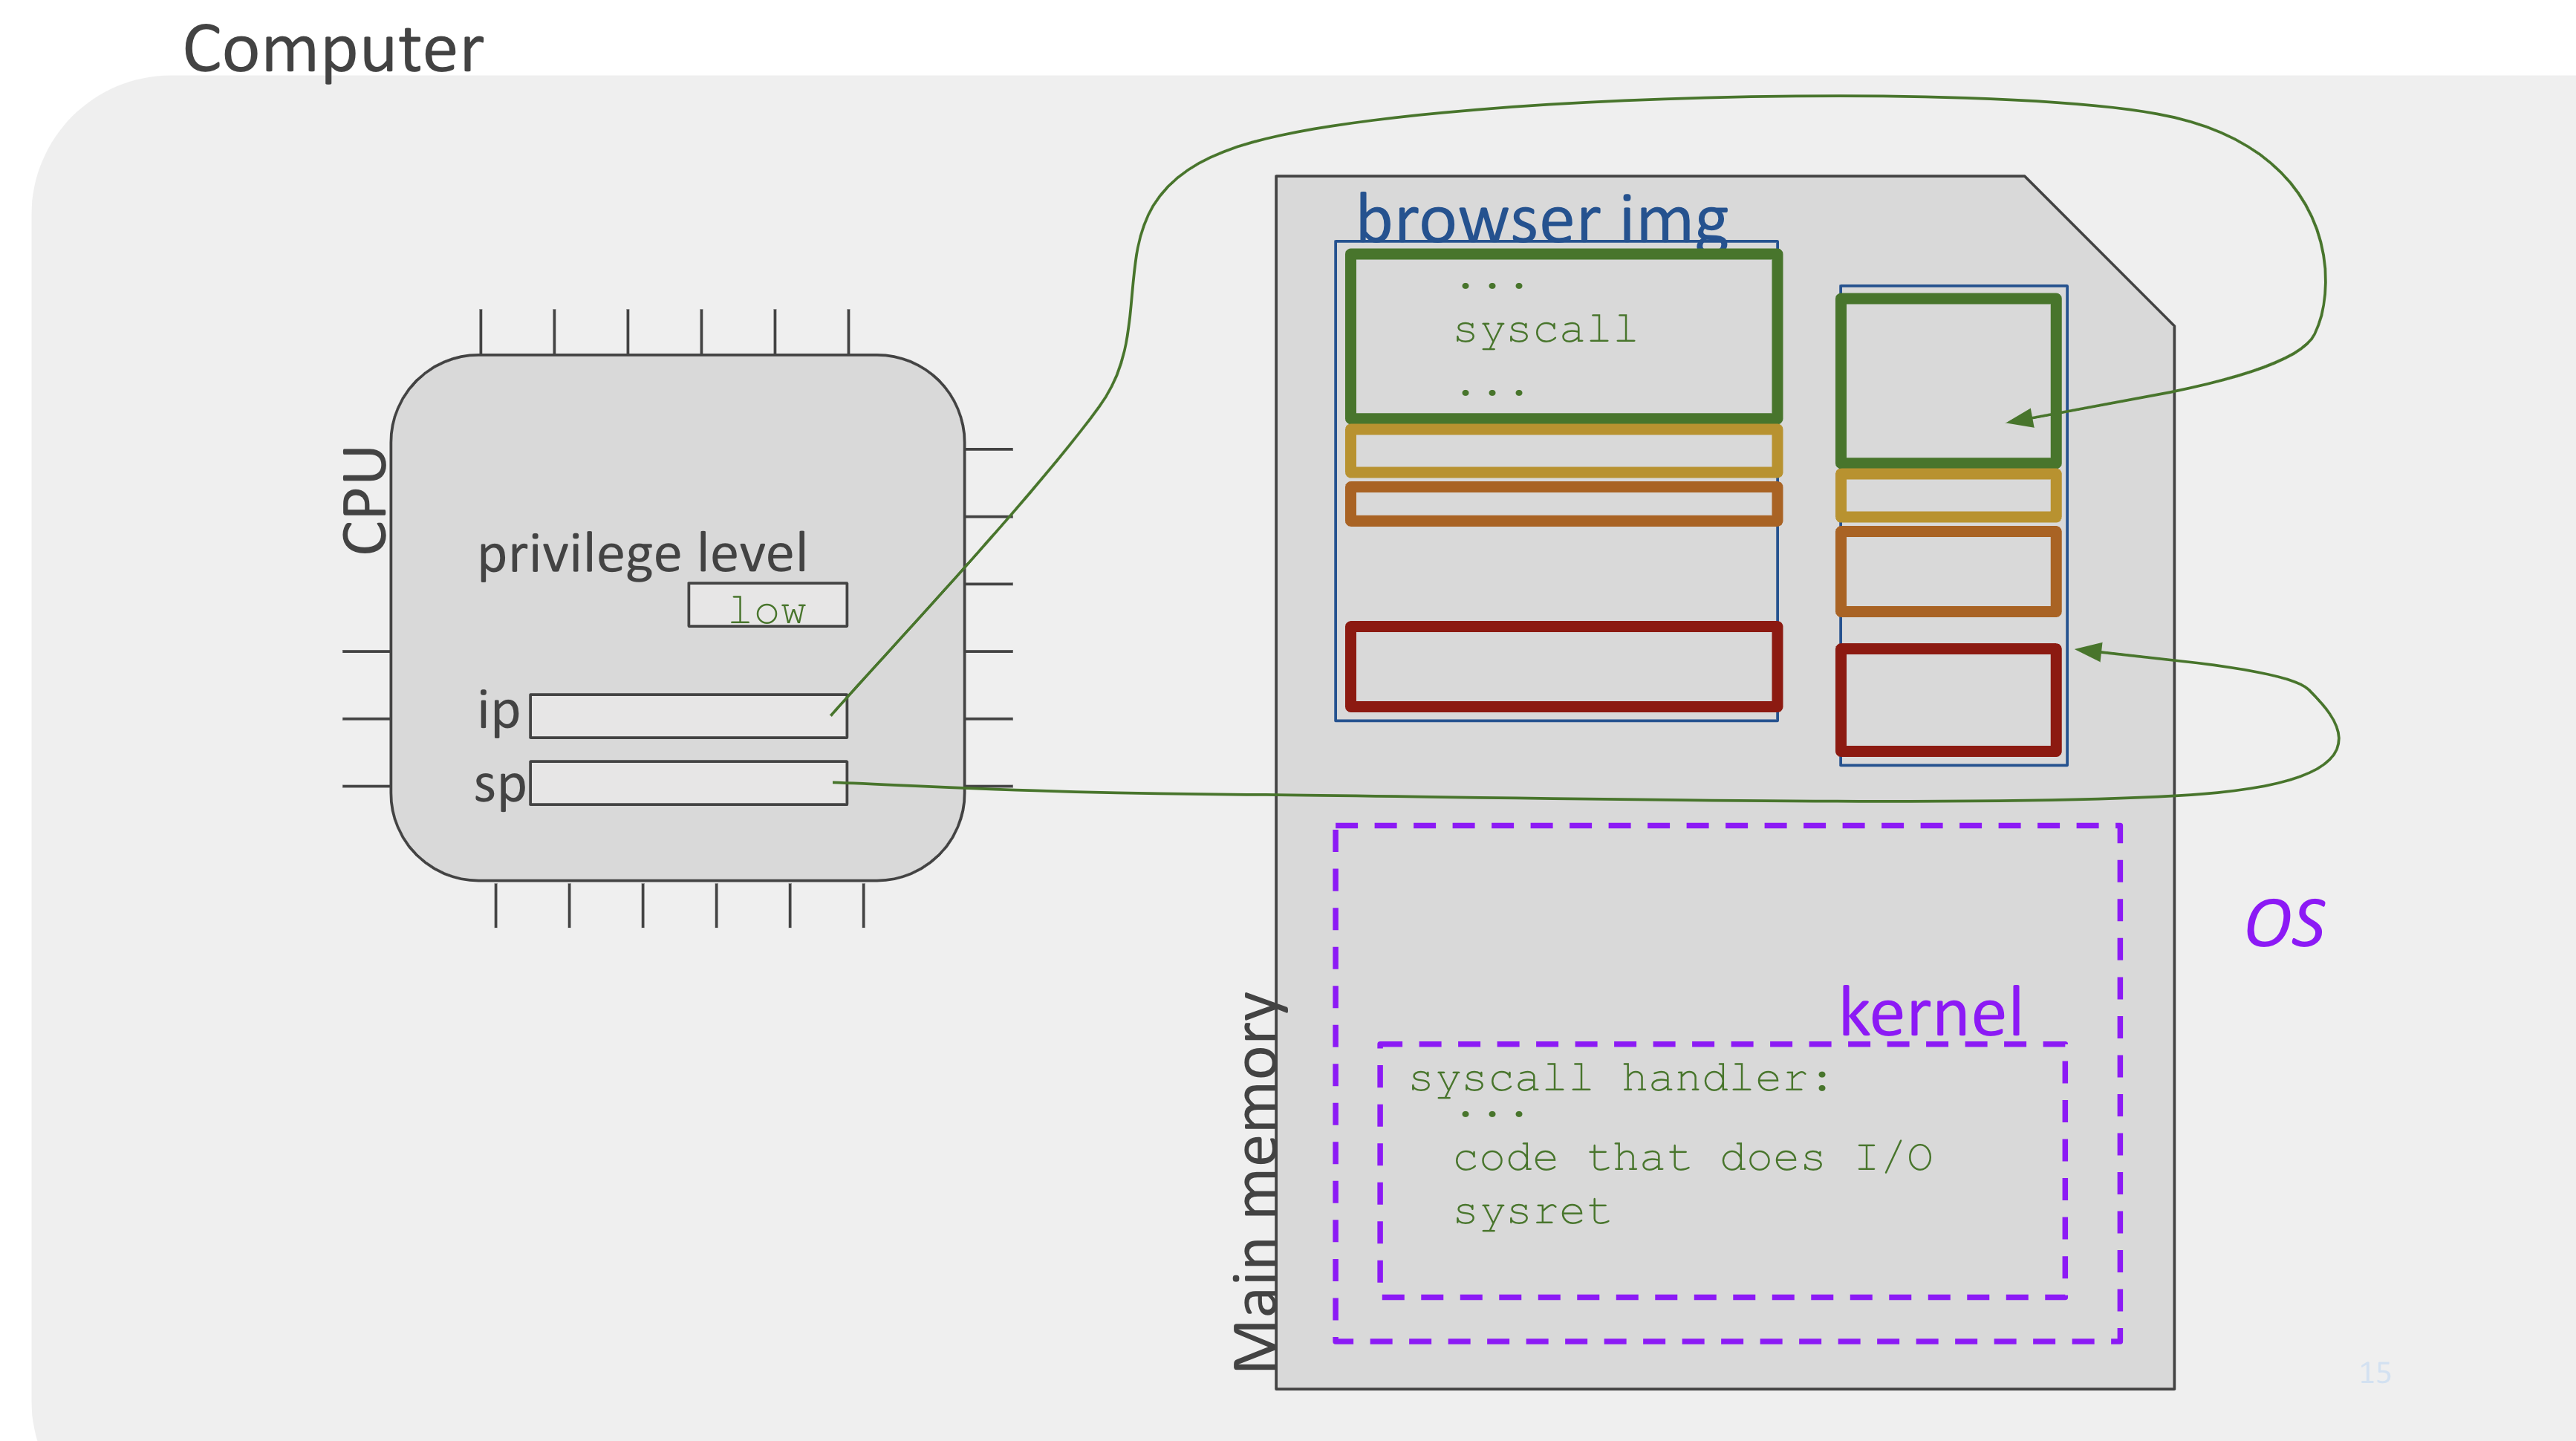
\includegraphics[width=0.8\textwidth]{chapters/L3/images/parallel-syscall.png}
\end{center}
\newpage
\subsection{Process I/O and Scheduling}
When a process initiates an I/O operation:\\
\begin{minipage}[htp]{0.45\textwidth}
\begin{itemize}
  \item It transitions from \emph{Running} to \emph{Blocked} as it waits for the I/O to complete.
  \item Once the I/O is complete, the process moves to the \emph{Ready} state.
  \item The OS scheduler then selects processes from the Ready queue to run, ensuring fair CPU utilization.
\end{itemize}
\end{minipage} 
\hfill 
\vline 
\hfill 
\begin{minipage}[htp]{0.45\textwidth}
\begin{center}
  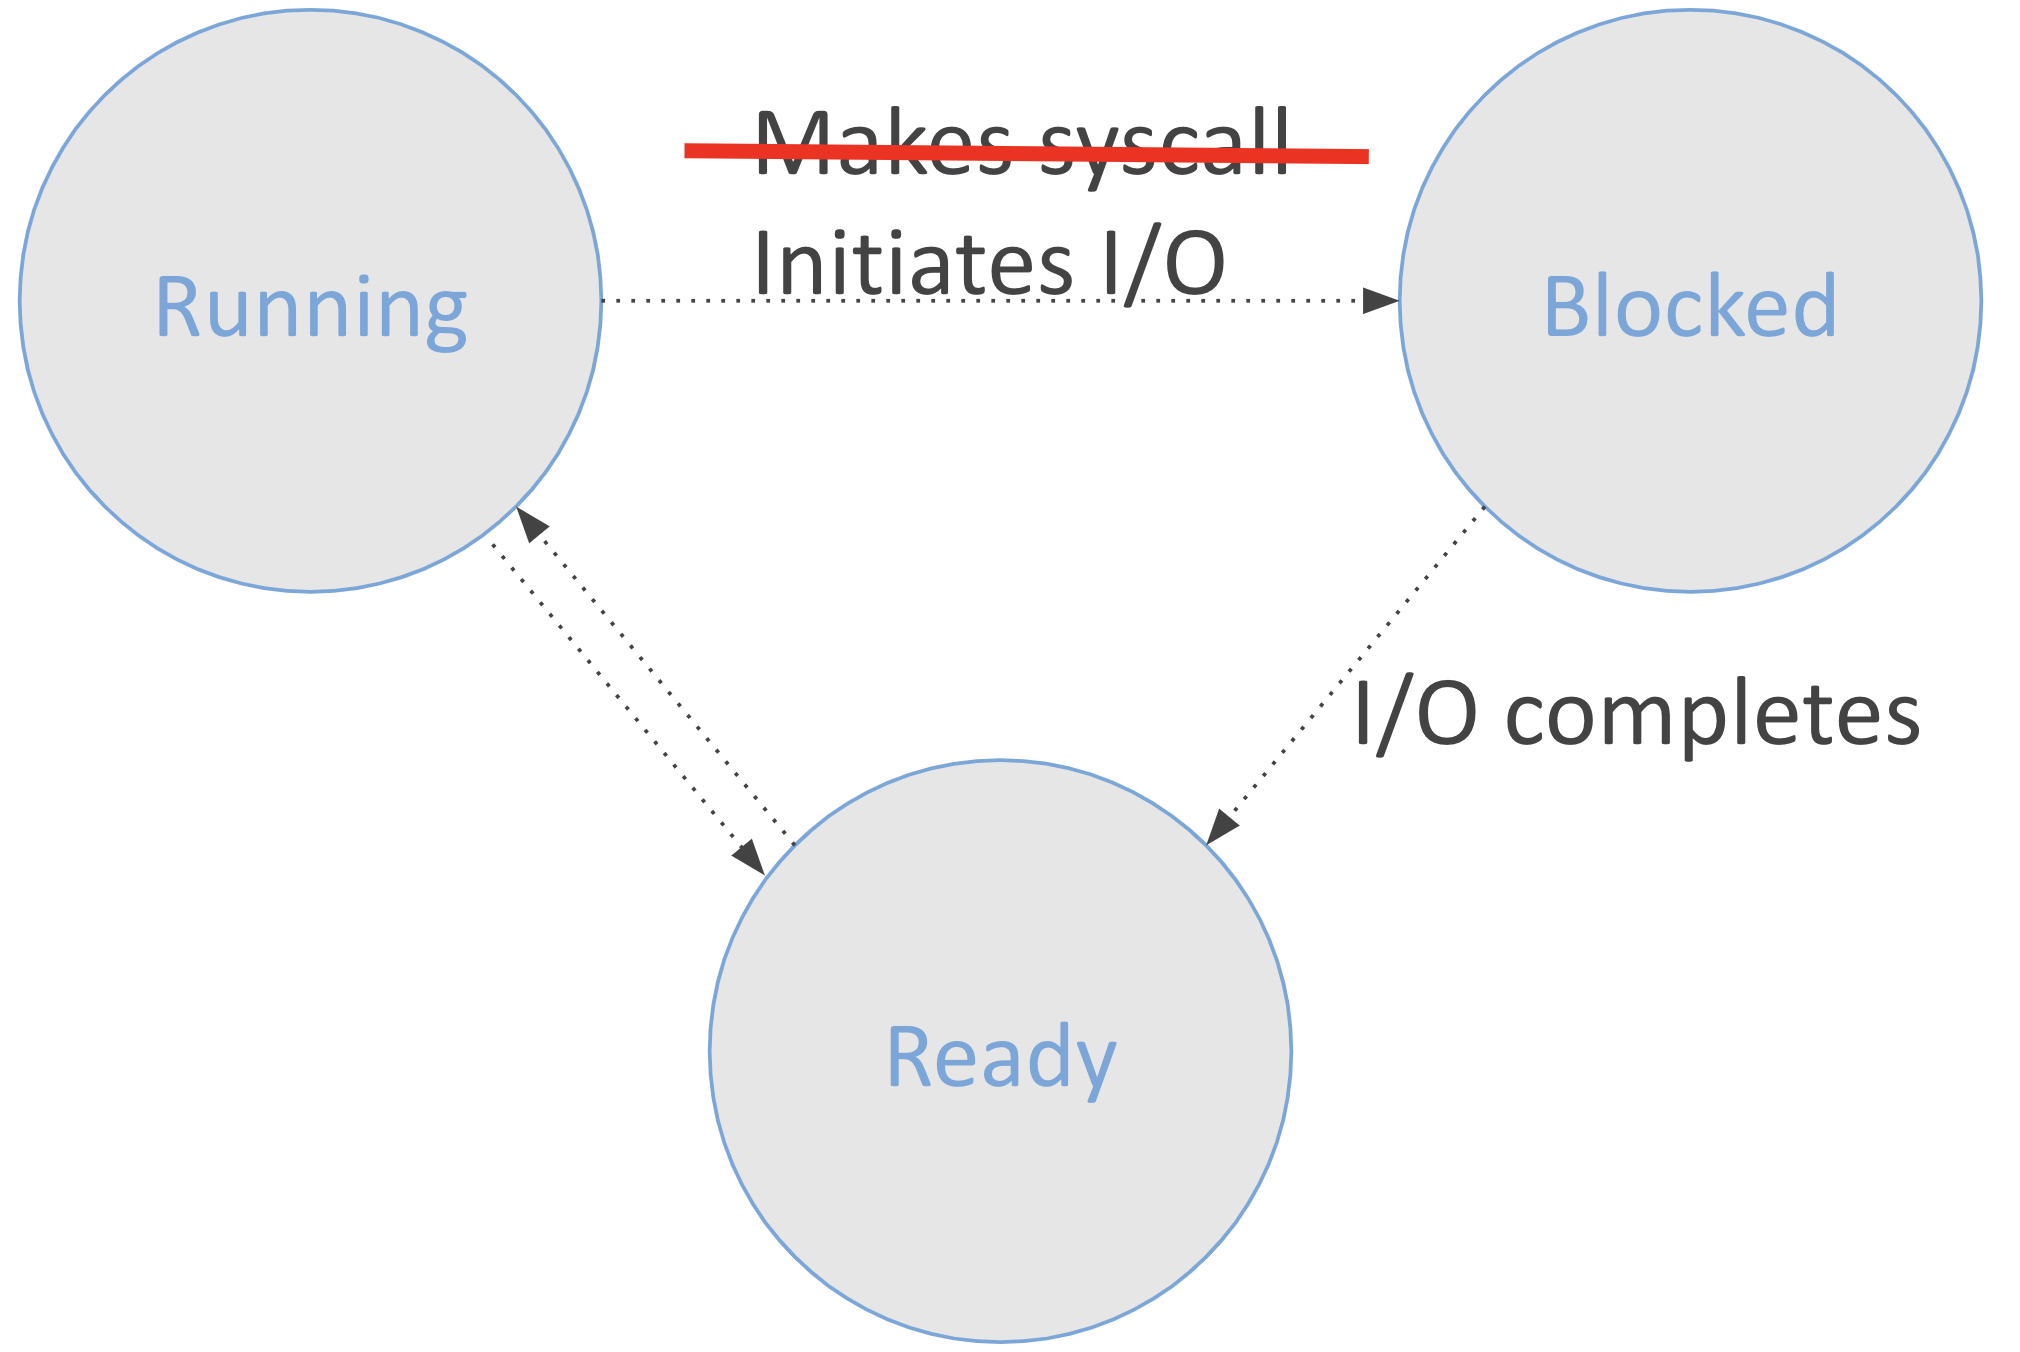
\includegraphics[width=0.95\textwidth]{chapters/L3/images/diagram.png}
\end{center}
\end{minipage}
\vspace{20px}
\section{The Kernel's Job cont.}
The Kernel handles several types of events:
\begin{itemize}[topsep=3px]
  \item[-] \textbf{Syscalls:} Requests from running threads for system-level services.
  \item[-] \textbf{Exceptions/Traps:} Synchronous signals generated when a thread executes an illegal or erroneous operation (e.g., division by zero).
  \item[-] \textbf{Interrupts:} Asynchronous signals from external devices (e.g., mouse events, network packets) requiring immediate attention.
\end{itemize}
\vspace{10px}
\begin{minipage}[htp]{0.45\textwidth}
\subsubsection*{Exception Handling}
\textit{What happens if the browser executes unauthorized code or encounters an error, such as dividing by zero ?}\\
When a process executes an illegal operation, the CPU raises an exception. The kernel then takes over to handle the error safely.
\vspace{8px}
\begin{center}
  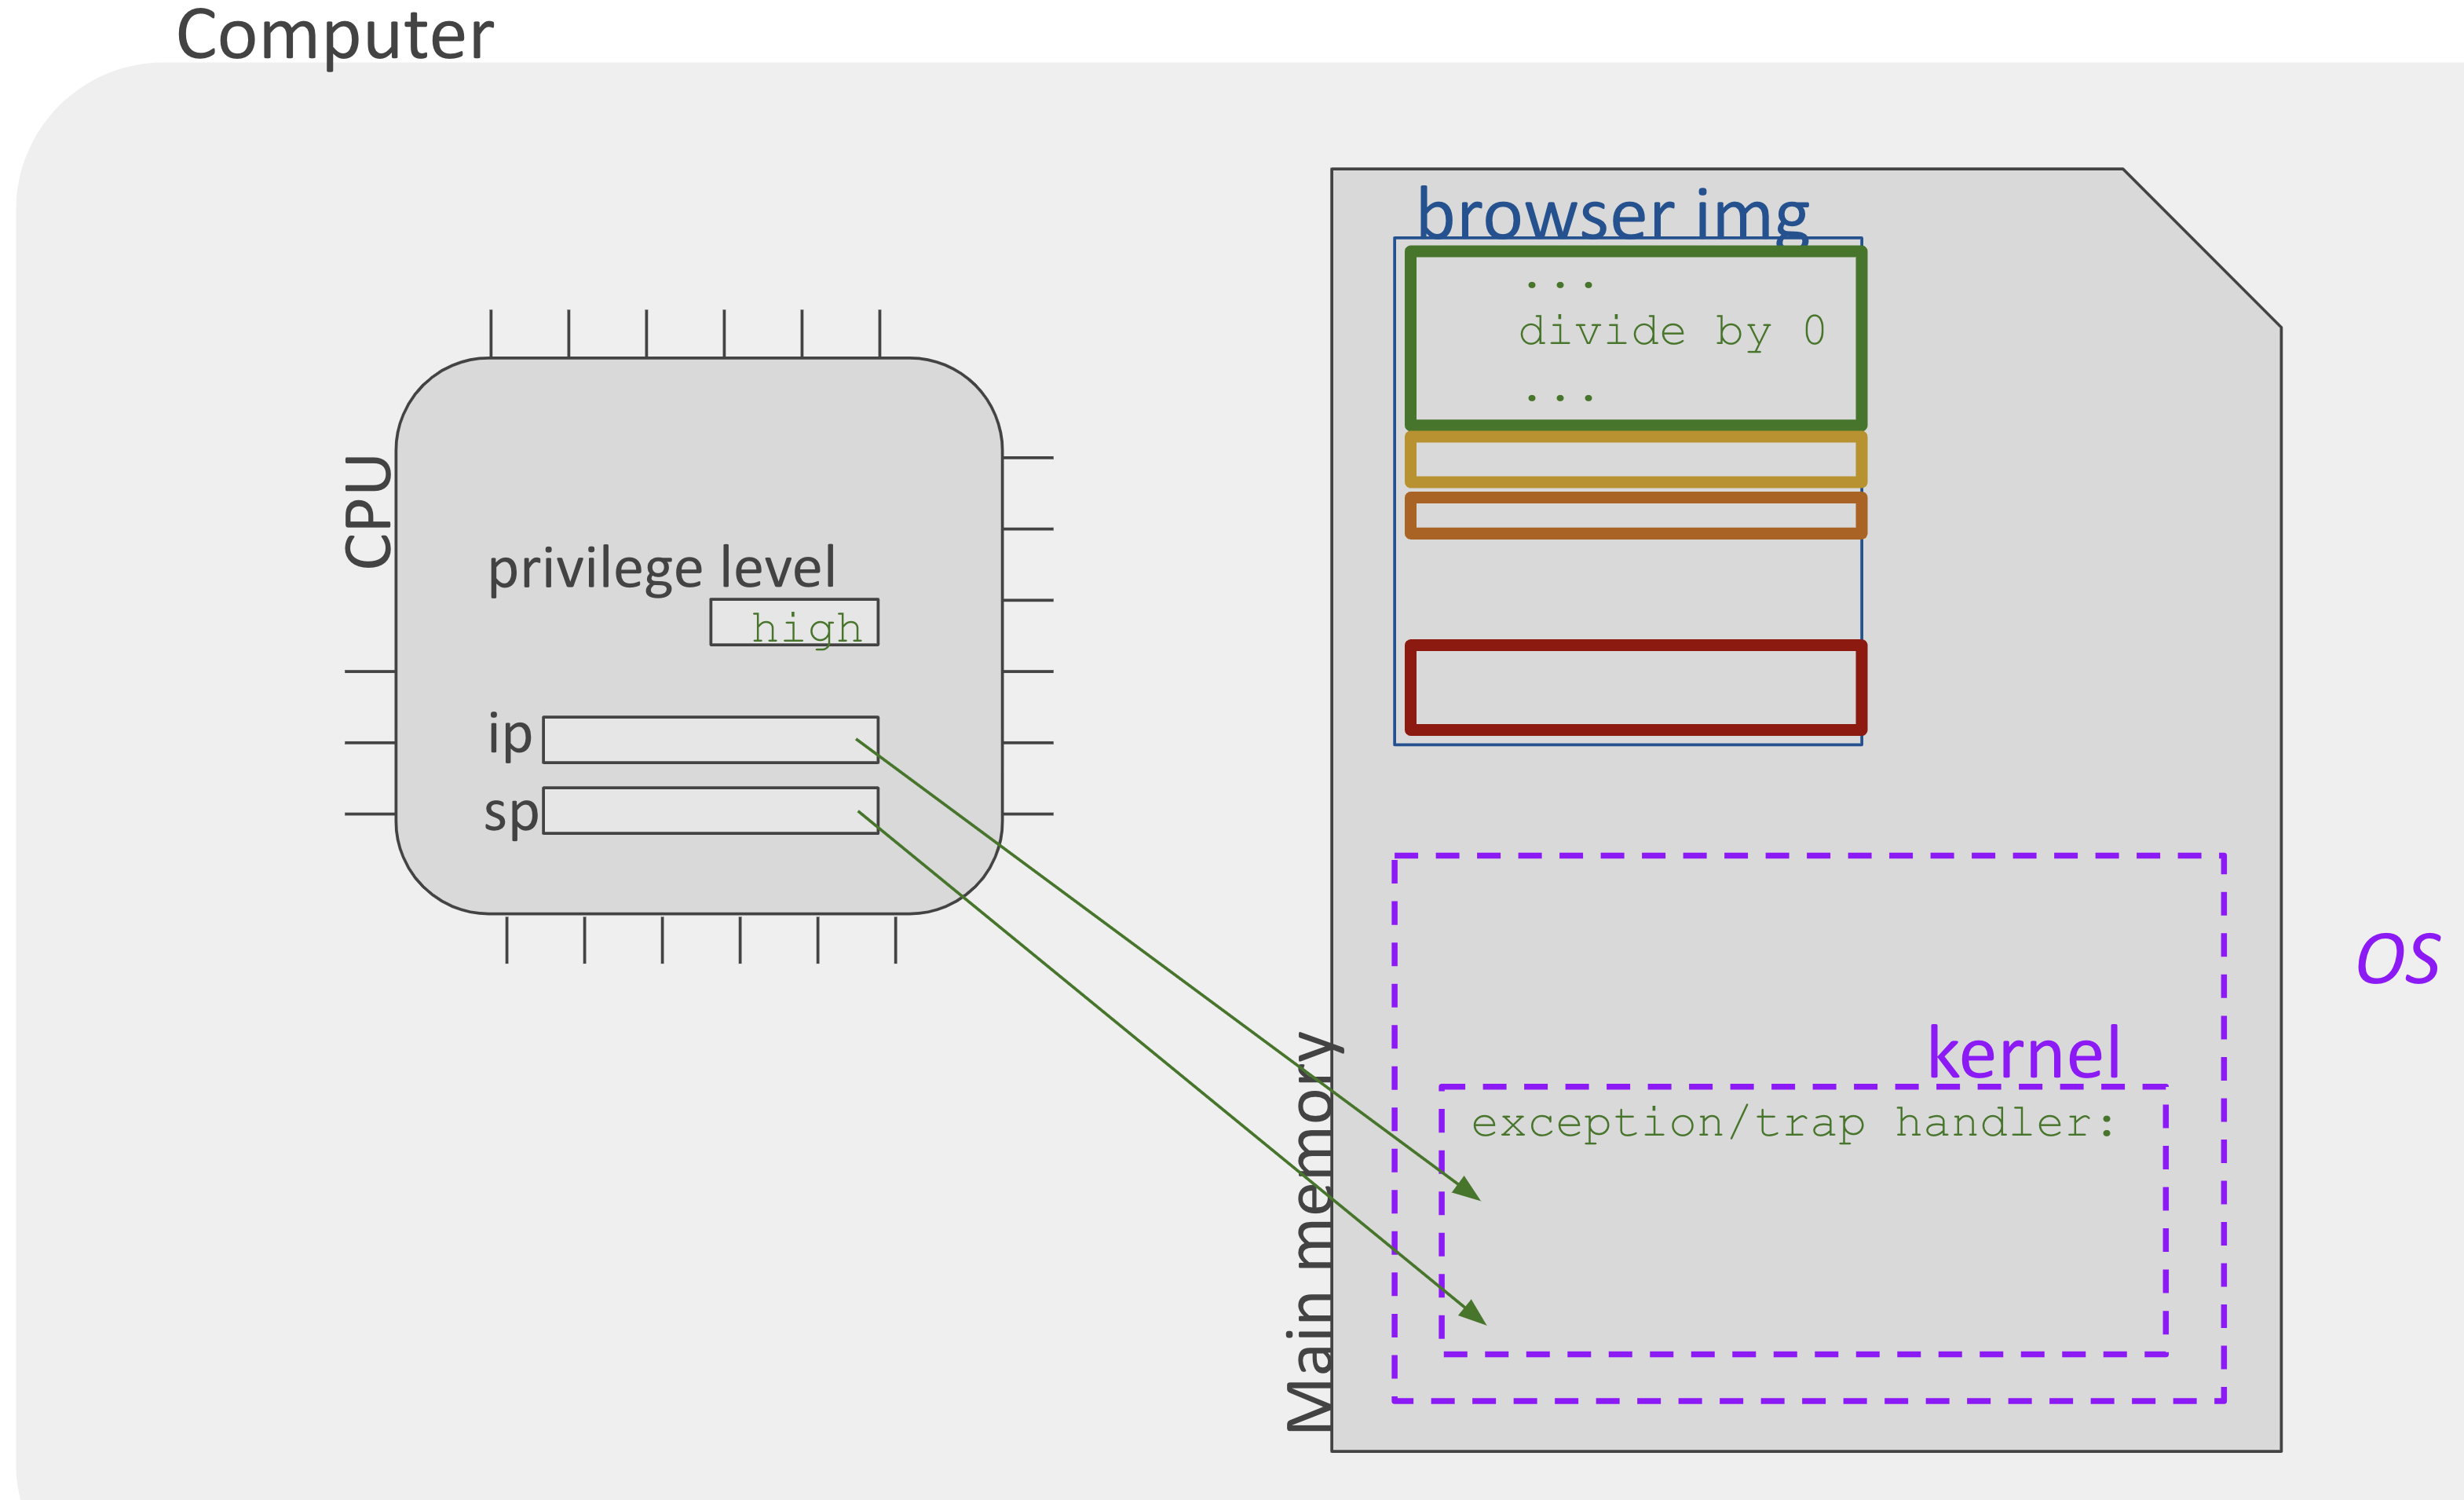
\includegraphics[width=0.95\textwidth]{chapters/L3/images/exception.png}
\end{center}
\end{minipage} 
\hfill 
\vline 
\hfill 
\begin{minipage}[htp]{0.45\textwidth}
\subsubsection*{Interrupt Handling}
Interrupts are triggered by external events and are managed by both hardware and software. The hardware raises the interrupt, and the kernel (via an interrupt handler) processes it.
\vspace{8px}
\begin{center} 
  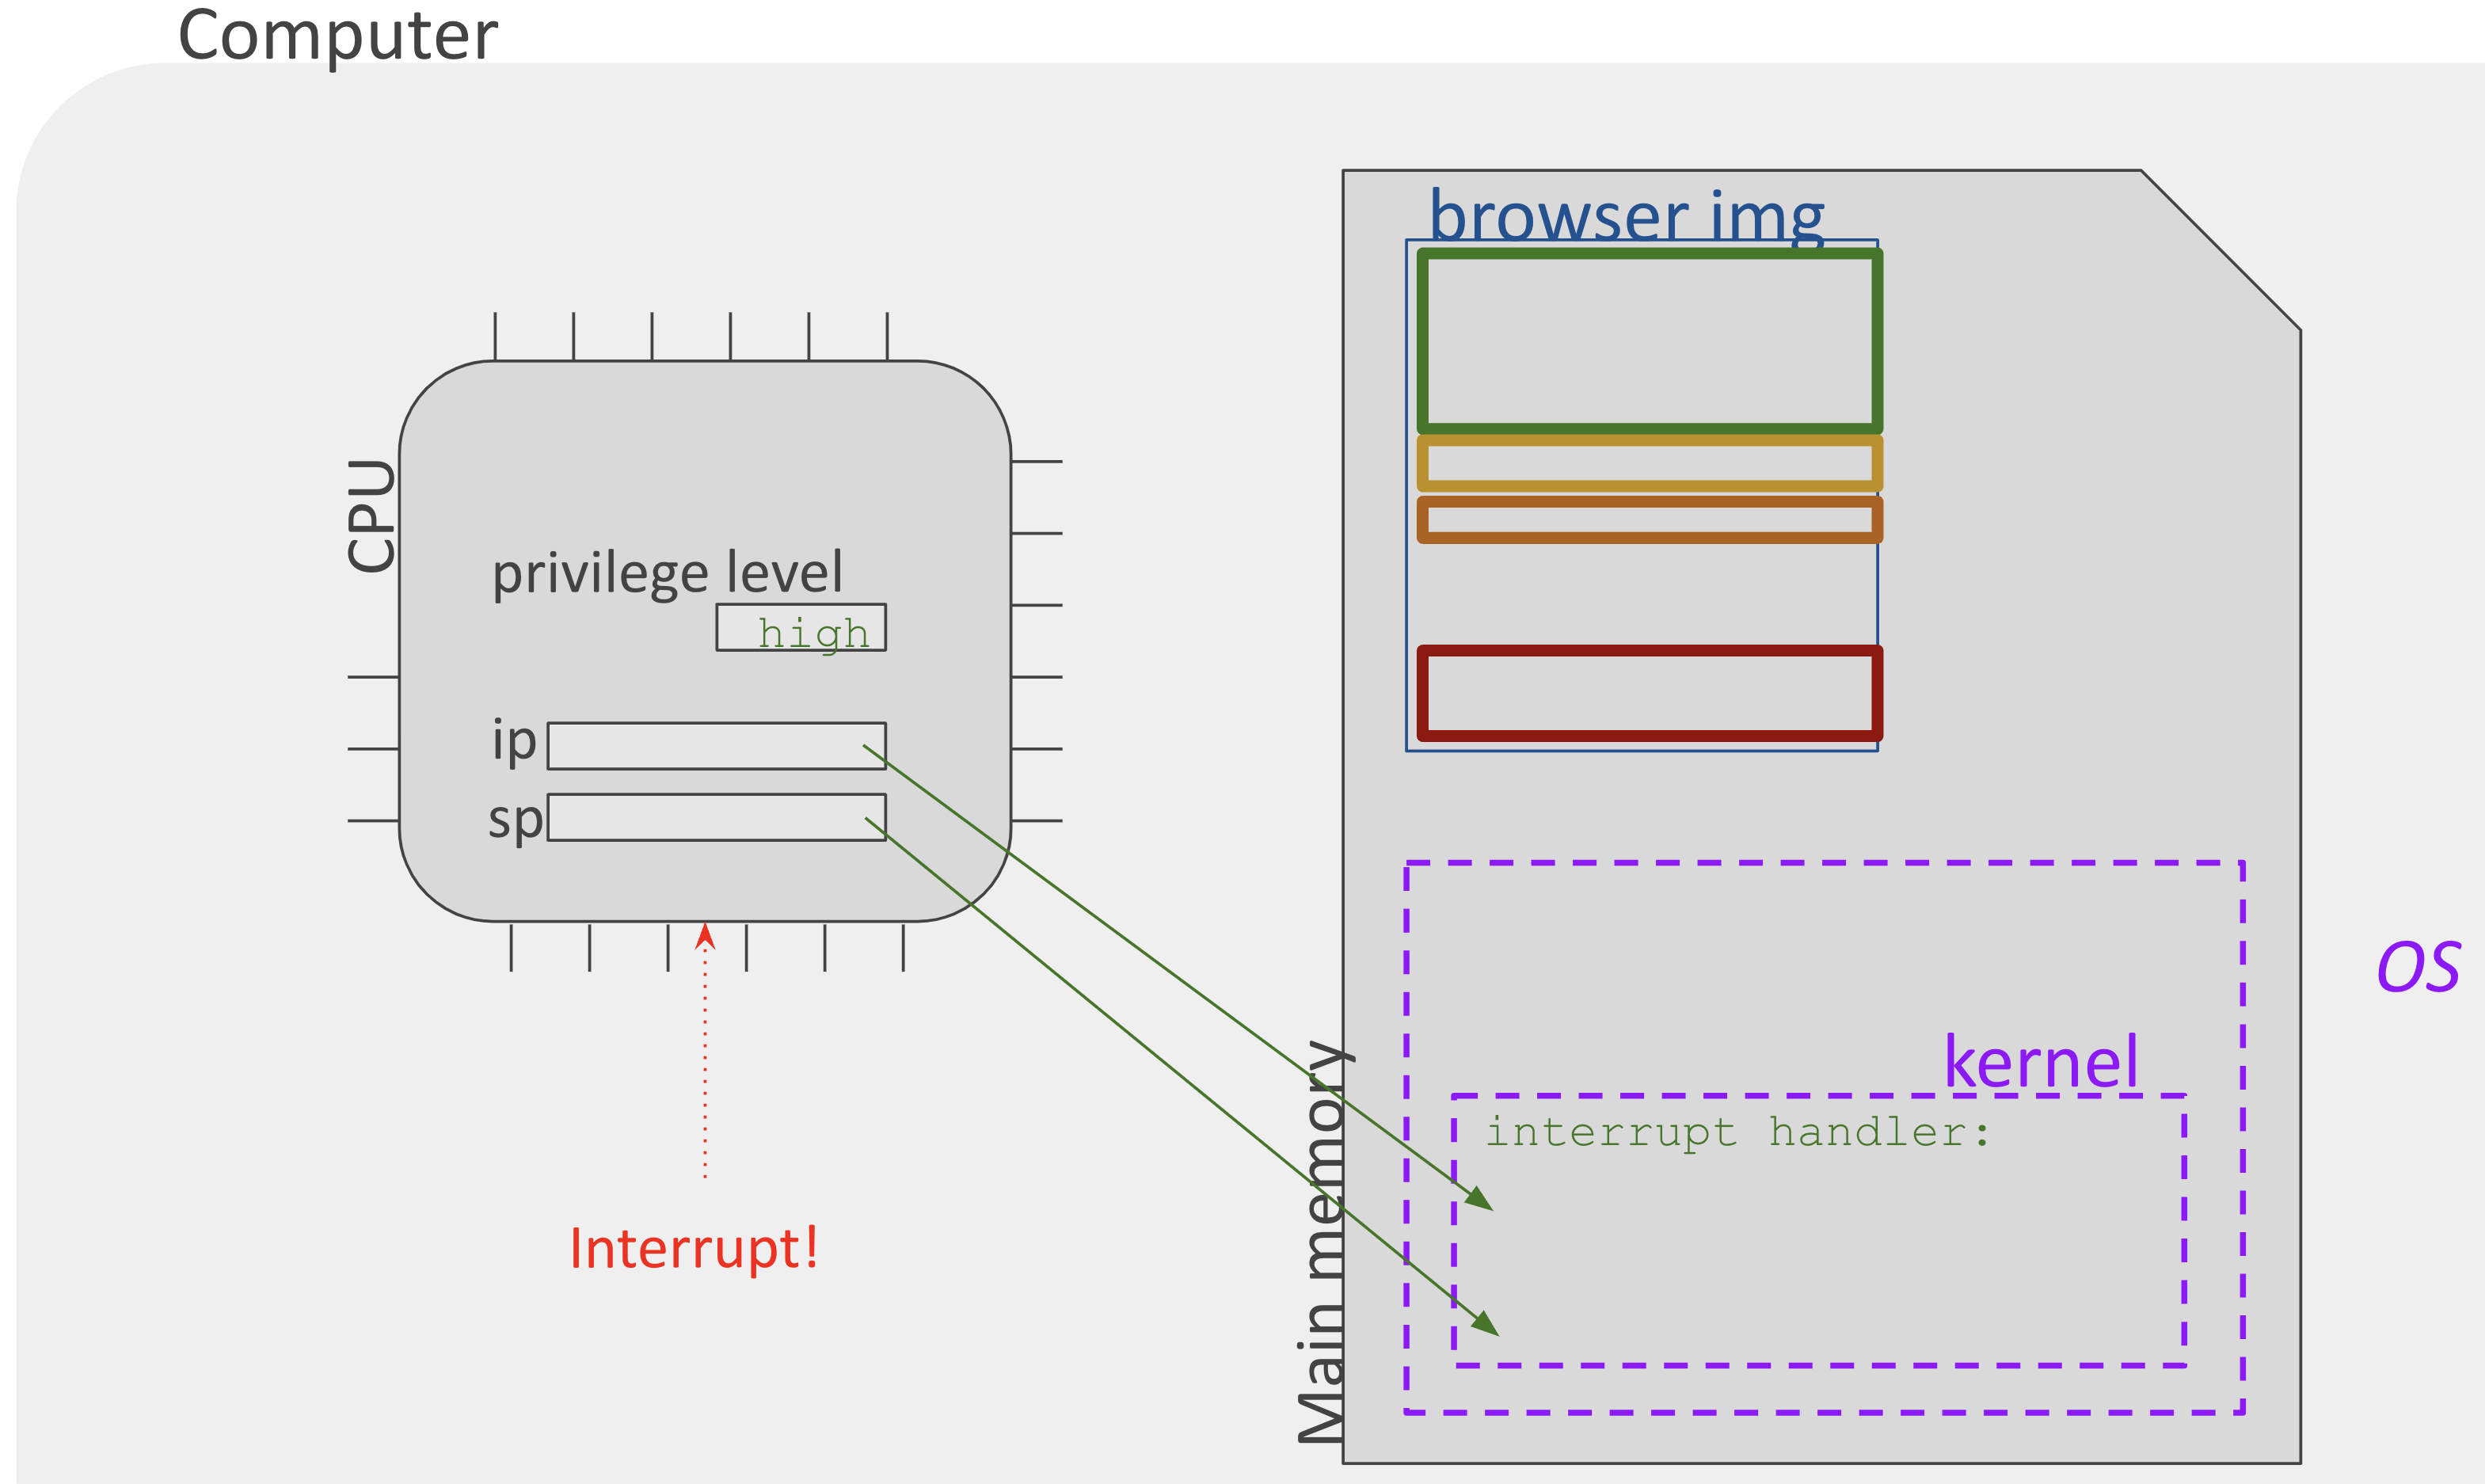
\includegraphics[width=0.95\textwidth]{chapters/L3/images/interrupt.png}
\end{center}
\end{minipage}

\subsubsection{The Timer Interrupt}
\begin{definition}[Timer Interrupt]
The timer interrupt is raised at regular intervals (typically every few milliseconds). Its handler invokes the OS scheduler to decide which process runs next, ensuring that no process monopolizes the CPU.
\end{definition}
\vspace{15px}
\newpage
\subsubsection{The OS Scheduler}
The OS scheduler manages the state transitions of processes (Running, Blocked, Ready) based on various scheduling algorithms, thereby ensuring equitable CPU access.

\begin{center}
  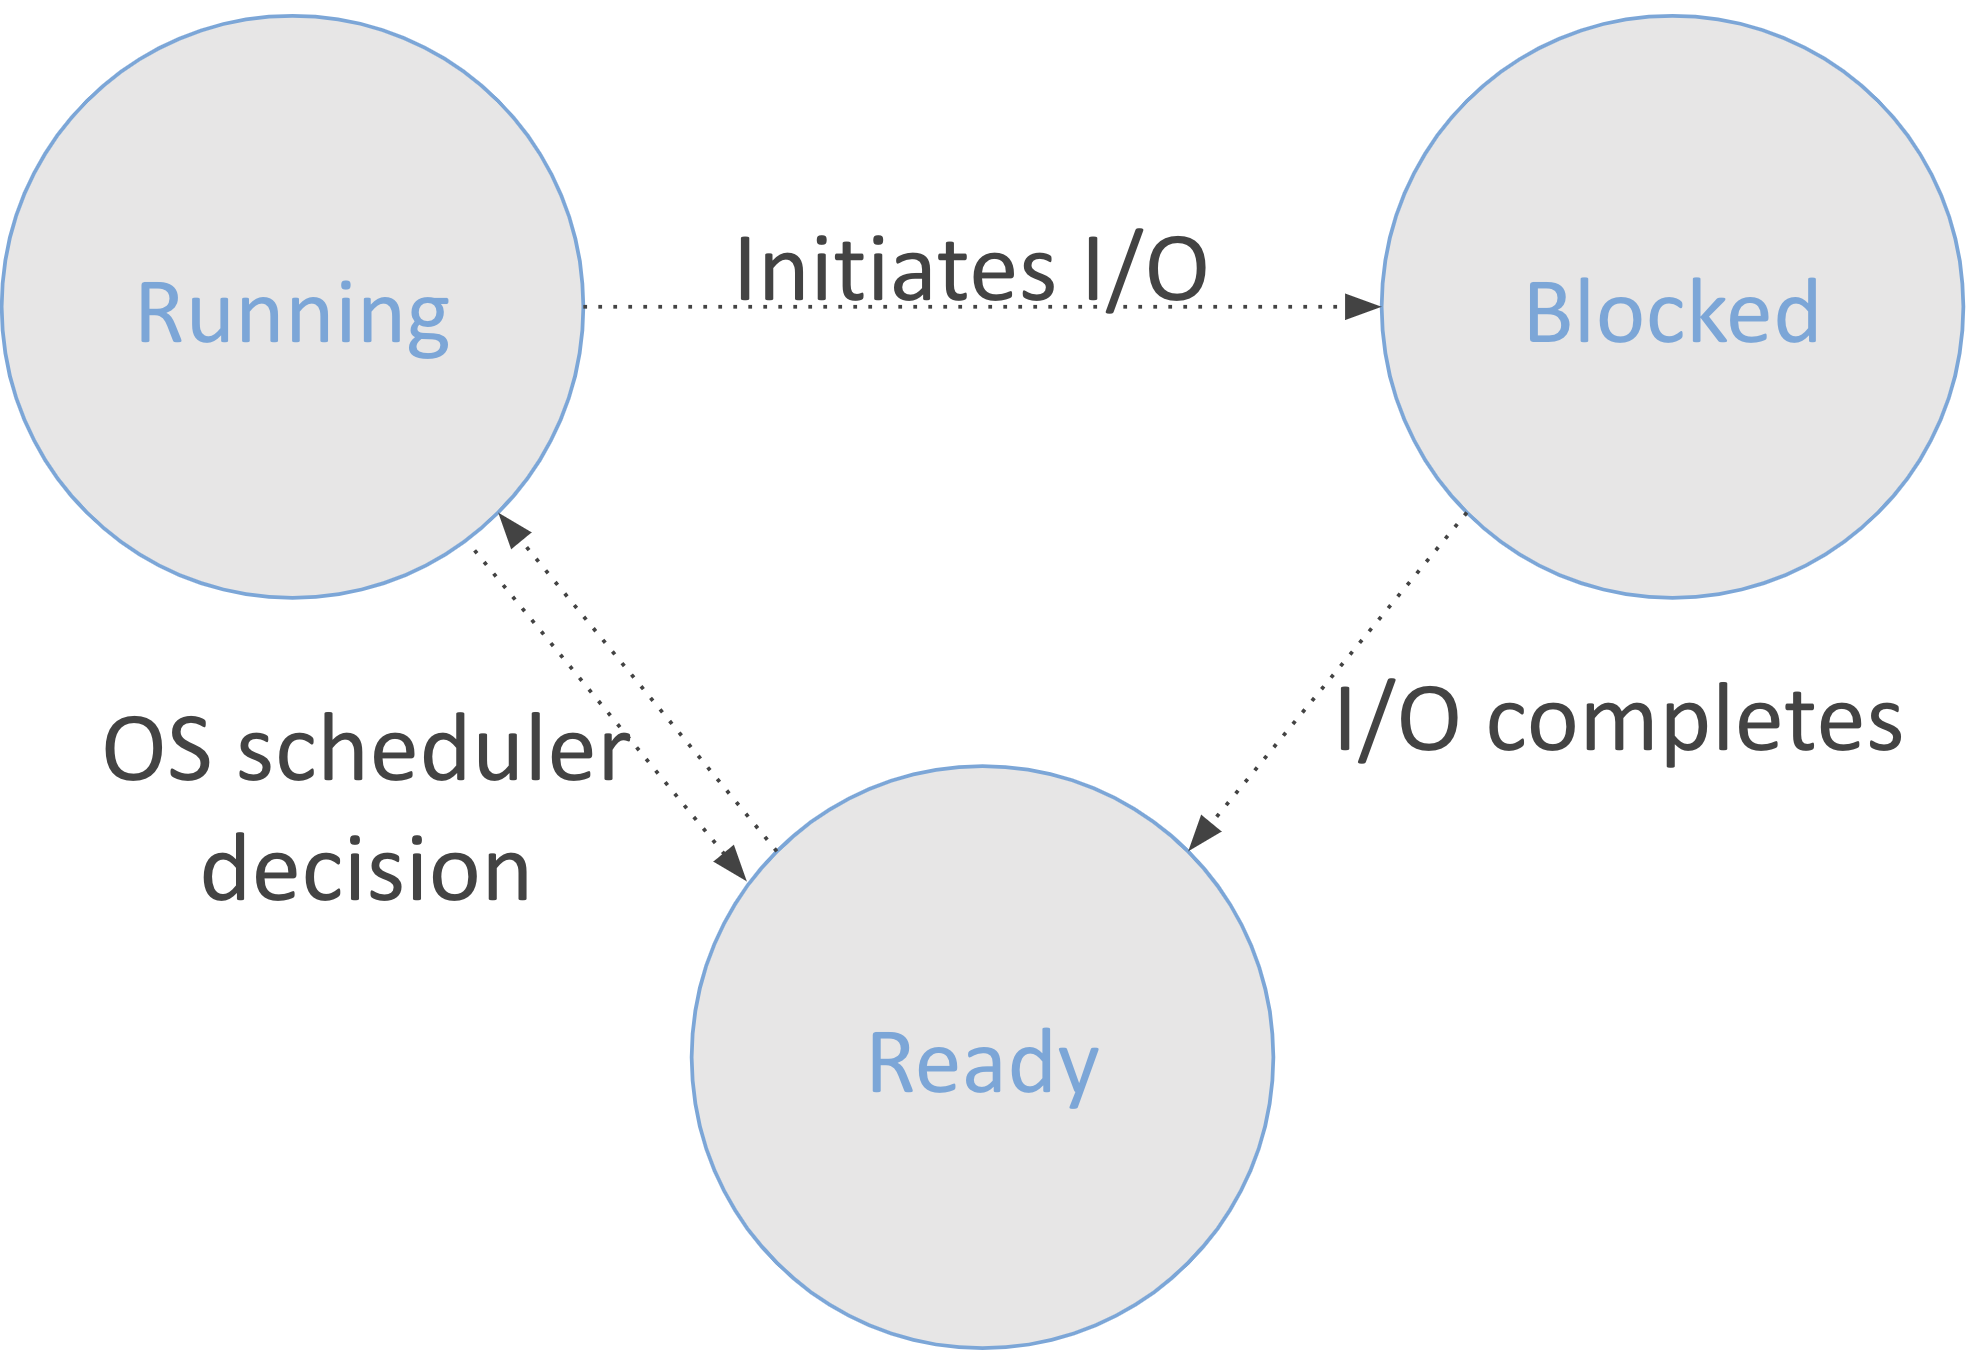
\includegraphics[width=0.45\textwidth]{chapters/L3/images/os-scheduler.png}
\end{center}

\subsection*{Summary - Limited Direct Execution}
\begin{itemize}
  \item[-] Normal threads execute in low privilege.
  \item[-] Operations requiring high privilege are performed via syscalls, exceptions, or interrupts, which invoke the kernel.
  \item[-] Timer interrupts ensure that the OS scheduler periodically gains control, maintaining fairness.
\end{itemize}

Limited direct execution is essential for safely and efficiently sharing the CPU among multiple processes.

\section{Executing Syscalls --- Process Management}

Processes are created, modified, and terminated using various syscalls. We now discuss the key syscalls involved in process management.

\subsection{Syscall Definitions}

\begin{definition}[Exit Syscall]
The \texttt{exit} syscall terminates a process. It never returns because, by the time control would return to the calling process, the process no longer exists.
\end{definition}

\begin{figure}[htp]
  \centering
  \begin{minipage}[htp]{0.45\textwidth}
\begin{cc}
_exit(0);
. 
. 
. 
. 
. 
. 
. 
. 
. 
. 
. 
\end{cc}
  \end{minipage}
  \hfill
  \vline
  \hfill
  \begin{minipage}[htp]{0.45\textwidth}
    \centering
    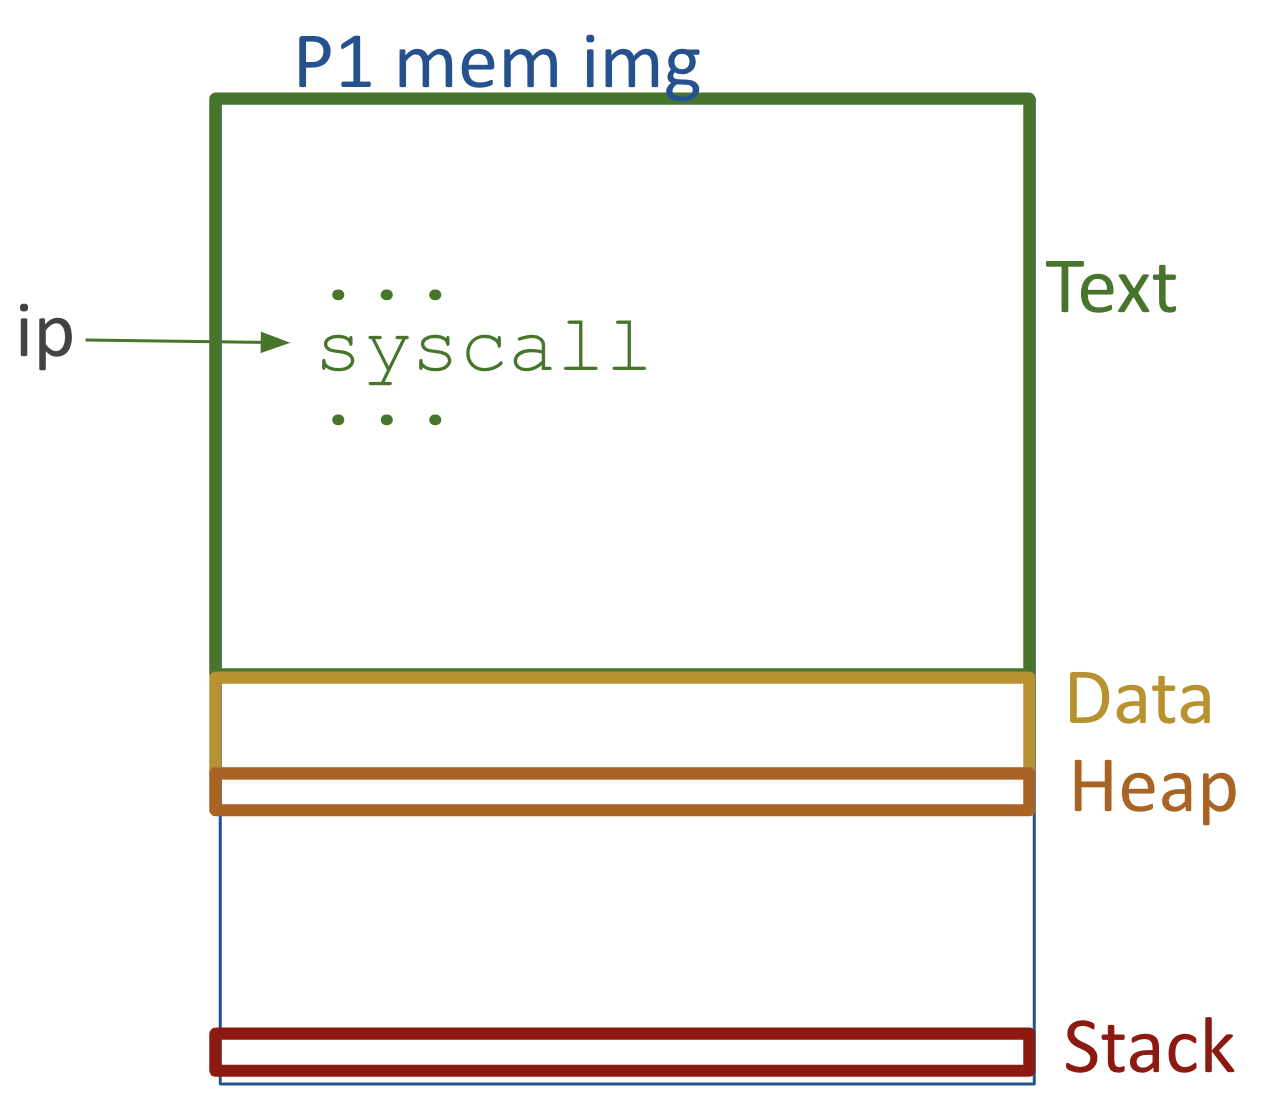
\includegraphics[width=0.8\textwidth]{chapters/L3/images/exit.png}
  \end{minipage}
  \caption{Exit Syscall: Code snippet and stack visualization.}
\end{figure}
\newpage
\begin{definition}[Exec Syscall]
The \texttt{exec} syscall replaces the current process image with a new program. It preserves the process ID and file descriptors while discarding the old program's code, data, and stack. On success, it does not return; on failure, it returns \texttt{-1}.
\end{definition}

\begin{figure}[htp]
  \centering
  \begin{minipage}[b]{0.45\textwidth}
    \begin{cc}
execvp("date", args);











    \end{cc}
  \end{minipage}
  \hfill
  \vline
  \hfill
  \begin{minipage}[b]{0.45\textwidth}
    \centering
    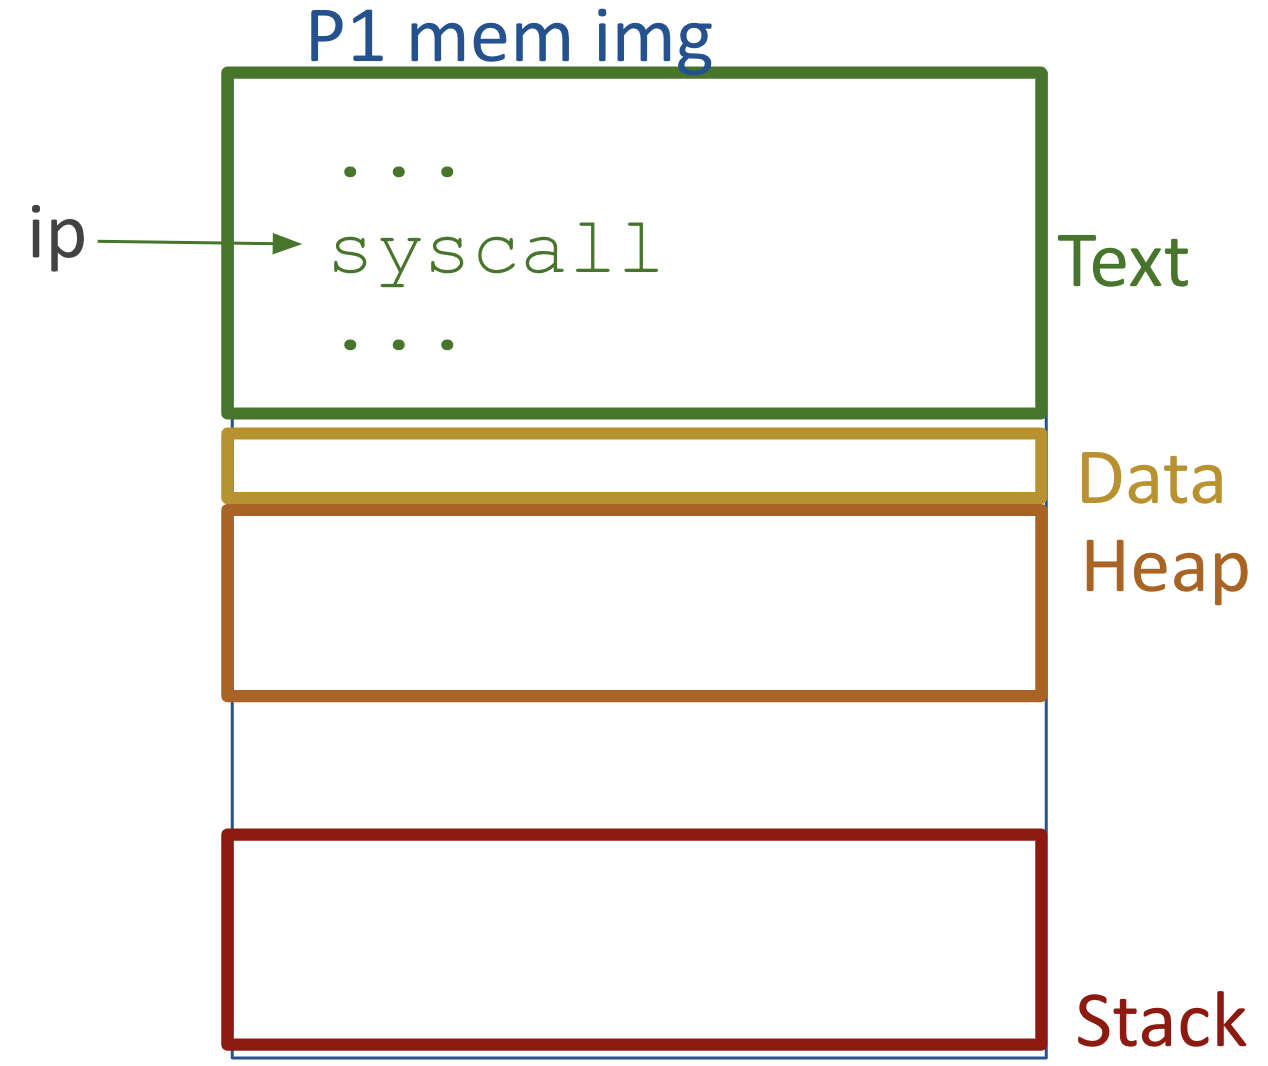
\includegraphics[width=0.8\textwidth]{chapters/L3/images/exec.png}
  \end{minipage}
  \caption{Exec Syscall: Code snippet and process image.}
\end{figure}

\begin{definition}[Fork Syscall]
The \texttt{fork} syscall creates a new child process by duplicating the calling process. Both the parent and child continue execution from the point of the fork, but in separate memory spaces. The fork returns \texttt{0} to the child and the child's process ID (PID) to the parent.
\end{definition}

\begin{figure}[htp]
  \centering
  \begin{minipage}[b]{0.45\textwidth}
    \begin{cc}
int fs = fork();
if (fs == 0) {
   // Child process code
} else {
   // Parent process code
}




    \end{cc}
  \end{minipage}
  \hfill
  \vline
  \hfill
  \begin{minipage}[b]{0.45\textwidth}
    \centering
    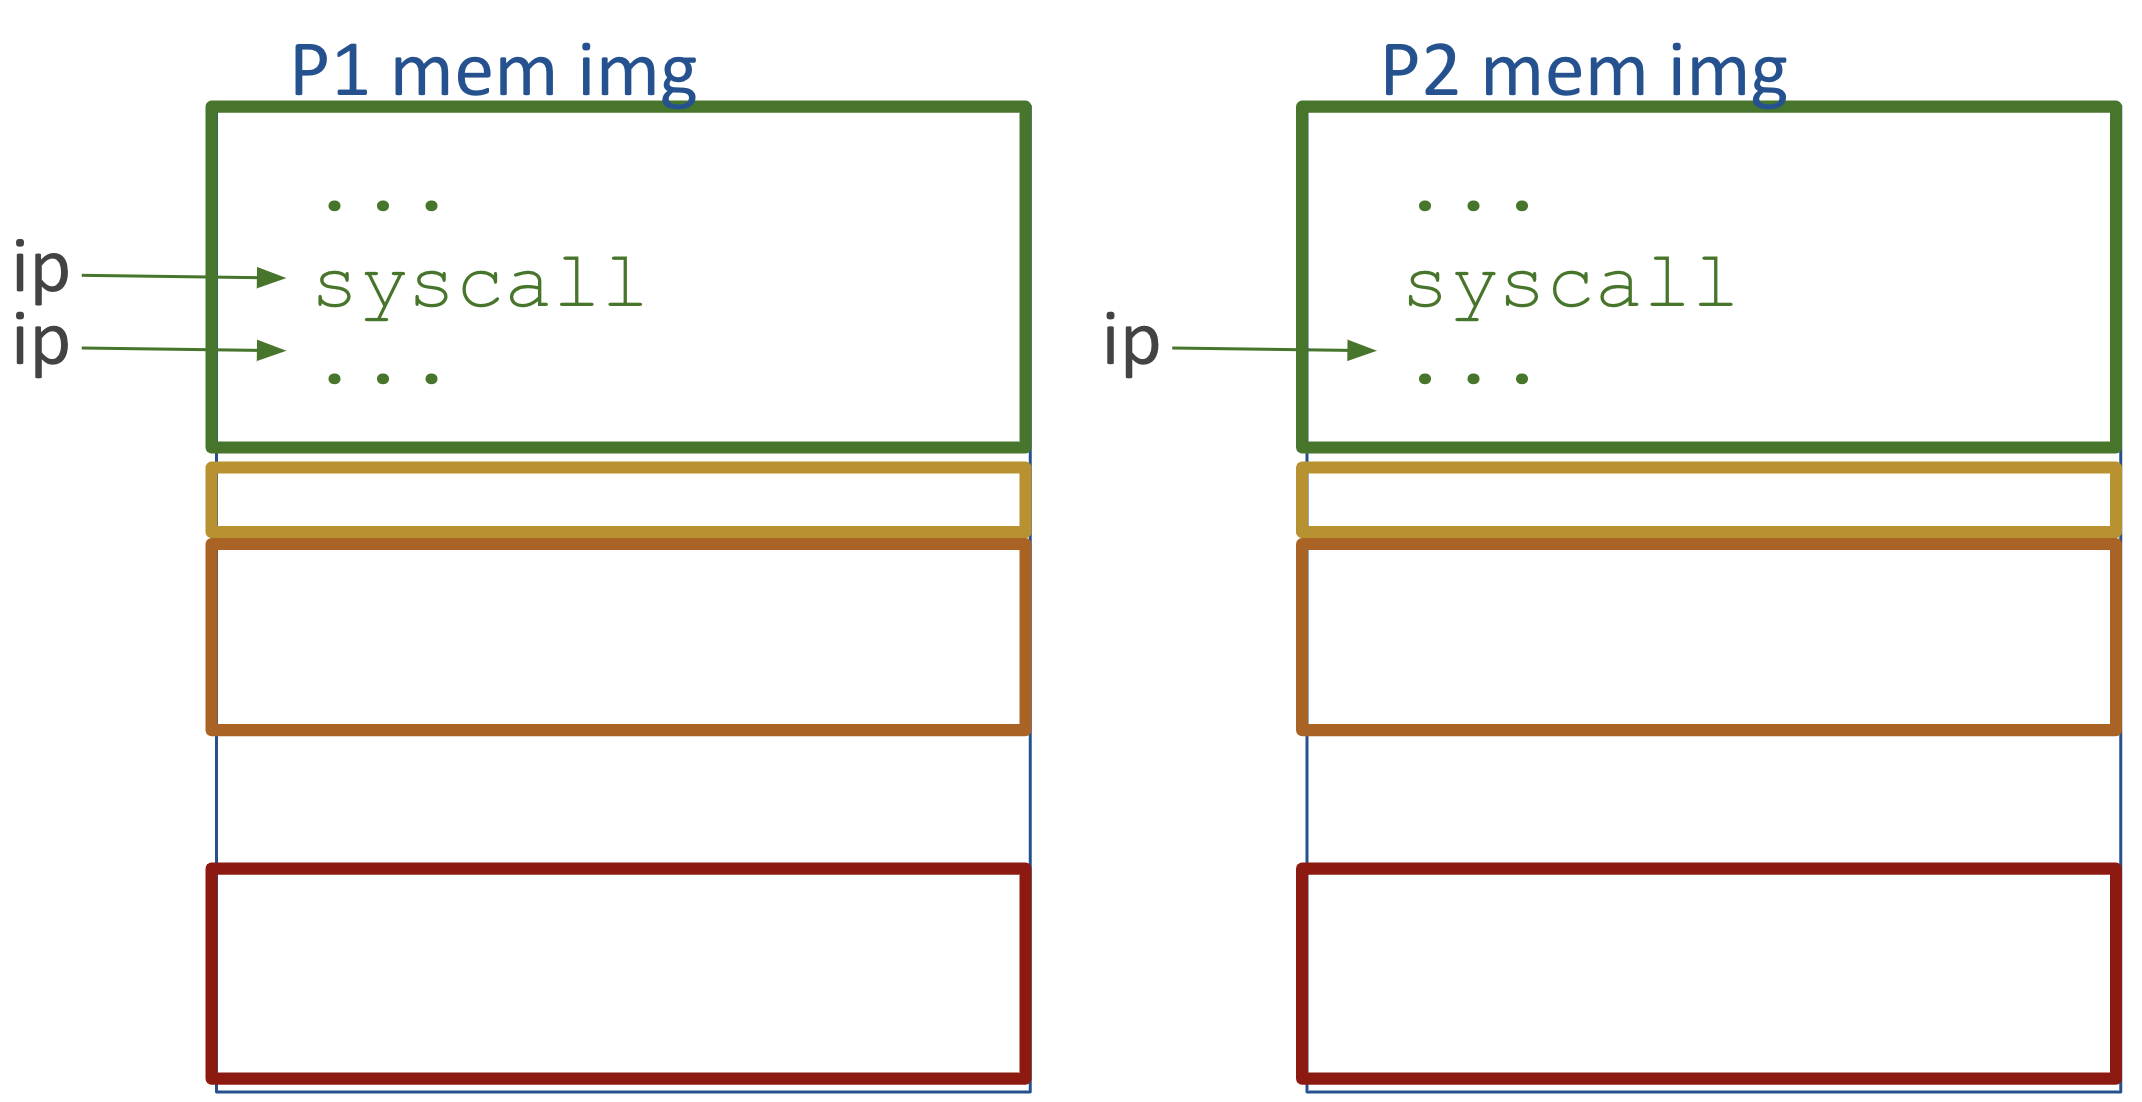
\includegraphics[width=1.25\textwidth]{chapters/L3/images/fork.png}
  \end{minipage}
  \caption{Fork Syscall: Example code and the resulting stack layout.}
\end{figure}

\begin{definition}[Wait Syscall]
The \texttt{wait} syscall allows a parent process to block until one of its child processes terminates. If no child process exists, \texttt{wait()} returns an error.
\end{definition}

\subsection{Process Creation and Cleanup}

Processes are typically created by combining the \texttt{fork} and \texttt{exec} syscalls. For example:
\begin{cc}
int fs = fork();
if (fs == 0) {
   execvp("date", args);
} else {
   wait(fs);
}
\end{cc}

When a parent process calls \texttt{wait()}, it is blocked until a child terminates, ensuring proper cleanup of child processes.
\newpage
\section{The OS Process Graph}
The OS maintains a process graph where each square represents a process and each arrow indicates the parent-child relationship. These kind of graphs are crucial for understanding process creation and hierarchy.

\begin{center}
  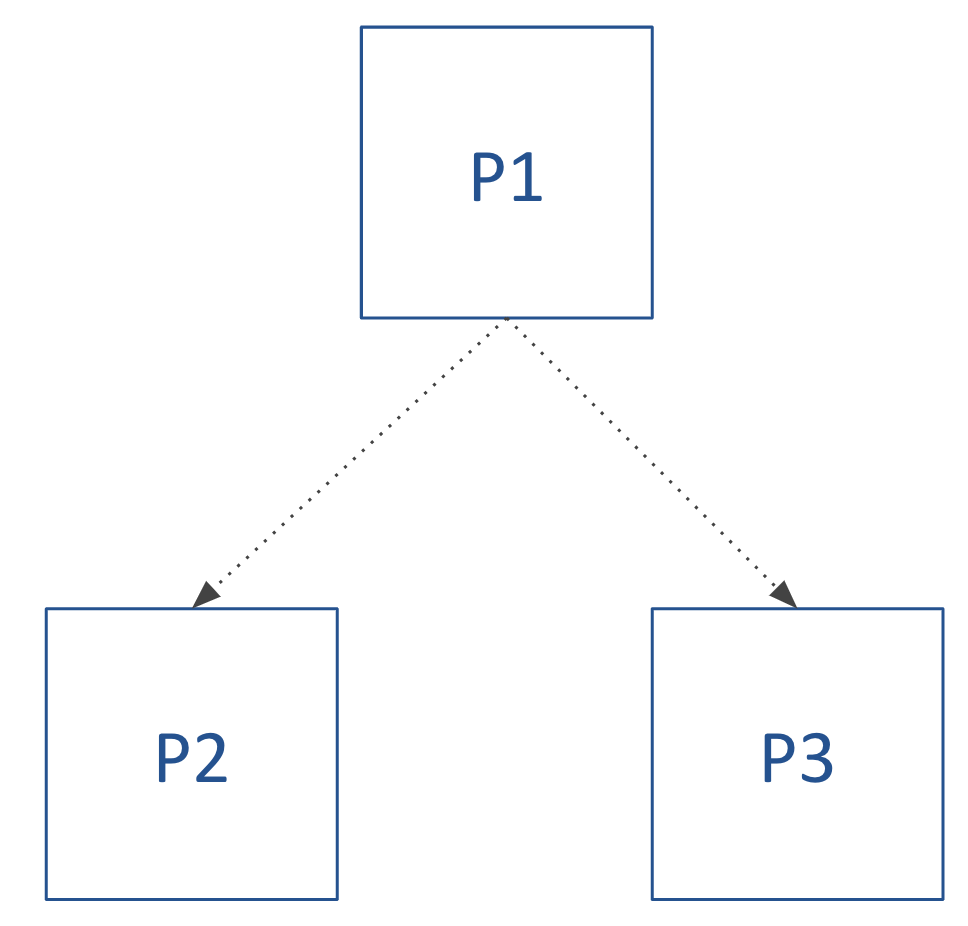
\includegraphics[width=0.25\textwidth]{chapters/L3/images/graph.png}
\end{center}

\section{Key Processes in the OS}

Some critical processes managed by the OS include:
\begin{itemize}
  \item[-] \textbf{GUI Processes:} Manage the graphical user interface.
  \item[-] \textbf{Terminal Processes:} Handle command-line interactions.
  \item[-] \textbf{Init Process:} The first process created by the kernel, responsible for starting system services.
  \item[-] \textbf{Idle Process:} Executes when no other process is runnable.
\end{itemize}

\subsection*{Conclusion - The Role of Syscalls}

Syscalls provide the interface through which processes access system resources such as storage and networks. They also facilitate self-management operations, including process creation, modification, and cleanup. Through mechanisms such as limited direct execution, exceptions, and interrupts, the OS ensures that the CPU is shared safely and efficiently among all processes.
 

\end{document}
